\documentclass[a4paper]{article}

\def\npart {III}
\def\nterm {Michaelmas}
\def\nyear {2016}
\def\nlecturer {O. Randal-Williams}
\def\ncourse {Algebraic Topology}
\def\nlectures {MWF.12}

% Imports
\ifx \nextra \undefined
  \usepackage[pdftex,
    hidelinks,
    pdfauthor={Dexter Chua},
    pdfsubject={Cambridge Maths Notes: Part \npart\ - \ncourse},
    pdftitle={Part \npart\ - \ncourse},
  pdfkeywords={Cambridge Mathematics Maths Math \npart\ \nterm\ \nyear\ \ncourse}]{hyperref}
  \title{Part \npart\ - \ncourse}
\else
  \usepackage[pdftex,
    hidelinks,
    pdfauthor={Dexter Chua},
    pdfsubject={Cambridge Maths Notes: Part \npart\ - \ncourse\ (\nextra)},
    pdftitle={Part \npart\ - \ncourse\ (\nextra)},
  pdfkeywords={Cambridge Mathematics Maths Math \npart\ \nterm\ \nyear\ \ncourse\ \nextra}]{hyperref}

  \title{Part \npart\ - \ncourse \\ {\Large \nextra}}
\fi

\author{Lectured by \nlecturer \\\small Notes taken by Dexter Chua}
\date{\nterm\ \nyear}

\usepackage{alltt}
\usepackage{amsfonts}
\usepackage{amsmath}
\usepackage{amssymb}
\usepackage{amsthm}
\usepackage{booktabs}
\usepackage{caption}
\usepackage{enumitem}
\usepackage{fancyhdr}
\usepackage{graphicx}
\usepackage{mathtools}
\usepackage{microtype}
\usepackage{multirow}
\usepackage{pdflscape}
\usepackage{pgfplots}
\usepackage{siunitx}
\usepackage{tabularx}
\usepackage{tikz}
\usepackage{tkz-euclide}
\usepackage[normalem]{ulem}
\usepackage[all]{xy}

\pgfplotsset{compat=1.12}

\pagestyle{fancyplain}
\lhead{\emph{\nouppercase{\leftmark}}}
\ifx \nextra \undefined
  \rhead{
    \ifnum\thepage=1
    \else
      \npart\ \ncourse
    \fi}
\else
  \rhead{
    \ifnum\thepage=1
    \else
      \npart\ \ncourse\ (\nextra)
    \fi}
\fi
\usetikzlibrary{arrows}
\usetikzlibrary{decorations.markings}
\usetikzlibrary{decorations.pathmorphing}
\usetikzlibrary{positioning}
\usetikzlibrary{fadings}
\usetikzlibrary{intersections}
\usetikzlibrary{cd}

\newcommand*{\Cdot}{\raisebox{-0.25ex}{\scalebox{1.5}{$\cdot$}}}
\newcommand {\pd}[2][ ]{
  \ifx #1 { }
    \frac{\partial}{\partial #2}
  \else
    \frac{\partial^{#1}}{\partial #2^{#1}}
  \fi
}

% Theorems
\theoremstyle{definition}
\newtheorem*{aim}{Aim}
\newtheorem*{axiom}{Axiom}
\newtheorem*{claim}{Claim}
\newtheorem*{cor}{Corollary}
\newtheorem*{defi}{Definition}
\newtheorem*{eg}{Example}
\newtheorem*{fact}{Fact}
\newtheorem*{law}{Law}
\newtheorem*{lemma}{Lemma}
\newtheorem*{notation}{Notation}
\newtheorem*{prop}{Proposition}
\newtheorem*{thm}{Theorem}

\renewcommand{\labelitemi}{--}
\renewcommand{\labelitemii}{$\circ$}
\renewcommand{\labelenumi}{(\roman{*})}

\let\stdsection\section
\renewcommand\section{\newpage\stdsection}

% Strike through
\def\st{\bgroup \ULdepth=-.55ex \ULset}

% Maths symbols
\newcommand{\bra}{\langle}
\newcommand{\ket}{\rangle}

\newcommand{\N}{\mathbb{N}}
\newcommand{\Z}{\mathbb{Z}}
\newcommand{\Q}{\mathbb{Q}}
\renewcommand{\H}{\mathbb{H}}
\newcommand{\R}{\mathbb{R}}
\newcommand{\C}{\mathbb{C}}
\newcommand{\Prob}{\mathbb{P}}
\renewcommand{\P}{\mathbb{P}}
\newcommand{\E}{\mathbb{E}}
\newcommand{\F}{\mathbb{F}}
\newcommand{\cU}{\mathcal{U}}
\newcommand{\RP}{\mathbb{RP}}
\newcommand{\CP}{\mathbb{CP}}

\newcommand{\ph}{\,\cdot\,}

\DeclareMathOperator{\sech}{sech}
\DeclareMathOperator{\cosech}{cosech}
\DeclareMathOperator{\cosec}{cosec}

\DeclareMathOperator{\covol}{covol}
\DeclareMathOperator{\vol}{vol}

\let\Im\relax
\let\Re\relax
\DeclareMathOperator{\Im}{Im}
\DeclareMathOperator{\Re}{Re}
\DeclareMathOperator{\im}{im}
\DeclareMathOperator{\image}{image}
\DeclareMathOperator{\Ann}{Ann}

\DeclareMathOperator*{\res}{res}
\DeclareMathOperator{\Res}{Res}
\DeclareMathOperator{\Ind}{Ind}

\DeclareMathOperator{\tr}{tr}
\DeclareMathOperator{\diag}{diag}
\DeclareMathOperator{\rank}{rank}
\DeclareMathOperator{\card}{card}
\DeclareMathOperator{\spn}{span}
\DeclareMathOperator{\adj}{adj}

\DeclareMathOperator{\erf}{erf}
\DeclareMathOperator{\erfc}{erfc}

\DeclareMathOperator{\ord}{ord}
\DeclareMathOperator{\Sym}{Sym}

\DeclareMathOperator{\sgn}{sgn}
\DeclareMathOperator{\orb}{orb}
\DeclareMathOperator{\stab}{stab}
\DeclareMathOperator{\ccl}{ccl}

\DeclareMathOperator{\lcm}{lcm}
\DeclareMathOperator{\hcf}{hcf}

\DeclareMathOperator{\Int}{Int}
\DeclareMathOperator{\id}{id}

\DeclareMathOperator{\betaD}{beta}
\DeclareMathOperator{\gammaD}{gamma}
\DeclareMathOperator{\Poisson}{Poisson}
\DeclareMathOperator{\binomial}{binomial}
\DeclareMathOperator{\multinomial}{multinomial}
\DeclareMathOperator{\Bernoulli}{Bernoulli}
\DeclareMathOperator{\like}{like}

\DeclareMathOperator{\var}{var}
\DeclareMathOperator{\cov}{cov}
\DeclareMathOperator{\bias}{bias}
\DeclareMathOperator{\mse}{mse}
\DeclareMathOperator{\corr}{corr}

\DeclareMathOperator{\otp}{otp}
\DeclareMathOperator{\dom}{dom}

\DeclareMathOperator{\Root}{Root}
\DeclareMathOperator{\supp}{supp}
\DeclareMathOperator{\rel}{rel}
\DeclareMathOperator{\Hom}{Hom}
\DeclareMathOperator{\Aut}{Aut}
\DeclareMathOperator{\Gal}{Gal}
\DeclareMathOperator{\Mat}{Mat}
\DeclareMathOperator{\End}{End}
\DeclareMathOperator{\Char}{char}
\DeclareMathOperator{\ev}{ev}
\DeclareMathOperator{\St}{St}
\DeclareMathOperator{\Lk}{Lk}
\DeclareMathOperator{\disc}{disc}
\DeclareMathOperator{\Isom}{Isom}
\DeclareMathOperator{\length}{length}
\DeclareMathOperator{\energy}{energy}
\DeclareMathOperator{\area}{area}
\DeclareMathOperator{\Syl}{Syl}
\DeclareMathOperator{\cl}{cl}
\DeclareMathOperator{\fix}{fix}

\newcommand{\GL}{\mathrm{GL}}
\newcommand{\SL}{\mathrm{SL}}
\newcommand{\PGL}{\mathrm{PGL}}
\newcommand{\PSL}{\mathrm{PSL}}
\newcommand{\PSU}{\mathrm{PSU}}
\newcommand{\Or}{\mathrm{O}}
\newcommand{\SO}{\mathrm{SO}}
\newcommand{\U}{\mathrm{U}}
\newcommand{\SU}{\mathrm{SU}}

\renewcommand{\d}{\mathrm{d}}
\newcommand{\D}{\mathrm{D}}

\tikzset{->/.style = {decoration={markings,
                                  mark=at position 1 with {\arrow[scale=2]{latex'}}},
                      postaction={decorate}}}
\tikzset{<-/.style = {decoration={markings,
                                  mark=at position 0 with {\arrowreversed[scale=2]{latex'}}},
                      postaction={decorate}}}
\tikzset{<->/.style = {decoration={markings,
                                   mark=at position 0 with {\arrowreversed[scale=2]{latex'}},
                                   mark=at position 1 with {\arrow[scale=2]{latex'}}},
                       postaction={decorate}}}
\tikzset{->-/.style = {decoration={markings,
                                   mark=at position #1 with {\arrow[scale=2]{latex'}}},
                       postaction={decorate}}}
\tikzset{-<-/.style = {decoration={markings,
                                   mark=at position #1 with {\arrowreversed[scale=2]{latex'}}},
                       postaction={decorate}}}

\tikzset{circ/.style = {fill, circle, inner sep = 0, minimum size = 3}}
\tikzset{mstate/.style={circle, draw, blue, text=black, minimum width=0.7cm}}

\definecolor{mblue}{rgb}{0.2, 0.3, 0.8}
\definecolor{morange}{rgb}{1, 0.5, 0}
\definecolor{mgreen}{rgb}{0.1, 0.4, 0.2}
\definecolor{mred}{rgb}{0.5, 0, 0}

\def\drawcirculararc(#1,#2)(#3,#4)(#5,#6){%
    \pgfmathsetmacro\cA{(#1*#1+#2*#2-#3*#3-#4*#4)/2}%
    \pgfmathsetmacro\cB{(#1*#1+#2*#2-#5*#5-#6*#6)/2}%
    \pgfmathsetmacro\cy{(\cB*(#1-#3)-\cA*(#1-#5))/%
                        ((#2-#6)*(#1-#3)-(#2-#4)*(#1-#5))}%
    \pgfmathsetmacro\cx{(\cA-\cy*(#2-#4))/(#1-#3)}%
    \pgfmathsetmacro\cr{sqrt((#1-\cx)*(#1-\cx)+(#2-\cy)*(#2-\cy))}%
    \pgfmathsetmacro\cA{atan2(#2-\cy,#1-\cx)}%
    \pgfmathsetmacro\cB{atan2(#6-\cy,#5-\cx)}%
    \pgfmathparse{\cB<\cA}%
    \ifnum\pgfmathresult=1
        \pgfmathsetmacro\cB{\cB+360}%
    \fi
    \draw (#1,#2) arc (\cA:\cB:\cr);%
}
\newcommand\getCoord[3]{\newdimen{#1}\newdimen{#2}\pgfextractx{#1}{\pgfpointanchor{#3}{center}}\pgfextracty{#2}{\pgfpointanchor{#3}{center}}}

\def\Xint#1{\mathchoice
   {\XXint\displaystyle\textstyle{#1}}%
   {\XXint\textstyle\scriptstyle{#1}}%
   {\XXint\scriptstyle\scriptscriptstyle{#1}}%
   {\XXint\scriptscriptstyle\scriptscriptstyle{#1}}%
   \!\int}
\def\XXint#1#2#3{{\setbox0=\hbox{$#1{#2#3}{\int}$}
     \vcenter{\hbox{$#2#3$}}\kern-.5\wd0}}
\def\ddashint{\Xint=}
\def\dashint{\Xint-}


\begin{document}
\maketitle
{\small
\setlength{\parindent}{0em}
\setlength{\parskip}{1em}

Algebraic Topology assigns algebraic invariants to topological spaces; it permeates modern pure mathematics. This course will focus on (co)homology, with an emphasis on applications to the topology of manifolds. We will cover singular homology and cohomology, vector bundles and the Thom Isomorphism theorem, and the cohomology of manifolds up to Poincar\'e duality. Time permitting, there will also be some discussion of characteristic classes and cobordism, and conceivably some homotopy theory.

\subsubsection*{Pre-requisites}

Basic topology: topological spaces, compactness and connectedness, at the level of Sutherland's book. The course will not assume any knowledge of Algebraic Topology, but will go quite fast in order to reach more interesting material, so some previous exposure to simplicial homology or the fundamental group would be helpful. The Part III Differential Geometry course will also contain useful, relevant material.

Hatcher's book is especially recommended for the course, but there are many other suitable texts.
}
\tableofcontents

\section{Homotopy}
In this course, ``map'' means ``continuous function''.

\begin{defi}[Homotopy]\index{homotopy}
  Let $X, Y$ be a topological space. A \emph{homotopy} between $f_0, f_1: X \to Y$ is a map $F: [0, 1] \times X \to Y$ such that $F(0, x) = f_0(x)$ and $F(1, x) = f_1(x)$. If such an $F$ exists, we say $f_0$ is \emph{homotopic} to $f_1$, and write $f_0 \simeq f_1$.

  This $\simeq$ defines an equivalence relation on the set of maps from $X$ to $Y$.
\end{defi}
This should be thought of as a continuous deformation from $f_0$ to $f_1$. Note that two homotopic functions can be homotopic in several ways.

If we view homotopic functions as ``the same'', then we have to change our respective notion of isomorphism. To do so, we just write down the usual definition of bijection, but with equality replaced with homotopy.

\begin{defi}[Homotopy equivalence]\index{homotopy equivalence}
  A map $f: X \to Y$ is a \emph{homotopy equivalence} if there is some $g: Y \to X$ such that $f \circ g \simeq \id_X$ and $g \circ f \simeq \id_Y$. We call $g$ the \emph{homotopy inverse}\index{homotopy inverse} to $f$.
\end{defi}

\begin{eg}[Stupid example]
  If $f: X \to Y$ is a homeomorphism, then it is a homotopy equivalence --- we take the actual inverse for the homotopy inverse, since equal functions are homotopic.
\end{eg}

\begin{eg}[Interesting example]
  Let $i: \{0\} \to \R^n$ be the inclusion map. To show this is a homotopy equivalence, we have to find a homotopy inverse. Fortunately, there is only one map $\R^n \to \{0\}$, namely the constant function $0$. We call this $r: \R^n \to \{0\}$. The composition $r \circ i: \{0\} \to \{0\}$ is exactly the identity. So this is good.

  In the other direction, the map $r \circ i: \R^n \to \R^n$ sends everything to $0$. We need to produce a homotopy to the identity. We let $F: [0, 1] \to \R^n \to \R^n$ be
  \[
    F(t, \mathbf{v}) = t\mathbf{v}.
  \]
  We have $F(0, \mathbf{v}) = 0$ and $F(1, \mathbf{v}) = \mathbf{v}$. So this is indeed a homotopy from $r \circ i$ to $\id_{\R^n}$.
\end{eg}

So from the point of view of homotopy, the one-point space $\{0\}$ is the same as $\R^n$. So dimension, or even cardinality, is now a meaningless concept. So what is left?

\begin{eg}[Also interesting example]
  Let $S^n \subseteq \R^{n + 1}$ be the unit sphere, and $i: S^n \hookrightarrow \R^{n + 1} \setminus \{0\}$. We show that this is a homotopy equivalence. We define $r: \R^{n + 1} \setminus \{0\} \to S^n$ by
  \[
    r(\mathbf{v}) = \frac{\mathbf{v}}{\|\mathbf{v}\|}.
  \]
  Again, we have $r \circ i = \id_{S^n}$. In the other direction, we need to construct a path from each $\mathbf{v}$ to $\frac{\mathbf{v}}{\|\mathbf{v}\|}$ in a continuous way. We could do so by
  \begin{align*}
    H: [0, 1] \times (\R^{n + 1} \setminus \{0\}) &\to \R^{n + 1} \setminus \{0\}\\
    (t, \mathbf{v}) &\mapsto (1 - t) \mathbf{v} + t \frac{\mathbf{v}}{\|\mathbf{v}\|}.
  \end{align*}
  We can easily check that this is a homotopy from $\id_{\R^{n + 1}\setminus \{0\}}$ to $i \circ r$.
\end{eg}

While dimension is not a meaningful concept in the homotopy world, we can still say something useful about dimensions using homotopies. Suppose we are given that $\R^n \cong \R^m$. Then we know that $\R^n \setminus \{0\} \cong \R^m \{0\}$. Since these are homotopy equivalent to $S^{n - 1}$ and $S^{m - 1}$, this implies that $S^{n - 1} \sim S^{m - 1}$ are homotopy equivalent. We will later show (by calculating homology of both spheres) that this can only happen if $m \not= n$. So by doing some homotopies, we show that dimension is a meaningful concept if we talk about homeomorphism.

We now see a problem in homotopy theory. If we want to show that two spaces are homotopy equivalent, then we just produce a pair of homotopy inverses. The idea is to assign algebraic objects to each topological space that is homotopy invariant. Thus if two spaces are assigned different algebraic objects, then they cannot be homotopy equivalent.

\section{Chain complex}
The first bit of algebra we need is the notion of a chain complex.
\begin{defi}[Chain complex]\index{chain complex}
  A \emph{chain complex} is a sequence of abelian groups and homomorphisms
  \[
    \begin{tikzcd}
      \cdots \ar[r] & C_3 \ar[r, "d_3"] & C_2 \ar[r, "d_2"] & C_1 \ar[r, "d_1"] & C_0 \ar[r, "d_0"] & 0
    \end{tikzcd}
  \]
  such that
  \[
    d_i \circ d_{i + 1} = 0
  \]
  for all $i$.
\end{defi}

Very related to the notion of a chain complex is a \emph{co}chain complex, which is the same thing with the maps the other way.

\begin{defi}[Cochain complex]\index{cochain complex}
  A \emph{cochain complex} is a sequence of abelian groups and homomorphisms
  \[
    \begin{tikzcd}
      0 \ar[r] & C^0 \ar[r, "d^0"] & C^1 \ar[r, "d^1"] & C^2 \ar[r, "d^2"] & C^3 \ar[r] & \cdots
    \end{tikzcd}
  \]
  such that
  \[
    d^{i + 1} \circ d^i = 0
  \]
  for all $i$.
\end{defi}

\begin{defi}[Differentials]\index{differentials}
  The maps $d^i$ and $d_i$ are known as \emph{differentials}.
\end{defi}
Eventually, we will get lazy and just write all the differentials as $d$.

Given a chain complex, the only thing we know is that the composition of any two maps is zero. In other words, we have $\im d_i \subseteq \ker d_{i + 1}$. We can then ask how good this containment is. Is it that $\im d_i = \ker d_{i + 1}$, or perhaps that $\ker d_{i + 1}$ is huge but $\im d_i$ is trivial? The homology or cohomology measures what happens.

\begin{defi}[Homology]\index{homology}
  The \emph{homology} of a chain complex $C_{\Cdot}$ is
  \[
    H_i(C_{\Cdot}) = \frac{\ker (d_i: C_i \to C_{i - 1})}{\im (d_{i + 1}: C_{i + 1} \to C_i)}.
  \]
  An element of $H_i(C_{\Cdot})$ is known as a \term{homology class}.
\end{defi}

Dually, we have
\begin{defi}[Cohomology]\index{cohomology}
  The \emph{cohomology} of a cochain complex $C^{\Cdot}$ is
  \[
    H^i(C^{\Cdot}) = \frac{\ker (d^i: C^i \to C^{i + 1})}{\im (d^{i - 1}: C^{i - 1} \to C^i)}.
  \]
  An element of $H^i(C^{\Cdot})$ is known as a \term{cohomology class}.
\end{defi}

\begin{defi}[Cycles and cocycles]\index{cycle}\index{cocycle}
  The elements of $\ker d_i$ are the \emph{cycles}, and the elements of $\ker d^i$ are the \emph{cocycles}.
\end{defi}

\begin{defi}[Boundaries and coboundaries]\index{boundary}\index{coboundary}
  The elements of $\im d_i$ are the \emph{boundaries}, and the elements of $\im d^i$ are the \emph{coboundaries}.
\end{defi}

So far, this is just algebraic gadgets. We are going to construct chain complexes from topological spaces, and study their (co)homology.

We will define two versions of chain complexes --- one is a really ``big'' one, known as singular (co)chains, which are easy to study formally, but difficult to compute. We will then introduce ``smaller'' ones, which are easy to compute. We will then do some magic to show that they are actually equivalent, which makes us happy.

\section{Singular (co)chains}
\begin{defi}[Standard $n$-simplex]\index{standard $n$-simplex}
  The standard $n$-simplex is
  \[
    \Delta^n = \{(t_0, \cdots, t_n) \in \R^{n + 1} : t_i \geq 0, \sum t_i = 1\}.
  \]
\end{defi}
% insert picture

We notice that $\Delta^n$ has $n + 1$ ``faces''.
\begin{defi}[Face of standard simplex]\index{face of standard simplex}
  The \emph{$i$th face} of $\Delta^n$ is
  \[
    \Delta_i^n = \Delta^n \{(t_0, \cdots, t_n): t_i = 0\}.
  \]
\end{defi}
\begin{center}
  \begin{tikzpicture}
    \draw [->] (-1, 0) -- (3, 0) node [right] {$t_0$};
    \draw [->] (0, -1) -- (0, 3) node [above] {$t_1$};

    \draw (2, 0) -- (0, 2) node [pos=0.5, anchor = south west] {$\Delta_1$};
    \node [circ] at (2, 0) {};
    \node [circ] at (0, 2) {};
    \node at (2, 0) [below] {$\Delta_1^1$};
    \node at (0, 2) [left] {$\Delta_0^1$};
  \end{tikzpicture}
\end{center}
We see that the $i$th face of $\Delta^n$ looks like the standard $n-1$ simplex. Of course, it is just homeomorphic to it, with the map given by
\begin{align*}
  \delta_i: \Delta^{n - 1} &\to \Delta^n\\
  (t_0, \cdots, t_{n - 1}) &\to (t_0, \cdots, t_{i - 1}, 0, t_i, \cdots, t_{n - 1})
\end{align*}
This is a homeomorphism onto $\Delta_i^n$.

\begin{defi}[Singular $n$-simplex]\index{singular $n$-simplex}
  Let $X$ is a space. Then a \emph{singular $n$-simplex} in $X$ is a map $\sigma: \Delta^n \to X$.
\end{defi}

\begin{eg}
  The inclusion of the standard $n$-simplex into $\R^n$ is a singular simplex, but so is the constant map to any point in $X$. So the singular $n$-simplices can be stupid.
\end{eg}

We let $C_n(X)$ be the free abelian group on the set of singular $n$-simplices in $X$. More explicitly, we have
\[
  C_n(X) = \left\{\sum n_\sigma \sigma: \sigma: \Delta^n \to X, n_\sigma \in \Z, \text{only finitely many $n_\sigma$ non-zero}\right\}.
\]
We define $d_n: C_n(X) \to C_{n - 1}(X)$ by
\[
  \sigma \mapsto \sum_{I = 0}^n (-1)^i \sigma \circ \delta_i,
\]
and then extending linearly.

To show this indeed gives a chain complex, we first show the following:
\begin{lemma}
  If $i < j$, then $\delta_j \circ \delta_i = \delta_i \circ \delta_{j - 1} : \Delta^{n - 2} \to \Delta^n$.
\end{lemma}

\begin{proof}
  Both send $(t_0, \cdots, t_{n - 2})$ to $(t_0, \cdots, t_{i - 1}, 0, t_i, \cdots, t_{j - 2}, 0, t_{j - 1}, \cdots, t_{n - 2})$.
\end{proof}

\begin{cor}
  The homomorphism $d_{n - 1} \circ d_n: C_n(X) \to C_{n - 2}(X)$ vanishes.
\end{cor}

\begin{proof}
  It suffices to check this on each basis element $\sigma: \sigma^n \to X$. We have
  \begin{align*}
    d_{n - 1} \circ d_n (\sigma) &= \sum_{i = 0}^{n - 1}(-1)^i \sum_{j = 0}^n (-1)^j \sigma \circ \delta_j \circ \delta_i.
    \intertext{We use the previous lemma to split the sum up into $i < j$ and $i \geq j$:}
    &= \sum_{i < j} (-1)^{i + j} \sigma \circ \delta_j \delta_i + \sum_{i \geq j} (-1)^{i + j} \sigma \circ \delta_j \circ \delta_i\\
    &= \sum_{i < j} (-1)^{i + j} \sigma \circ \delta_i \delta_{j - 1} + \sum_{i \geq j} (-1)^{i + j} \sigma \circ \delta_j \circ \delta_i\\
    &= \sum_{i \leq j} (-1)^{i + j + 1} \sigma \circ \delta_i \circ \delta_j + \sum_{i \geq j} (-1)^{i + j} \sigma \circ \delta_j \circ \delta_i\\
    &= 0.
  \end{align*}
\end{proof}
So the data $d_i: C_n (X) \to d_{i - 1}(X)$ is indeed a chain complex. The only thing we can do to a chain complex is to take its homology!

\begin{defi}[Singular homology]\index{singular homology}
  The \emph{singular homology} of a chain complex $X$ is the homology of the chain complex
  \[
    H_i(X) = H_i(C_{\Cdot}(X), d_{\Cdot}) = \frac{\ker (d_i: C_i(X) \to C_{i - 1}(X))}{ \im(d_{I + 1}: C_{i + 1}(X) \to C_i(X))}.
  \]
\end{defi}
As one might expect, this would be rather hard to compute. Before we do some computations, we construct a ``dual'' version of this as follows:
\begin{defi}[Singular cohomology]\index{singular cohomology}
  We define the dual cochain complex by
  \[
    C^n(X) = \Hom(C_n(X), \Z).
  \]
  We let
  \[
    d^n: C^n(X) \to C^{n + 1}(X)
  \]
  be the adjoint to $d_{n + 1}$, ie.
  \[
    (\varphi: C_n(X) \to \Z) \mapsto (\varphi \circ d_{n + 1}: C_{n + 1}(X) \to \Z).
  \]
  We observe that
  \[
    \begin{tikzcd}
      0 \ar[r] & C^0(X) \ar[r, "d^0"] & C^1(X) \ar[r] & \cdots
    \end{tikzcd}
  \]
  is indeed a cochain complex, since
  \[
    d^{n + 1}(d^n(\varphi)) = \varphi \circ d_{n + 1} \circ d_{n + 2} = \varphi \circ 0 = 0.
  \]
  The \emph{singular cohomology} of $X$ is the cohomology of this cohain complex, ie.
  \[
    H^i(X) = H^i(C^{\Cdot}, d^{\Cdot}) = \frac{\ker(d^i: C^i(X) \to C^{i + 1}(X))}{\im(d^{i - 1}: C^{i - 1}(X) \to C^i (X))}.
  \]
\end{defi}

If we have a space, then we obtain a chain complex like this, which gives us homology groups. What happens to maps between spaces? The object we get is a chain map.

\begin{defi}[Chain map]\index{chain map}
  If $(C_{\Cdot}, d_{\Cdot}^C)$ and $(D_{\Cdot}, d_{\Cdot}^D)$ are chain complexes, then a \emph{chain map} $C_{\Cdot} \to D_{\Cdot}$ is a collection of homomorphism $f_n: C_n \to D_n$ such that $d_n^D \circ f_n = f_{n - 1} \circ d_n^C$. In other words, the following diagram has to commute for all $n$:
  \[
    \begin{tikzcd}
      C_n \ar[r, "f_n"] \ar[d, "d_n^C"] & D_n \ar[d, "d_n^D"]\\
      C_{n - 1} \ar[r, "f_{n - 1}"] & D_{n - 1}
    \end{tikzcd}
  \]
\end{defi}
There is an obvious analogous definition for \term{cochain maps} between cochain complexes.

\begin{lemma}
  If $f_{\Cdot}: C_{\Cdot} \to D_{\Cdot}$ is a chain map, then $f_*: H_n(C_{\Cdot}) \to H_n(D_{\Cdot})$ given by $[x] \mapsto [f_n(x)]$ is a well-defined homomorphism , where $x \in C_n$ is any element representing the homology class $[x] \in H_n(C_{\Cdot})$.
\end{lemma}

\begin{proof}
  Before we check if it is well-defined, we first need to check if it is defined at all! In other words, we need to check if $f_n(x)$ is a cycle. Suppose $x \in C_n$ is a cycle, ie. $d_n^C(x) = 0$. Then we have
  \[
    d_n^D(f_n(x)) = f_{n - 1}(d_n^C(x)) = f_{n - 1}(x) = 0.
  \]
  So $f_n(x)$ is a cycle, and it does represent a homology class.

  To check this is well-defined, if $[x] = [y] \in H_n(C_{\Cdot})$, then $x - y = d_{n + 1}^C(z)$ for some $z$. So $f_n(x) - f_n(y) = f_n d_{n + 1}^C(z) = d_{n + 1}^D (f_{n + 1}(z))$ is a boundary. So we have $[f_n(x)] = [f_n(y)] \in H_n(D_{\Cdot})$.
\end{proof}

\begin{prop}
  If $f: X \to Y$ is a continuous map of topological spaces, then the maps
  \begin{align*}
    f_n: C_n(X) &\to C_n(Y)\\
    (\sigma: \Delta^n \to X) &\mapsto (f \circ \sigma: \Delta^n \to Y)
  \end{align*}
  give a chain map. This induces a map on the homology (and cohomology).
\end{prop}
To see that the $f_n$ and $d_n$ commute, we just notice that $f_n$ acts by composing on the left, and $d_n$ acts by composing on the right, and these two operations commute by the associativity of cuntional composition.

Now if in addition we ahve a map $g: Y \to Z$, then we obtain two maps $H_n(X) \to H_n(Z)$ by
\[
  \begin{tikzcd}
    H_n(X) \ar[rr, "(g \circ f)_*"] \ar[rd, "f_*"] & & H_n(Z)\\
    & H_n(Y) \ar[ru, "g_*"]
  \end{tikzcd}.
\]
By direct inspection of the formula, we see that this diagram commutes. In equation form, we have $(g \circ f)_* = g_* \circ f_*$. Moreover, we have $(\id_X)_* = \id_{H_n(X)}: H_n(X) \to H_n(X)$. Thus we have
\begin{prop}
  If $f: X \to Y$ is a homomeorphism, then $f_*: H_n(X) \to H_n(Y)$ is an isomorphism of abelian groups.
\end{prop}

\begin{proof}
  If $g: Y \to X$ is an inverse to $f$, then $g_*$ is an inverse to $f_*$, as $f_* \circ g_* = (f \circ g)_* = (\id)_* = \id$, and similarly the other way round.
\end{proof}
This is not too exciting. We will later show that \emph{homotopy equivalences} induce isomorphisms of homology groups, which is much harder.

Similarly, applying $\Hom(\ph, \Z)$ to $f_{\Cdot}: C_{\Cdot}(X) \to C_{\Cdot}(Y)$ gives homomorphisms $f^n: C^n(Y) \to C^n(X)$ by mapping $\phi: C_n(Y) \to \Z$ to $\varphi \circ f_n: C_n(X) \to \Z$. Note that this goes the other way!
\[
  \begin{tikzcd}
     C_n(X) \ar[r, "f_n"] & C_n(Y) \ar[r, "\varphi"] & \Z
  \end{tikzcd}
\]
Again, this is a cochain map, and induces maps $f^*: H^n(Y) \to H^n(X)$.

\begin{fact}
  In general, it is \emph{not} true that $H^n(X) = \Hom(H_n(X), \Z)$. Thus, dualizing and taking homology do not commute with each other. However, we will later (hopefully) come up with a relation between the two objects.
\end{fact}

So what does singular homology measure? There are two notions here --- cycles and boundaries.

Suppose we have have a single chain complex $\sigma: \Delta^1 \to X$. Then its boundary $d_1(\sigma) = \sigma(1) - \sigma(0)$. This is in general non-zero, unless we have $\sigma(0) = \sigma(1)$. In other words, this has to be a loop!

% draw diagram with one edge

There can be more ways to obtain cycles. We could have, say, four $1$-simplices $\sigma_1, \sigma_2, \sigma_3, \sigma_4$. In this case we have
\begin{align*}
  \sigma_1(1) &= \sigma_2(0)\\
  \sigma_2(1) &= \sigma_3(0)\\
  \sigma_3(1) &= \sigma_4(0)\\
  \sigma_4(1) &= \sigma_1(0)
\end{align*}
Thus, we have $\sigma_1 + \sigma_2 + \sigma_3 + \sigma_4 \in C_1(X)$. We can view these cycles as detecting the holes by surrounding them. But there are some stupid cycles. % include picture
These are the boundaries. The boundaries also allow us to identify two cycles that surround the same hole, so that we don't double count.
% draw diagram with four edges

\begin{eg}
  We have
  \[
    H^n(\pt) = H_n(\pt) =
    \begin{cases}
      \Z & n = 0\\
      0 & n > 0
    \end{cases}.
  \]
  This is because there is always a single singular $n$-simplex $\sigma_n: \Delta^n \to \pt$. So $C_n(\pt) = \Z$, and is generated by $\sigma_n$. Now note that
  \[
    d_n(\sigma_n) = \sum_{i = 0}^n (-1)^i \sigma_n \delta_i =
    \begin{cases}
      \sigma_{n - 1} & n\text{ even}\\
      0 & n\text{ odd}
    \end{cases}.
  \]
  So the singular chain complex looks like
  \[
    \begin{tikzcd}
      \Z \ar[r, "1"] & \Z\ar[r, "0"] & \Z \ar[r, "1"] & \Z \ar[r, "0"] & \Z \ar[r] & 0.
    \end{tikzcd}
  \]
  The homology groups then follow from direct computation. The cohomology groups are similar.
\end{eg}

\begin{eg}
  If $X = \coprod_{\alpha \in I} X_\alpha$ is a disjoint union of path components, then each singular simplex must lie in some $X_\alpha$. This implies that
  \[
    H_n(X) \cong \bigoplus_{\alpha \in I} H_n(X_\alpha).
  \]
\end{eg}
Now we know how to compute, say, the homology of three points.

\begin{lemma}
  If $X$ is path-connected and non-empty, then $H_0(X) \cong \Z$.
\end{lemma}

\begin{proof}
  Define a homomorphism $\varepsilon: C_0(X) \to \Z$ given by
  \[
    \sum n_\sigma \sigma \mapsto \sum n_\sigma.
  \]
  Then this is surjective. We claim that the composition
  \[
    \begin{tikzcd}
      C_1(X) \ar[r, "d"] & C_0(x) \ar[r, "\varepsilon"] & \Z
    \end{tikzcd}
  \]
  is zero. Indeed, each simplex has two ends, annd a $\sigma: \Delta^1 \to X$ is mapped to $\sigma \circ \delta_0 - \sigma \circ \delta_1$, which is mapped by $\varepsilon$ to $1 - 1 = 0$.

  Thus, we obtain a well-defined map $\varepsilon: H_0(X) \to \Z$ mapping $[x] \mapsto \varepsilon(x)$, and is surjective.

  So far, this is true for a general space. Now suppose $\sum n_\sigma \sigma \in C_0(X)$ lies in $\ker \varepsilon$. We choose an $x_0 \in X$. As $X$ is path-conected, for each of $\Delta^0 \to X$ we can choose a path $\tau_\sigma: \Delta^1 \to X$ with $\tau_\sigma \circ \delta_0 = \sigma$ and $\tau_\sigma \circ \delta_1 = x_0$.

  Given these $1$-simplices, we can form a $1$-chain $\sum n_\sigma \tau_\sigma \in C_1(X)$, and
  \[
    d_1\left(\sum n_\sigma \tau_\sigma\right)= \sum n_\sigma(\sigma + x_0) = \sum n_\sigma \cdot \sigma - \left(\sum n_\sigma\right) x_0.
  \]
  Now we use the fact that $\sum n_\sigma = 0$. So $\sum n_\sigma \cdot \sigma$ is a boundary. So it is zero in $H_0(X)$.
\end{proof}

Combining with the coproduct formula, we have
\begin{prop}
  For any space $X$, we have $H_0(X)$ is a free abelian group generated by the path components of $X$.
\end{prop}
These are pretty much the things we can do by hand. To do more things, we need to use some tools. We will first state them and use them, and leave the proof for a later time.

\section{Four major tools of (co)homology}
\subsection{Homotopy invariance}
\begin{thm}[Homotopy invariance theorem]\index{homotopy invariance theorem}
  Let $f \simeq g: X \to Y$ be homotopic maps. Then
  \[
    f_* = g_*: H_{\Cdot}(X) \to H_{\Cdot}(Y)
  \]
  and
  \[
    f^* = g^* = H^{\Cdot}(X) \to H^{\Cdot}(Y).
  \]
\end{thm}

\begin{cor}
  If $f: X \to Y$ is a homotopy equivalence, then $f_*: H_{\Cdot}(X) \to H_{\Cdot}(Y)$ and $f^*: H^{\Cdot}(X) \to H^{\Cdot}(Y)$ are isomorphisms.
\end{cor}

\begin{proof}
  If $g: Y \to X$ is a homotopy inverse, then
  \[
    g_* \circ f_* = (g \circ f)_* = (\id_X)_* = \id_{H_{\Cdot}(X)}.
  \]
  Similarly, we have $f_* \circ g_* = (\id_Y)_* = \id_{H_{\Cdot}(Y)}$. So $f_*$ is an isomorphism when an inverse of $g_*$.

  The case for cohomology is similar.
\end{proof}

\begin{eg}
  We have
  \[
    H^n(\R^n) = H_n(\R^n) =
    \begin{cases}
      \Z & n = 0\\
      0 & n > 0
    \end{cases}.
  \]
\end{eg}

The next tool is something that allows us to compute (co)homology by computing the (co)homology of smaller subspaces. Before we do that, we need to introduce an algebraic notion.

\subsection{Mayer-Vietoris}
\begin{defi}[Exact sequence]\index{exact sequence}
  We say homomorphisms
  \[
    \begin{tikzcd}
      A \ar[r, "f"] & B \ar[r, "g"] & C
    \end{tikzcd}
  \]
  is \emph{exact at $B$} if $\im(F) = \ker(G)$.

  We say a sequence
  \[
    \begin{tikzcd}
      \cdots \ar[r] & X_0 \ar[r] & X_1 \ar[r] & X_2 \ar[r] & \cdots
    \end{tikzcd}
  \]
  is \emph{exact} if it is exact at each $X_n$.
\end{defi}

\begin{eg}
  If
  \[
    \begin{tikzcd}
      0 \ar[r] & A \ar[r, "f"] & B \ar[r] & 0
    \end{tikzcd}.
  \]
  is exact, then $f$ is an isomorphism.
\end{eg}

\begin{defi}[Short exact sequence]\index{short exact sequence}
  A \emph{short exact sequence} is a sequence of the form
  \[
    \begin{tikzcd}
      0 \ar[r] & A \ar[r] & B \ar[r] & C \ar[r] & 0
    \end{tikzcd}.
  \]
\end{defi}

\begin{lemma}
  In a short exact sequence
  \[
    \begin{tikzcd}
      0 \ar[r] & A \ar[r, "f"] & B \ar[r, "g"] & C \ar[r] & 0
    \end{tikzcd},
  \]
  the map $f$ is injective; $g$ is surjective, and $C \cong B/A$.
\end{lemma}

\begin{eg}
  Consider the sequence
  \[
    \begin{tikzcd}
      0 \ar[r] & \Z/n\Z \ar[r] & A \ar[r] & \Z/m\Z \ar[r] & 0
    \end{tikzcd}
  \]
  There are many possible values of $A$. A few obvious examples are $A = \Z/nm\Z$ and $A = \Z/n\Z \oplus \Z/m\Z$. If $n$ and $m$ are not coprime, then these are different groups.
\end{eg}
Many of the important theorems for computing homology groups tell us that the homology groups of certain spaces fall into some exact sequence, and we have to try figure out what the groups are.

\begin{thm}[Mayer-Vietoris theorem]\index{Mayer-Vietoris theorem}
  Let $X = A \cup B$ be the union of two open subsets. We have inclusions
  \[
    \begin{tikzcd}
      A \cup B \ar[r, "i_A", hook] \ar[d, "i_B", hook] & A \ar[d, hook, "j_A"]\\
      B \ar[r, hook, "j_B"] & X
    \end{tikzcd}.
  \]
  Then there are homomorphisms $\partial_{MV}: H_n(X) \to H_{n - 1}(A \cap B)$ such that the following sequence is exact:
  \[
    \begin{tikzcd}
      \cdots \ar[r, "\partial_{MV}"] & H_n(A \cap B) \ar[r, "i_{A*} \oplus i_{B*}"] & H_n(A) \oplus H_n(B) \ar[r, "j_{A*} - j_{B*}"] & H_n(X)\ar[out=0, in=180, looseness=2, overlay, lld, "\partial_{MV}"']\\
      & H_{n - 1}(A \cap B) \ar[r, "i_{A*} \oplus i_{B*}"] & H_{n - 1}(A) \oplus H_{n - 1}(B) \ar[r, "j_{A*} - j_{B*}"] & H_{n - 1}(X) \ar [r] & \cdots\\
      &\cdots \ar[r] & H_0(A) \oplus H_0(B) \ar[r, "j_{A*} - j_{B*}"] & H_0(X) \ar [r] & 0
    \end{tikzcd}
  \]
  Furthermore, the Mayer-Vietoris sequence is \emph{natural}, ie. if $f: X = A\cup B \to Y = U \cup V$ satisfies $f(A) \subseteq U$ and $f(B) \subseteq V$, then the diagram
  \[
    \begin{tikzcd}
       H_{n + 1}(X) \ar[r, "\partial_{MV}"] \ar[d, "f_*"] & H_{n}(A \cap B) \ar[r, "i_{A*} \oplus i_{B*}"] \ar[d, "f|_{A \cap B*}"] & H_n(A) \oplus H_n(B) \ar[r, "j_{A*} - j_{B*}"] \ar[d, "f|_{A*} \oplus f|_{B*}"] & H_n(X) \ar[d, "f_*"]\\
       H_{n + 1}(Y) \ar[r, "\partial_{MV}"] & H_{n}(U \cap V) \ar[r, "i_{U*} \oplus i_{V*}"] & H_n(U) \oplus H_n(V) \ar[r, "j_{U*} - j_{V*}"] & H_n(Y)
    \end{tikzcd}
  \]
  commutes.
\end{thm}
For certain elements of $H_{n + 1}(X)$, we can easily specify what $\partial_{MV}$ does to it. The meat of the proof is to show that every element of $H_{n + 1}(X)$ can be made to look like that.

Indeed, if $[a + b] \in H_n(X)$ is such that $a \in C_n(A)$ and $b \in C_n(B)$, then we have
\[
  \partial_{MV}([a + b]) = [d_n(a)] = [-d_n(b)] \in H_n(A \cap B).
\]
To see this makes sense, note that we have $d_n(a + b) = 0$. So $d_n(a) = - d_n(b)$. Moreover, since $a \in C_n(A)$, we have $d_n(a) \in C_{n - 1}(A)$. Similarly, $d_n(b) \in C_{n - 1}(B)$. So $d_n(a) = - d_n(b) \in C_n(A) \cap C_n(B) = C_n(A \cap B)$.

\subsection{Relative homology}
The next tool involves relative homology.
\begin{defi}[Relative homology]\index{relative homology}
  Let $A \subseteq X$. We write $i: A \to X$ for the inclusion map. Then the map $i_n: C_n(A) \to C_n(X)$ is injective as well, and we write
  \[
    C_n(X, A) = \frac{C_n(X)}{C_n(A)}.
  \]
  The differential $d_n: C_n(X) \to C_{n - 1}(X)$ restricts to a map $C_n(A) \to C_{n - 1}(A)$, and thus gives a well-defined differential $d_n: C_n(X, A) \to C_{n - 1}(X, A)$, sending $[c] \mapsto [d_n(c)]$. So we write
  \[
    H_n(X, a) = H_n(C_{\Cdot}(X, A)).
  \]
\end{defi}
We think of this as chains in $X$ where we ignore everything that happens in $A$.

\begin{thm}[Exact sequence for relative homology]\index{exact sequence for relative homology}
  There are homomorphisms $\partial: H_n(X, A) \to H_{n - 1}(A)$ given by mapping
  \[
    \big[[c]\big] \mapsto [d_n c].
  \]
  This makes sense because $c \in C_n(x)$, so $[c] \in C_n(X)/C_n(A)$. We know $[d_n c] = 0 \in C_{n - 1}(X)/C_{n - 1}(A)$. So $d_n c \in C_{n - 1}(A)$. So this notation makes sense.

  Moreover, there is a long exact sequence
  \[
    \begin{tikzcd}
      \cdots \ar[r, "\partial"] & H_n(A) \ar[r, "i_*"] & H_n(X) \ar[r, "q_*"] & H_n(X, A)\ar[out=0, in=180, looseness=2, overlay, lld, "\partial"']\\
      & H_{n - 1}(A) \ar[r, "i_*"] & H_{n - 1}(X) \ar[r, "q_*"] & H_{n - 1}(X, A) \ar [r] & \cdots\\
      &\cdots \ar[r] & H_0(X) \ar[r, "q_*"] & H_0(X, A) \ar [r] & 0
    \end{tikzcd},
  \]
  where $i_*$ is induced by $i: C_{\Cdot}(A) \to C_{\Cdot}(X)$ and $q_*$ is induced by the quotient $q: C_{\Cdot}(X) \to C_{\Cdot}(X, A)$.
\end{thm}

\begin{defi}[Map of pairs]\index{map of pairs}
  Let $(X, A)$ and $(Y, B)$ be topological spaces with $A \subseteq X$ and $B \subseteq Y$. A \emph{map of pairs} is a map $f: X \to Y$ such that $f(A) \subseteq B$.
\end{defi}

Such a map induces a map $f_*: H_n(X, A) \to H_n(Y, B)$, and the exact sequence for relative homology is natural for such maps.

\subsection{Excision theorem}
The main point of relative homology is that we want to think of $H_n(X, A)$ as the homology of $X$ when we ignore $A$. However, it is not true in general that, say, $H_n(X, A) = H_n(X \setminus A)$. However, we are allowed to remove subspaces of $A$ that are ``not too big'', as specified by the excision theorem:

\begin{thm}[Excision theorem]\index{excision theorem}
  Let $X(, A)$ be a pair of spaces, and $Z \subseteq A$ be such that $\overline{Z} \subseteq \mathring{A}$. Then the map
  \[
    H_n(X \setminus Z, A \setminus Z) \to H_n(X, A)
  \]
  is an isomorphism.
\end{thm}
% insert picture

While we've only been talking about homology, everything so far holds analogously for cohomology too. It is again homotopy invariant, and there is a Mayer-Vietoris sequence (with maps $\partial_{MV}: H^n(A \cap B) \to H^{n + 1}(X)$). The relative cohomology is defined by $C^{\Cdot}(X, A) = \Hom(C_{\Cdot}(X, A), \Z)$ and so $H^*(X, A)$ is the cohomology of that. Similarly, excision holds.

\subsection{Applications}
\begin{eg}
  Consider the space $S^1$. We can split $S^1$ up as
  \begin{center}
    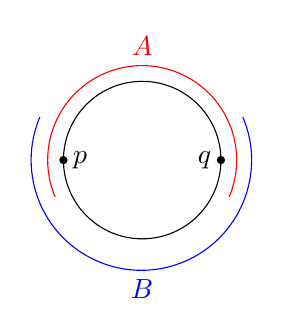
\begin{tikzpicture}
      \draw circle [radius=1];
      \draw [red] (1.105, -0.4673) arc(-22.9:202.9:1.2);
      \node [red, above] at (0, 1.2) {$A$};

      \draw [blue] (1.279, 0.545) arc(22.9:-202.9:1.4);
      \node [blue, below] at (0, -1.4) {$B$};

      \node [circ] at (1, 0) {};
      \node at (1, 0) [left] {$q$};
      \node [circ] at (-1, 0) {};
      \node at (-1, 0) [right] {$p$};
    \end{tikzpicture}
  \end{center}
  We want to apply Mayer-Vietoris. We have
  \[
    A \cong B \cong \R \simeq *,\quad A \cap B \cong \R \coprod \R \simeq \{p\} \coprod \{q\}.
  \]
  We obtain
  \[
    \begin{tikzcd}
      \cdots \ar[r] & H_1(A \cap B) \ar[r] & H_1(A) \oplus H_1(B) \ar[r] & H_1(S^1)\ar[out=0, in=180, looseness=2, overlay, lld]\\
      & H_0(A \cap B) \ar[r, "i_{A*} \oplus i_{B*}"] & H_0(A) \oplus H_0(B) \ar[r] & H_0(S^1) \ar [r] & 0
    \end{tikzcd}
  \]
  We replace these with the known objects to get
  \[
    \begin{tikzcd}
      \cdots \ar[r] & 0 \ar[r] & 0 \ar[r] & H_1(S^1)\ar[out=0, in=180, looseness=2, overlay, lld, "f"]\\
      & \Z \oplus \Z \ar[r, "g"] & \Z \oplus \Z \ar[r] & \Z \ar [r] & 0
    \end{tikzcd}
  \]
  We can now try to figure out what the maps are. We know that $H_0(A \cap B) \cong \Z \oplus \Z$ is generated by $p$ and $q$, and the inclusion map sends each of $p$ and $q$ to the unique connected components of $A$ and $B$. So the homology classes are both sent to $(1, 1) \in H_0(A) \oplus H_0(B) \cong \Z \oplus \Z$. We then see that the kernel of $g$ is generated by $(p - q)$, and is thus isomorphic to $\Z$.

  Since the map into $H_1(S^1)$ is from $0$, it has trivial image. So the map $f$ must be injective by exactness. So $H_1(S^1)$ is isomorphic to its image in $H_0(A \cap B)$ The image of $f$ is the kernel of $g$, and is thus isomorphic to $\Z$.

  By looking higher up the exact sequence, we see that all other homology groups vanish.
\end{eg}

We can do the sphere in general in the same way.

\begin{thm}
  For any $n \geq 1$, we have
  \[
    H_i(S^n) =
    \begin{cases}
      \Z & i = 0, n\\
      0 & \text{otherwise}
    \end{cases}.
  \]
\end{thm}

\begin{proof}
  We cut up $^n$ as
  \begin{align*}
    A &= S^n \setminus \{N\} \cong \R^n \simeq *,\\
    B &= S^n \setminus \{S\} \cong \R^n \simeq *,
  \end{align*}
  where $N$ and $S$ are the north and south poles. Moreover, we have
  \[
    A\cap B \cong \R \times S^{n - 1} \simeq S^{n - 1}
  \]
  So we can ``induct up'' using the Mayer-Vietoris sequence:
  \[
    \begin{tikzcd}
      \cdots \ar[r] & H_i(S^{n - 1}) \ar[r] & H_i(*) \oplus H_i(*) \ar[r] & H_i(S^n)\ar[out=0, in=180, looseness=2, overlay, lld, "\partial"]\\
      & H_{i - 1}(S^{n - 1}) \ar[r] & H_{i - 1}(*) \oplus H_{i - 1}(*) \ar[r] & H_{i - 1}(S^n) \ar [r] & \cdots
    \end{tikzcd}
  \]
  Now suppose $n \geq 2$, as we already did $S^1$ already. If $i > 1$, then $H_1(*) = 0 = H_{i - 1}(*)$. So the Mayer-Vietoris map
  \[
    \begin{tikzcd}
      H_i(S^n) \ar[r, "\partial"] & H_{i - 1}(S^{n - 1})
    \end{tikzcd}
  \]
  is an isomorphism.

  All that remains is to look at $i = 0, 1$. The $i = 0$ case is trivial. For $i = 1$, we look at
  \[
    \begin{tikzcd}
      & \cdots \ar[r] & H_1(*) \oplus H_1(*) \ar[r] & H_1(S^n)\ar[out=0, in=180, looseness=2, overlay, lld, "\partial"]\\
      & H_0(S^{n - 1}) \ar[r] & H_0(*) \oplus H_0(*) \ar[r] & H_0(S^n) \ar [r] & 0
    \end{tikzcd}
  \]
  Again, we plug in the known values to obtain
  \[
    \begin{tikzcd}
      & \cdots \ar[r] & 0 \ar[r] & H_1(S^n)\ar[out=0, in=180, looseness=2, overlay, lld]\\
      & \Z \ar[r, "f"] & \Z \oplus \Z \ar[r] & \Z \ar [r] & 0
    \end{tikzcd}
  \]
  To conclude that $H_1(S^n)$ is trivial, it suffices to show that the map $f$ is injective. But picking the canonical generators, it is given by $1 \mapsto (1, 1)$.
\end{proof}
While we know what the groups are, it is difficult for us to figure out what the generators of the groups are, since we need to trace through lots of Mayer-Vietoris homomorphisms. Later, we will develop cellular homology, which will make this much easier.

\begin{cor}
  If $n \not= m$, then $S^{n - 1} \not\simeq S^{m - 1}$, since they have different homology groups.
\end{cor}

\begin{cor}
  If $n \not= m$, then $\R^n \not \cong \R^m$.
\end{cor}

We can also use homology to define a useful notion.
\begin{defi}[Degree of a map]\index{degree of map}
  Let $f: S^n \to S^n$ be a map. Then we obtain a map $f_*: H_n(S^n) \to H_n(S^n)$. But we know $H_n(S^n) \cong \Z$. We know that any map from $\Z$ to itself is multiplication by an integer, which we call the \emph{degree} of $f$, written $\deg(f)$.
\end{defi}

In particular, for $n = 1$, the degree is the winding number.

Elementary properties of the degree follows from properties of homology.
\begin{prop}\leavevmode
  \begin{enumerate}
    \item $\deg(\id_{S^n}) = 1$.
    \item If $f$ is not surjective, then $\deg(f) = 0$.
    \item We have $\deg(f\circ g) = (\deg f)(\deg g)$.
    \item Homotopic maps have equal degrees.
  \end{enumerate}
\end{prop}

\begin{proof}\leavevmode
  \begin{enumerate}
    \item Obvious.
    \item If $f$ is not surjective, then $f$ can be factored as
      \[
        \begin{tikzcd}
          S^n \ar[r, "f"] & S^n \setminus \{p\} \ar[r, hook] & S^n
        \end{tikzcd},
      \]
      where $p$ is some point not in the image of $f$. But $S^n \setminus \{p\}$ is contractible. So $f_*$ factors as
      \[
        \begin{tikzcd}
          f_*: H_n(S^n) \ar[r] & H_n(*) = 0 \ar[r] & H_n(S^n)
        \end{tikzcd}.
      \]
      So $f_*$ is the zero homomorphism, and is thus multiplication by $0$.
    \item This follows from the functoriality of $H_n$.
    \item Obvious as well.
  \end{enumerate}
\end{proof}

\begin{cor}[Brouwer's fixed point theorem]\index{Brouwer's fixed point theorem}
  any map $f: D^n \to D^n$ has a fixed point.\term{fixed point}
\end{cor}

\begin{proof}
  Suppose $f$ has no fixed point. Define $r: D^n \to S^{n - 1} = \partial D^n$ by taking the intersection of the ray from $f(x)$ through $x$ with $\partial D^n$. This is continuous.
  \begin{center}
    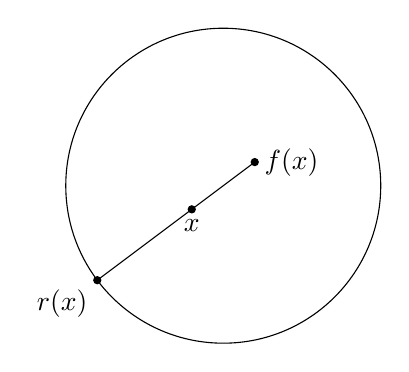
\begin{tikzpicture}
      \draw circle [radius=2cm];
      \node [circ] at (-0.4, -0.3) {};
      \node at (-0.4, -0.3) [below] {$x$};

      \node [circ] at (0.4, 0.3) {};
      \node at (0.4, 0.3) [right] {$f(x)$};
      \draw (0.4, 0.3) -- (-1.6, -1.2);
      \node at (-1.6, -1.2) [circ] {};
      \node at (-1.6, -1.2) [anchor = north east] {$r(x)$};
    \end{tikzpicture}
  \end{center}
  Now if $x \in \partial D^n$, then $r(x) = x$. So we have
  \[
    \begin{tikzcd}
      S^{n - 1} = \partial D^n \ar[r, "i"] & D^n \ar[r, "S^{n - 1}"] & \partial D^n = S^{n - 1}
    \end{tikzcd},
  \]
  and the composition is the identity. This is a contradiction --- contracting $D^n$ to a point, this gives a homotopy from the identity map $S^{n - 1} \to S^{n - 1}$ to the constant map at a point. This is impossible, as the two maps have different degrees.
\end{proof}
A more manual argument to show this would be to apply $H_{n - 1}$ to the chain of maps above to obtain a contradiction.

We know there is a map of degree $1$, namely the identity, and a map of degree $0$, namely the constant map. How about other degrees?

\begin{prop}
  A reflection $r: S^n \to S^n$ about a hyperplane has degree $-1$. As before, we cover $S^n$ by
  \begin{align*}
    A &= S^n \setminus \{N\} \cong \R^n \simeq *,\\
    B &= S^n \setminus \{S\} \cong \R^n \simeq *,
  \end{align*}
  where we suppose the north and south poles lie in the hyperplane of reflection. Then both $A$ and $B$ are invariant under the reflection. Consider the diagram
  \[
    \begin{tikzcd}
      H_n(S^n) \ar[r, "\partial_{MV}", "\sim"'] \ar[d, "r_*"] & H_{n - 1}(A \cap B) \ar[d, "r_*"] & H_{n - 1}(S^{n - 1}) \ar[l, "\sim"] \ar[d, "r_*"]\\
      H_n(S^n) \ar[r, "\partial_{MV}", "\sim"'] & H_{n - 1}(A \cap B) & H_{n - 1}(S^{n - 1}) \ar[l, "\sim"]
    \end{tikzcd}
  \]
  where the $S^{n - 1}$ on the right most column is given by contracting $A \cap B$ to the equator. Note that $r$ restricts to a reflection on the equation. By tracing through the isomorphisms, we see that $\deg(r) = \deg(r|_{\mathrm{equator}})$. So by induction, we only have to consider the case when $n = 1$. Then we have
  \[
    \begin{tikzcd}
      0 \ar[r] & H_1(S^1) \ar[r, "\partial_{MV}", "\sim"'] \ar[d, "r_*"] & H_0(A \cap B) \ar[d, "r_*"] \ar[r] & H_0(A) \oplus H_0(B) \ar[d, "r_* \oplus r_*"]\\
      0 \ar[r] & H_1(S^1) \ar[r, "\partial_{MV}", "\sim"'] & H_0(A \cap B) \ar[r] & H_0(A) \oplus H_0(B)
    \end{tikzcd}
  \]
  Now the middle vertical map sends $p \mapsto q$ and $q \mapsto p$. Since $H_1(S^1)$ is given by the kernel of $H_0(A \cap B) \to H_0(A) \oplus H_0(B)$, and is generated by $p - q$, we see that this sends the generator to its negation. So this is given by multiplication by $-1$. So the degree is $-1$.
\end{prop}

\begin{cor}
  The antipodal map $a: S^n \to S^n$ given by
  \[
    a(x_1, \cdots, x_{n + 1}) = (-x_1, \cdots, -x_n)
  \]
  has degree $(-1)^{n + 1}$ because it is a composition of $(n + 1)$ reflections.
\end{cor}

\begin{cor}[Hairy ball theorem]\index{Hairy ball theorem}
  $S^n$ has a nowhere $0$ vector field iff $n$ is odd.
\end{cor}

\begin{proof}
  Viewing $S^n \subseteq \R^{n + 1}$, a vector field on $S^n$ is a function $v: S^n \to \R^{n + 1}$ such that $\bra v(x), x\ket = 0$, ie. $v(x)$ is perpendicular to $x$.

  If $n$ is odd, say $n = 2k - 1$, then
  \[
    v(x_1, y_1, x_2, y_2, \cdots, x_k, y_k) = (y_1, -x_1, y_2, -x_2, \cdots, y_k, -x_k)
  \]
  works.

  Conversely, if $v: S^n \to \R^{n + 1} \setminus \{0\}$ is a vector field, we let $w = \frac{v}{\abs{v}}: S^n \to S^n$. We can construct a homotopy from $w$ to the antipodal map by ``linear interpolation'', but in a way so that it stays on the sphere. We let
  \begin{align*}
    H: [0, \pi] \times S^n &\to S^n\\
    (t, x) &\mapsto \cos(t) x + \sin(t) w(x)
  \end{align*}
  Since $w(x)$ and $x$ are perpendicular, it follows that this always has norm $1$, so indeed it stays on the sphere.

  Now we have
  \[
    H(0, x) = x,\quad H(\pi, x) = -x.
  \]
  So this gives a homotopy from $\id$ to $a$, which is a contradiction since they have different degrees.
\end{proof}


\begin{eg}
  Let $K$ be the Klein bottle. We cut them up by
  \begin{center}
    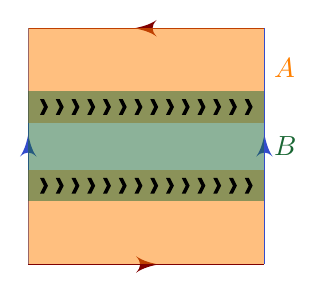
\begin{tikzpicture}
      \draw [->-=0.55, mred] (0, 0) -- (3, 0);
      \draw [->-=0.55, mred] (3, 3) -- (0, 3);
      \draw [->-=0.55, mblue] (3, 0) -- (3, 3);
      \draw [->-=0.55, mblue] (0, 0) -- (0, 3);

      \fill [morange, opacity=0.5] (0, 0) rectangle (3, 1.2);
      \fill [morange, opacity=0.5] (0, 1.8) rectangle (3, 3);
      \node [right, morange] at (3, 2.5) {$A$};

      \fill [mgreen, opacity=0.5] (0, 0.8) rectangle (3, 2.2);
      \node [right, mgreen] at (3, 1.5) {$B$};

      \foreach \n in {0,1,2,3,4,5,6,7,8,9,10,11,12,13} {
        \begin{scope}[shift={(0.15 + 0.2 * \n, 0.9)}]
          \fill (0, 0) -- (0.05, 0) -- (0.1, 0.1) -- (0.05, 0.2) -- (0, 0.2) -- (0.05, 0.1) -- cycle;
        \end{scope}

        \begin{scope}[shift={(0.15 + 0.2 * \n, 1.9)}]
          \fill (0, 0) -- (0.05, 0) -- (0.1, 0.1) -- (0.05, 0.2) -- (0, 0.2) -- (0.05, 0.1) -- cycle;
        \end{scope}
      }
    \end{tikzpicture}
  \end{center}
  Then both $A$ and $B$ are cylinders, and their intersection is two cylinders:
  \begin{center}
    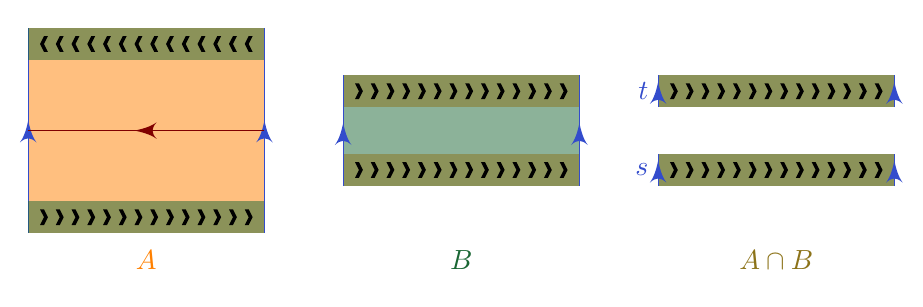
\begin{tikzpicture}
      \fill [morange, opacity=0.5] (0, 0) rectangle (3, 2.6);
      \draw [->-=0.55, mblue] (3, 0) -- (3, 2.6);
      \draw [->-=0.55, mblue] (0, 0) -- (0, 2.6);
      \draw [->-=0.55, mred] (3, 1.3) -- (0, 1.3);
      \fill [mgreen, opacity=0.5] (0, 0) rectangle (3, 0.4);
      \fill [mgreen, opacity=0.5] (0, 2.2) rectangle (3, 2.6);

      \foreach \n in {0,1,2,3,4,5,6,7,8,9,10,11,12,13} {
        \begin{scope}[shift={(0.15 + 0.2 * \n, 0.1)}]
          \fill (0, 0) -- (0.05, 0) -- (0.1, 0.1) -- (0.05, 0.2) -- (0, 0.2) -- (0.05, 0.1) -- cycle;
        \end{scope}

        \begin{scope}[shift={(0.2 + 0.2 * \n, 2.3)}]
          \fill (0, 0) -- (0.05, 0) -- (0, 0.1) -- (0.05, 0.2) -- (0, 0.2) -- (-0.05, 0.1) -- cycle;
        \end{scope}
      }
      \node at (1.5, -0.1) [morange, below] {$A$};

      \fill [morange, opacity=0.5] (4, 0.6) rectangle (7, 1);
      \fill [morange, opacity=0.5] (4, 1.6) rectangle (7, 2);
      \fill [mgreen, opacity=0.5] (4, 0.6) rectangle (7, 2);
      \draw [->-=0.57, mblue] (4, 0.6) -- (4, 2);
      \draw [->-=0.57, mblue] (7, 0.6) -- (7, 2);

      \foreach \n in {0,1,2,3,4,5,6,7,8,9,10,11,12,13} {
        \begin{scope}[shift={(4.15 + 0.2 * \n, 0.7)}]
          \fill (0, 0) -- (0.05, 0) -- (0.1, 0.1) -- (0.05, 0.2) -- (0, 0.2) -- (0.05, 0.1) -- cycle;
        \end{scope}

        \begin{scope}[shift={(4.15 + 0.2 * \n, 1.7)}]
          \fill (0, 0) -- (0.05, 0) -- (0.1, 0.1) -- (0.05, 0.2) -- (0, 0.2) -- (0.05, 0.1) -- cycle;
        \end{scope}
      }

      \node at (5.5, -0.1) [mgreen, below] {$B$};

      \begin{scope}[shift={(4, 0)}]
        \fill [morange, opacity=0.5] (4, 0.6) rectangle (7, 1);
        \fill [morange, opacity=0.5] (4, 1.6) rectangle (7, 2);
        \fill [mgreen, opacity=0.5] (4, 0.6) rectangle (7, 1);
        \fill [mgreen, opacity=0.5] (4, 1.6) rectangle (7, 2);
        \draw [->-=0.8, mblue] (4, 0.6) -- (4, 1) node [left, pos=0.5] {$s$};
        \draw [->-=0.8, mblue] (7, 0.6) -- (7, 1);
        \draw [->-=0.8, mblue] (4, 1.6) -- (4, 2) node [left, pos=0.5] {$t$};
        \draw [->-=0.8, mblue] (7, 1.6) -- (7, 2);

        \foreach \n in {0,1,2,3,4,5,6,7,8,9,10,11,12,13} {
          \begin{scope}[shift={(4.15 + 0.2 * \n, 0.7)}]
            \fill (0, 0) -- (0.05, 0) -- (0.1, 0.1) -- (0.05, 0.2) -- (0, 0.2) -- (0.05, 0.1) -- cycle;
          \end{scope}

          \begin{scope}[shift={(4.15 + 0.2 * \n, 1.7)}]
            \fill (0, 0) -- (0.05, 0) -- (0.1, 0.1) -- (0.05, 0.2) -- (0, 0.2) -- (0.05, 0.1) -- cycle;
          \end{scope}
        }

        \node at (5.5, -0.1) [mgreen!50!morange, below] {$A \cap B$};
      \end{scope}
    \end{tikzpicture}
  \end{center}
  We have a long exact sequence
  \[
    \begin{tikzcd}
      0 \ar[r] & H_2(K) \ar[r] & H_1(A \cap B) \ar[r, "{(i_A, i_B)}"] & H_1(A) \oplus H_1(B) \ar[r, "j_A - j_B"] & \vphantom{0}\\
      & H_1(K) \ar[r] & H_0(A \cap B) \ar[r, "{(i_A, i_B)}"] & H_0(A) \oplus H_0(B) \ar[r, "j_A - j_B"] & \vphantom{0}\\
      & H_0(K) \ar[r] & 0
    \end{tikzcd}
  \]
  We plug in the numbers to get
  \[
    \begin{tikzcd}
      0 \ar[r] & H_2(K) \ar[r] & \Z \oplus \Z \ar[r, "{(i_A, i_B)}"] & \Z \oplus \Z \ar[r, "j_A - j_B"] & \vphantom{0}\\
      & H_1(K) \ar[r] & \Z \oplus \Z \ar[r, "{(i_A, i_B)}"] & \Z \oplus \Z \ar[r, "j_A - j_B"] & \Z \ar[r] & 0
    \end{tikzcd}
  \]
  Now let's look at the first $(i_A, i_B)$ map. We suppose each $H_1$ is generated by the left-to-right loops. Then we have
  \begin{align*}
    i_A(s) &= -1\\
    i_A(t) &= 1\\
    i_B(s) &= 1\\
    i_B(s) &= 1
  \end{align*}
  So the matrix of $(i_A, i_B)$ is
  \[
    \begin{pmatrix}
      -1 & 1\\
      1 & 1
    \end{pmatrix}.
  \]
  This has determinant $2$, so it is injective and has trivial kernel. So we must have $H_2(K) = 0$. We also have
  \[
    \frac{H_1(A) \oplus H_1(B)}{\im(i_A, i_B)} = \frac{\bra a, b\ket}{\bra -a + b, a + b\ket} \frac{\bra a\ket}{\bra 2a\ket} \cong \Z/2\Z.
  \]
  Now the the second $(i_A, i_B)$ is given by
  \[
    \begin{pmatrix}
      1 & 1\\
      1 & 1
    \end{pmatrix},
  \]
  which is isomorphic to $\Z$. So we have
  \[
    \begin{tikzcd}
      0 \ar[r] & \Z/2\Z \ar[r] & H_1(K) \ar[r] & \Z \ar[r] & 0
    \end{tikzcd}.
  \]
  So we have $H_1(K) \cong \Z \oplus \Z/2\Z$.

  % explain better
\end{eg}

We are now going to give an application of excision to compute degrees.

\begin{lemma}
  Let $M$ be a $d$-dimensional manifold (ie. a Hausdorff, second-countable space locally homeomorphic to $\R^d$). Then
  \[
    H_n(M, M \setminus x) \cong
    \begin{cases}
      \Z & n = d\\
      0 & \text{otherwise}
    \end{cases}.
  \]
  This is known as the \term{local homology}
\end{lemma}
This gives us a homological way to define the dimension of a space.

\begin{proof}
  Let $U$ be an open neighbourhood isomorphic to $\R^d$ that maps $x \mapsto 0$. We let $\Z = M\setminus U$. Then
  \[
    \overline{Z} = Z \subseteq M \setminus \{x\} = \mathring{(M \setminus \{x\})}.
  \]
  So we can apply excision, and get
  \[
    H_n(U, U \setminus \{x\}) = H_n(M\setminus Z, (M\setminus \{x\})\setminus \Z) \cong H_n(M, M\setminus X).
  \]
  Using the fact that $U \cong \R^d \simeq *$ and $\R^d \setminus \{0\} \simeq S^{d - 1}$, the long exact sequence for relative homology gives the result.
\end{proof}

Now let $f: S^d \to S^d$ be a map. Suppose there is a $y \in S^d$ such that
\[
  f^{-1}(y) = \{x_1, \cdots, x_k\}
\]
is finite. We choose an open enighbourhood $V$ of $y$, and open neighbourhoods $U_i$ of $x_i$ such that
\begin{enumerate}
  \item $U_i \cap U_j = \emptyset$ for $i \not= j$.
  \item $f(U_i) \subseteq V$.
\end{enumerate}
We have a map
\[
  \begin{tikzcd}
    H_d(U_i, U_i \setminus \{x\}) \ar[r, "(f|_{U_i})_*"] & H_d(V, V \setminus \{y\})
  \end{tikzcd},
\]
and we know each object is isomorphic to $\Z$. So the map is multiplication by some integer, and we want to call that the degree. However, we have to be careful how we identify each object with $\Z$, or else the degree is only well-defined up to a sign.

So we consider the maps
\[
  \begin{tikzcd}
    H_d(U_i, U_i \setminus \{x\}) \ar[r, "(f|_{U_i})_*"] \ar[d, "i"] & H_d(V, V \setminus \{y\}) \ar[d, "i"]\\
    H_d(S^d, S^d\setminus\{x_i\}) \ar[d] & H_d(S^d, S^d\setminus\{x_i\}) \ar[d]\\
    H_d(S^d) & H_d(S^d)
  \end{tikzcd}
\]
All the maps shown are canonically defined. So as long as we are consistent in how we identify $H_d(S^d)$ with $\Z$, we have a well-defined degree, called the \emph{local degree}, written $\deg(f)_{x_i}$.

\begin{thm}
  Let $f: S^d \to S^d$ be a map. Suppose there is a $y \in S^d$ such that
  \[
    f^{-1}(y) = \{x_1, \cdots, x_k\}
  \]
  is finite. Then
  \[
    \deg (f) = \sum_{i = 1}^k \deg(f)_{x_i}.
  \]
\end{thm}

\begin{proof}
  \[
    \begin{tikzcd}
      H_d(S^d) \ar[r, "f_*"] \ar[d] & H_d(S^d) \ar[d, "\sim"] & 1 \ar[r, maps to] \ar[ddd, maps to]& \deg(f) \ar[ddd, maps to]\\
      H_d(S^d, S^d \setminus \{x_1, \cdots, x_k\}) \ar[r, "f_*"] & H_d(S^d, S^d \setminus \{y\})\\
      H_d\left(\coprod U_i, \coprod (U_i \setminus x_i)\right) \ar[u, "\text{excision}"]\\
      \bigoplus_{i = 1}^ k H_d(U_i, U_i \setminus x_i) \ar[r, "\bigoplus f_*"] \ar[u, "\sim"] & H_d(V, V\setminus \{y\}) \ar[uu, "\sim"] & (1, \cdots, 1) \ar[r, maps to] & \sum_{i = 1}^k \deg(f)_{x_i}
    \end{tikzcd}
  \]
\end{proof}
\subsection{Repaying the technical debt}
We are now going to prove the theorems!

\subsubsection*{Long exact sequence of relative homology}
Let $A \subseteq X$ , and let $C_{\Cdot}(X, A) = C_{\Cdot}(X)/C_{\Cdot}(A)$. The long exact sequence on homology relates $H_{\Cdot}(A), H_{\Cdot}(X)$ and $H_{\Cdot}(X, A)$.

This is in fact a completely general theorem.
\begin{thm}[Snake lemma]\index{snake lemma}
  Suppose we have a short exact sequence of complexes
  \[
    \begin{tikzcd}
      0 \ar[r] & A_{\Cdot} \ar [r, "i_{\Cdot}"] & B_{\Cdot} \ar [r, "q_{\Cdot}"] & C_{\Cdot} \ar[r] & 0
    \end{tikzcd}.
  \]
  Then there are maps
  \[
    \partial: H_n(C_{\Cdot}) \to H_{n - 1}(A_{\Cdot})
  \]
  such that there is a long exact sequence
  \[
    \begin{tikzcd}
      \cdots \ar [r] & H_n(A) \ar[r, "i_*"] & H_n(B) \ar[r, "q_*"] & H_n(C) \ar[out=0, in=180, looseness=2, overlay, dll, "\partial_*"']\\
      & H_{n - 1}(A) \ar[r, "i_*"] & H_{n - 1}(B) \ar[r, "q_*"] & H_{n - 1}(C) \ar [r] & \cdots
    \end{tikzcd}.
  \]
\end{thm}
The method of proving this is sometimes known as ``diagram chasing'', where we just ``chase'' around commutative diagrams to find the elements we need. The idea of the proof is as follows --- in the short exact sequence, we can think of $A$ as a subgroup of $B$, and $C$ as the quotient $B/A$, by the first isomorphism theorem. So any element of $C$ can be represented by an element of $B$. We apply the boundary map to this representative, and then exactness shows that this must come from some element of $A$. We then check carefully that these is well-defined, ie. does not depend on the representatives chosen.

\begin{proof}
  The proof of this is in general not hard. It just involves a lot of checking of the details, such as making sure the homomorphisms are well-defined, are actually homomorphisms, are exact at all the places etc. The only important and non-trivial part is just the construction of the map $\partial_*$.

  First we look at the following commutative diagram:
  \[
    \begin{tikzcd}
      0 \ar[r] & A_n \ar[r, "i_n"] \ar[d, "d_n"] & B_n \ar[r, "q_n"] \ar[d, "d_n"] & C_n \ar[r] \ar[d, "d_n"] & 0\\
      0 \ar[r] & A_{n - 1} \ar[r, "i_{n - 1}"] & B_{n - 1} \ar[r, "q_{n - 1}"] & C_{n - 1} \ar[r] & 0
    \end{tikzcd}
  \]
  To construct $\partial_*: H_n(C) \to H_{n - 1}(A)$, let $[x] \in H_n(C)$ be a class represented by $x \in Z_n(C)$. We need to find a cycle $z \in A_{n - 1}$. By exactness, we know the map $q_n: B_n \to C_n$ is surjective. So there is a $y \in B_n$ such that $q_n(y) = x$. Since our target is $A_{n - 1}$, we want to move down to the next level. So consider $d_n(y) \in B_{n - 1}$. We would be done if $d_n(y)$ is in the image of $i_{n - 1}$. By exactness, this is equivalent saying $d_n(y)$ is in the kernel of $q_{n -1 }$. Since the diagram is commutative, we know
  \[
    q_{n - 1}\circ d_n(y) = d_n \circ q_n (y) = d_n(x) = 0,
  \]
  using the fact that $x$ is a cycle. So $d_n (y) \in \ker q_{n - 1} = \im i_{n - 1}$. Moreover, by exactness again, $i_{n - 1}$ is injective. So there is a unique $z \in A_{n - 1}$ such that $i_{n - 1}(z) = d_n(y)$. We have now produced our $z$.

  We are not done. We have $\partial_* [x] = [z]$ as our candidate definition, but we need to check many things:
  \begin{enumerate}
    \item We need to make sure $\partial_*$ is indeed a homomorphism.
    \item We need $d_{n - 1}(z) = 0$ so that $[z] \in H_{n - 1}(A)$;
    \item We need to check $[z]$ is well-defined, ie. it does not depend on our choice of $y$ and $x$ for the homology class $[x]$.
    \item We need to check the exactness of the resulting sequence.
  \end{enumerate}
  We now check them one by one:
  \begin{enumerate}
    \item Since everything involved in defining $\partial_*$ are homomorphisms, it follows that $\partial_*$ is also a homomorphism.
    \item We check $d_{n - 1}(z) = 0$. To do so, we need to add an additional layer.
      \[
        \begin{tikzcd}
          0 \ar[r] & A_n \ar[r, "i_n"] \ar[d, "d_n"] & B_n \ar[r, "q_n"] \ar[d, "d_n"] & C_n \ar[r] \ar[d, "d_n"] & 0\\
          0 \ar[r] & A_{n - 1} \ar[r, "i_{n - 1}"] \ar[d, "d_{n - 1}"] & B_n \ar[r, "q_{n - 1}"] \ar[d, "d_{n - 1}"] & C_n \ar[r] \ar[d, "d_{n - 1}"] & 0\\
          0 \ar[r] & A_{n - 2} \ar[r, "i_{n - 2}"] & B_{n - 2} \ar[r, "q_{n - 2}"] & C_{n - 2} \ar[r] & 0
        \end{tikzcd}
      \]
      We want to check that $d_{n - 1}(z) = 0$. We will use the commutativity of the diagram. In particular, we know
      \[
        i_{n - 2} \circ d_{n - 1}(z) = d_{n - 1} \circ i_{n - 1} (z) = d_{n - 1} \circ d_n(y) = 0.
      \]
      By exactness at $A_{n - 2}$, we know $i_{n - 2}$ is injective. So we must have $d_{n - 1}(z) = 0$.
    \item
      \begin{enumerate}
        \item First, in the proof, suppose we picked a different $y'$ such that $q_n(y') = q_n(y) = x$. Then $q_n(y' - y) = 0$. So $y' - y \in \ker q_n = \im i_n$. Let $a \in A_n$ be such that $i_n(a) = y' - y$. Then
          \begin{align*}
            d_n(y') &= d_n(y' - y) + d_n(y) \\
            &= d_n \circ i_n (a) + d_n(y) \\
            &= i_{n - 1} \circ d_n (a) + d_n(y).
          \end{align*}
          Hence when we pull back $d_n(y')$ and $d_n(y)$ to $A_{n - 1}$, the results differ by the boundary $d_n(a)$, and hence produce the same homology class.
        \item Suppose $[x'] = [x]$. We want to show that $\partial_* [x] = \partial_*[x']$. This time, we add a layer above.
          \[
            \begin{tikzcd}
              0 \ar[r] & A_{n + 1} \ar[r, "i_{n + 1}"] \ar[d, "d_{n + 1}"] & B_{n + 1} \ar[r, "q_{n + 1}"] \ar[d, "d_{n + 1}"] & C_{n + 1} \ar[r] \ar[d, "d_{n + 1}"] & 0\\
              0 \ar[r] & A_n \ar[r, "i_n"] \ar[d, "d_n"] & B_n \ar[r, "q_n"] \ar[d, "d_n"] & C_n \ar[r] \ar[d, "d_n"] & 0\\
              0 \ar[r] & A_{n - 1} \ar[r, "i_{n - 1}"] & B_{n - 1} \ar[r, "q_{n - 1}"] & C_{n - 1} \ar[r] & 0
            \end{tikzcd}
          \]
          By definition, since $[x'] = [x]$, there is some $c \in C_{n + 1}$ such that
          \[
            x' = x + d_{n + 1} (c).
          \]
          By surjectivity of $q_{n + 1}$, we can write $c = q_{n + 1}(b)$ for some $b \in B_{n + 1}$. By commutativity of the squares, we know
          \[
            x' = x + q_n \circ d_{n + 1} (b).
          \]
          The next step of the proof is to find some $y$ such that $q_n (y) = x$. Then
          \[
            q_n(y + d_{n + 1} (b)) = x'.
          \]
          So the corresponding $y'$ is $y' = y + d_{n + 1}(b)$. So $d_n (y) = d_n(y')$, and hence $\partial_*[x] = \partial_* [x']$.
      \end{enumerate}
    \item This is yet another standard diagram chasing argument. When reading this, it is helpful to look at a diagram and see how the elements are chased along. It is even more beneficial to attempt to prove this yourself.
      \begin{enumerate}
        \item $\im i_* \subseteq \ker q_*$: This follows from the assumption that $i_n \circ q_n = 0$.
        \item $\ker q_* \subseteq \im i_*$: Let $[b] \in H_n(B)$. Suppose $q_*([b]) = 0$. Then there is some $c \in C_{n + 1}$ such that $q_n(b) = d_{n + 1}(c)$. By surjectivity of $q_{n + 1}$, there is some $b' \in B_{n + 1}$ such that $q_{n + 1}(b') = c$. By commutativity, we know $q_n(b) = q_n \circ d_{n + 1}(b')$, ie.
          \[
            q_n (b - d_{n + 1}(b')) = 0.
          \]
          By exactness of the sequence, we know there is some $a \in A_n$ such that
          \[
            i_n(a) = b - d_{n + 1}(b').
          \]
          Moreover,
          \[
            i_{n - 1} \circ d_n(a) = d_n \circ i_n (a) = d_n(b - d_{n + 1}(b')) = 0,
          \]
          using the fact that $b$ is a cycle. Since $i_{n - 1}$ is injective, it follows that $d_n(a) = 0$. So $[a] \in H_n(A)$. Then
          \[
            i_*([a]) = [b] - [d_{n + 1}(b')] = [b].
          \]
          So $[b] \in \im i_*$.
        \item $\im q_* \subseteq \ker \partial_*$: Let $[b] \in H_n(B)$. To compute $\partial_*(q_*([b]))$, we first pull back $q_n(b)$ to $b \in B_n$. Then we compute $d_n(b)$ and then pull it back to $A_{n + 1}$. However, we know $d_n(b) = 0$ since $b$ is a cycle. So $\partial_*(q_*([b])) = 0$, ie. $\partial_* \circ q_* = 0$.
        \item $\ker \partial_* \subseteq \im q_*$: Let $[c] \in H_n(C)$ and suppose $\partial_*([c]) = 0$. Let $b \in B_n$ be such that $q_n(b) = c$, and $a \in A_{n - 1}$ such that $i_{n - 1}(a) = d_n(b)$. By assumption, $\partial_*([c]) = [a] = 0$. So we know $a$ is a boundary, say $a = d_n (a')$ for some $a' \in A_n$. Then by commutativity we know $d_n(b) = d_n \circ i_n (a')$. In other words,
          \[
            d_n(b - i_n(a')) = 0.
          \]
          So $[b - i_n(a')] \in H_n(B)$. Moreover,
          \[
            q_*([b - i_n(a')]) = [q_n(b) - q_n \circ i_n(a')] = [c].
          \]
          So $[c] \in \im q_*$.
        \item $\im \partial_* \subseteq \ker i_*$: Let $[c] \in H_n(C)$. Let $b \in B_n$ be such that $q_n(b) = c$, and $a \in A_{n - 1}$ be such that $i_n(a) = d_n(b)$. Then $\partial_*([c]) = [a]$. Then
          \[
            i_*([a]) = [i_n(a)] = [d_n(b)] = 0.
          \]
          So $i_* \circ \partial_* = 0$.
        \item $\ker i_* \subseteq \im \partial_*$: Let $[a] \in H_n(A)$ and suppose $i_*([a]) = 0$. So we can find some $b \in B_{n + 1}$ such that $i_n(a) = d_{n + 1}(b)$. Let $c = q_{n + 1}(b)$. Then
          \[
            d_{n + 1}(c) = d_{n + 1}\circ q_{n + 1} (b) = q_n \circ d_{n + 1}(b) = q_n \circ i_n (a) = 0.
          \]
          So $[c] \in H_n(C)$. Then $[a] = \partial_*([c])$ by definition of $\partial_*$. So $[a] \in \im \partial_*$.
      \end{enumerate}
  \end{enumerate}
\end{proof}

Another piece of useful algebra is known as the $5$-lemma:
\begin{lemma}[Five lemma]
  Consider the following commutative diagram:
  \[
    \begin{tikzcd}
      A \ar[r, "f"] \ar[d, "\ell"] & B \ar[r, "g"] \ar[d, "m"] & C \ar[r, "h"] \ar[d, "n"] & D \ar[r, "j"] \ar[d, "p"] & E \ar[d, "q"]\\
      A' \ar[r, "r"] & B' \ar[r, "s"] & C' \ar[r, "t"] & D' \ar[r, "u"] & E'
    \end{tikzcd}
  \]
  If the two rows are exact, $m$ and $p$ are isomorphisms, $q$ is injective and $\ell$ is surjective, then $n$ is also an isomorphism.
\end{lemma}

\begin{proof}
  The philosophy is exactly the same as last time.

  We first show that $n$ is surjective. Let $c' \in C'$. Then we obtain $d' = t(c') \in D'$. Since $p$ is an isomorphism, we can find $d \in D$ such that $p(d) = d'$. Then we have
  \[
    q(j(d)) = u(p(d)) = u(f(c')) = 0.
  \]
  Since $q$ is injective, we know $j(d) = 0$. Since the sequence is exact, there is some $c \in C$ such that $h(c) = d$.

  We are not yet done. We do not know that $n(c) = c'$. All we know is that $d(n(c)) = d(c')$. So $d(c' - n(c)) = 0$. By exactness at $C'$, we can find some $b'$ such that $s(b') = n(c) - c'$. Since $m$ was surjective, we can find $b \in B$ such that $m(b) = b'$. Then we have
  \[
    n(g(b)) = n(c) - c'.
  \]
  So we have
  \[
    n(c - g(b)) = c'.
  \]
  So $n$ is surjective.

  Showing that $n$ is injective is similar.
  % complete
\end{proof}

\begin{cor}
  Let $f: (X, A) \to (Y, B)$ be a map of pairs, and that any two fo $f_*: H_*(X, A) \to H_*(Y, B)$, $H_*(X) \to H_*(Y)$ and $H_*(A) \to H_*(B)$ are isomorphisms. Then the third is also an isomorphism.
\end{cor}

\begin{proof}
  Follows from the long exact sequence and the five lemma.
\end{proof}

\subsubsection*{Proof of homotopy invariance}

We want to show that homotopy of continuous maps does not affect the induced map on the homology groups. We will do this by showing that homotopies of maps induce homotopies of chain complexes, and chain homotopic maps induce the same map on homology groups.

\begin{defi}[Chain homotopy]\index{chain homotopy}
  A \emph{chain homotopy} between chain maps $f_{\Cdot}, g_{\Cdot}: C_{\Cdot} \to D_{\Cdot}$ is a collection of homomorphisms $F_n: C_n \to D_{n + 1}$ such that
  \[
    g_n - f_n = d_{n + 1}^D \circ F_n + F_{n - 1} \circ d_n^C: C_n \to D_n
  \]
  for all $n$.
\end{defi}

The relevance of this definition is the following result:
\begin{lemma}
  If $f_{\Cdot}$ and $g_{\Cdot}$ are chain homotopies, then $f_* = g_*: H_*(C_{\Cdot}) \to H_*(D_{\Cdot})$.
\end{lemma}

\begin{proof}
  Let $[c] \in H_n(C_{\Cdot})$. Then we have
  \[
    g_n(c) - f_n(c) = d_{n + 1}^Df_n(c) + F_{n - 1}(d_n^C(c)) = d_{n + 1}^Df_n(c),
  \]
  where the second term dies because $c$ is a cycle. So we have $[g_n(c)] = [f_n(c)]$.
\end{proof}

That was the easy part. What we need to do now is to show that homotopy of maps between spaces gives a chain homotopy between the corresponding chain maps.

\begin{notation}
  From now on, we will just write $d$ for $d_n^C$.

  For $f: X \to Y$, we will write $f_\#: C_n(X) \to C_n(Y)$ for the map $\sigma \mapsto f \circ \sigma$, ie. what we used to call $f_n$.
\end{notation}

Now if $H: [0, 1] \times X \to Y$ is a homotopy from $f$ to $g$, and $\sigma: \Delta^n \to X$ is an $n$-chain, then we get a homotopy
\[
  \begin{tikzcd}
    \lbrack0, 1\rbrack \times \Delta^n \ar[r, "{[0, 1] \times \sigma}"] & \lbrack0, 1\rbrack \times X \ar[r, "H"] & Y
  \end{tikzcd}
\]
from $f_\#(\sigma)$ to $g_\#(\sigma)$. Note that we write $[0, 1]$ for the identity map $[0, 1] \to [0, 1]$.


Suppose we can find a collection of chains $P_n \in C_{n + 1}([0, 1] \times \Delta^n)$ for $n \geq 0$ such that
\[
  d(P_n) = i_1 - i_0 - \sum_{j = 0}^n (-1)^j ([0, 1] \times \delta_j)_\#(P_{n - 1}),
\]
where
\begin{align*}
  i_0: \delta^n &= \{0\} \times \Delta^n \hookrightarrow [0, 1] \times \Delta^n\\
  i_1: \delta^n &= \{0\} \times \Delta^n \hookrightarrow [0, 1] \times \Delta^n
\end{align*}
and $\delta_j: \Delta^{n - 1} \to \Delta^n$ is the inclusion of the $j$th face.

We then define
\[
  F_n: C_n(X) \to C_{n + 1}(Y)
\]
by sending
\[
  (\sigma: \Delta^n \to X) \mapsto H \circ ([0, 1] \times \sigma)_\#(P_n).
\]
We now calculate.
\begin{align*}
  \d F_n(\sigma) ={}& d((H \circ (1 \times \Delta^n))_\#(P_n))\\
  ={}& (H \circ ([0, 1] \times \sigma))_\#(d(P_n))\\
  ={}& (H \circ ([0, 1] \times \sigma))_\# \left(i_1 - i_0 - \sum_{j = 0}^n (-1)^j ([0, 1] \times \delta_j)_\#(P_{n - 1})\right)\\
  ={}& H \circ ([0, 1] \times \sigma) \circ i_1 - H \circ ([0, 1] \times \sigma) \circ i_0 \\
  &\quad- \sum_{j = 0}^n (-1)^j H_\# \circ (([0, 1] \times \sigma) \circ \delta_j)_\# (P_{n - 1})\\
  ={}& g \circ \sigma - f \circ \sigma - \sum_{j = 0}^n (-1)^j H_\# \circ (([0, 1] \times \sigma) \circ \delta_j)_\# (P_{n - 1})\\
  ={}& g \circ \sigma - f \circ \sigma - F_{n - 1}(\d \sigma)\\
  ={}& g_\#(\sigma) - f_\#(\sigma) - F_{n - 1}(d\sigma).
\end{align*}
So we just have to show that $P_n$ exists. Morally, it is the ``prism'' obtained by dissecting $[0, 1] \times \Delta^n$ into a sum of simplices. This is rather hard to visualize, so let's just write down a formula and check that it works.

Consider $[0, 1] \times \Delta^n \in \R \times \R^{n + 1}$, where it is convex. Let $\{v_0, v_1, \cdots, v_n\}$ for the vertices of $\{0\} \times \Delta^n \subseteq [1, 0] \times \Delta^n$. We write $\{w_0, \cdots, w_n\}$ for the corresponding vertices of $\{1\} \times \Delta^n$.

Now if $\{x_0, x_1, \cdots, x_{n + 1}\} \subseteq \{v_0, \cdots, v_n\} \cup \{w_0, \cdots, w_n\}$, we let
\[
  [x_0, \cdots, x_n]: \Delta^n \to [0, 1] \times \Delta^n
\]
by
\[
  (t_0, \cdots, t_{n + 1}) = \sum t_i x_i.
\]
This is still in the space by convexity. We let
\[
  P_n = \sum_{i = 0}^n (-1)^i [v_0, v_1 , \cdots, v_i, w_i, w_{i + 1}, \cdots, w_n] \in C_{n + 1}([0, 1] \times \Delta^n).
\]
We can check that it works.

\subsubsection*{Proof of excision and Mayer-Vietoris}

It turns out the proofs of excision and Mayer-Vietoris are essentially the same thing, which we will call the ``small simplices theorem''.

We let $\mathcal{U} = \{U_\alpha\}_{\alpha \in I}$ be a collection of subspaces of $X$ such that their interiors cover $X$, ie.
\[
  \bigcup_{\alpha \in I} \mathring{U_\alpha} = X.
\]
\begin{defi}[$C_n^\mathcal{U}(X)$ and $H_n^\mathcal{U}(X)$]\index{$C_n^\mathcal{U} (X)$}\index{$H_n^\mathcal{U}(X)$}.
  Let $C_n^\mathcal{U}(X) \subseteq C_n(X)$ be the subgroup generated by those singular $n$-simplices $\sigma: \delta^n \to X$ such that $\sigma(\Delta^n) \subseteq U_\alpha$ for some $\alpha$. It is clear that if $\sigma$ lies in $U_\alpha$, then so do its faces. So $C_n^{\mathcal{U}}(X)$ is a sub-chain complex of $C_\Cdot(X)$.

  We write $H_n^\mathcal{U}(X) = H_n(C_\Cdot^\mathcal{U}(X))$.
\end{defi}
It would be annoying if each choice of open cover gives a different homology theory, because there are too many things to think about. The \emph{small simplices theorem} says that the natural map $H_*^\mathcal{U}(X) \to H_*(X)$ is an isomorphism.

\begin{thm}[Small simplices theorem]\index{small simplices theorem}
  The natural map $H_*^\mathcal{U}(X) \to H_*(X)$ is an isomorphism.
\end{thm}

The idea is that we can cut up each simplex into smaller parts by barycentric subdivision, and if we do it enough, it will eventually lie in on of the open covers. We then go on to prove that cutting it up does not change homology.

Proving it is not hard, but technically annoying. So we first use this to deduce our theorems.

\begin{proof}[Proof of Mayer-Vietoris]
  Let $X = A \cup B$, with $A, B$ open in $X$. We let $\mathcal{U} = \{A, B\}$, and write $C_\Cdot(A + B) = C_\Cdot^\mathcal{U} (X)$. Then we have a natural chain map
  \[
    \begin{tikzcd}
      C_\Cdot(A) \oplus C_{\Cdot}(B) \ar[r, "j_A - j_B"] & C_\Cdot(A + B)
    \end{tikzcd}
  \]
  that is surjective. The kernel consists of $(x, y)$ such that $j_A(x) - j_B(y) = 0$, ie. $j_A(x) = j_B(y)$. But $j$ doesn't really do anything. It just forgets that the simplices lie in $A$ or $B$. So this means $y = x$ is a chain in $A \cap B$. We thus deduce that we have a short exact sequence of chain complexes
  \[
    \begin{tikzcd}
      C_\Cdot(A \cap B) \ar[r, "{(i_A, i_B)}"] & C_\Cdot(A) \oplus C_{\Cdot}(B) \ar[r, "j_A - j_B"] & C_\Cdot(A + B).
    \end{tikzcd}
  \]
  Then the snake lemma shows that we obtain a long exact sequence of homology groups. So we get a long exact sequence of homology groups
  \[
    \begin{tikzcd}
      \cdots\ar[r] & H_n(A \cap B) \ar[r, "{(i_A, i_B)}"] & H_n(A) \oplus H_n(B) \ar[r, "j_A - j_B"] & H_n^\mathcal{U}(X) \ar[r] & \cdots
    \end{tikzcd}.
  \]
  By the small simplices theorem, we can replace $H_n^\mathcal{U}(X)$ with $H_n(X)$. So we obtain Mayer-Vietoris.

  Now what does the boundary map $\partial: H_n(X) \to H_{n - 1}(A \cap B)$ do? Suppose we have $c \in H_n(X)$ represented by a cycle $a + b \in C_n^\mathcal{U}(X)$, with $a$ supported in $A$ and $b$ supported in $B$. By the small simplices theorem, such a representative always exists. Then the proof of the snake lemma says that $\partial([a + b])$ is given by tracing through
  \[
    \begin{tikzcd}
      & C_n(A) \oplus C_n(B) \ar[r, "j_A - j_B"] \ar[d, "d"] & C_n(A + B)\\
      C_{n - 1}(A \cap B) \ar[r, "{(i_A, i_B)}"] & C_{n - 1}(A) \oplus C_{n - 1}(B)
    \end{tikzcd}
  \]
  We now pull back $a + b$ along $j_A - j_B$ to obtain $(a, -b)$, then apply $d$ to obtain $(da, -db)$. Then the required object is $[da] = [-db]$.
\end{proof}

We now move on to prove excision.

\begin{proof}[Proof of excision]
  Let $X \supseteq A \supseteq Z$ be such that $\overline{Z} \supseteq \mathring{A}$. Let $B = X \setminus Z$. Then again take
  \[
    \mathcal{U} = \{A, B\}.
  \]
  By assumption, their interiors cover $X$. We consider the short exact sequences
  \[
    \begin{tikzcd}
      0 \ar[r] & C_\Cdot(A) \ar[d, equals] \ar[r] & C_\Cdot(A + B) \ar[r] \ar[d] & C_{\Cdot}(A + B)/C_\Cdot(A) \ar[r] \ar[d] & 0\\
      0 \ar[r] & C_\Cdot(A) \ar[r] & C_\Cdot(X) \ar[r] & C_{\Cdot}(X, A) \ar[r] & 0
    \end{tikzcd}
  \]
  Looking at the induced map between long exact sequences on homology, the middle and left terms are isomorphisms, so the right term does too by the $5$-lemma.

  On the other hand, the map
  \[
    \begin{tikzcd}
      C_{\Cdot}(B)/C_\Cdot(A \cap B) \ar[r] & C_{\Cdot}(A + B)/C_\Cdot(A)
    \end{tikzcd}
  \]
  is an isomorphism of chain complexes. Since their homologies are $H_\Cdot(B, A \cap B)$ and $H_\Cdot (X, A)$, we infer they the two are isomorphic. Recalling that $B = X \setminus \bar{Z}$, we have shown that
  \[
    H_*(X \setminus Z, A \setminus Z) \cong H_*(X, A).
  \]
\end{proof}

Sometimes it is useful to consider what is known as \emph{reduced homology}.
\begin{defi}[Reduced homology]\index{reduced homology}
  Let $X$ be a space, and $x_0 \in X$ a basepoint. We define the \emph{reduced homology} to be $\tilde{H}_*(x) = H_*(X, \{x_0\})$.
\end{defi}
Note that by the long exact sequence of relative homology, we know that $\tilde{H}_n(x) \cong H_n(x)$ for $n \geq 1$.

We say a pair $(X, A)$ is \emph{good} if there is an open set $U$ containing $\bar{A}$ such that the inclusion $A \hookrightarrow U$ is a deformation retract, ie. there exists a homotopy $H: [0, 1] \times U \to U$ such that
\begin{align*}
  H(0, x) &= x\\
  H(1, x) &\in A\\
  H(t, a) &= a\text{ for all $a \in A, t \in [0, 1]$}.
\end{align*}

\begin{thm}
  If $(X< A)$ is good, then the natural map
  \[
    \begin{tikzcd}
      \tilde{H}_*(X, A) \ar[r] & H_*(X/A, A/A) = \tilde{H}_*(X/A)
    \end{tikzcd}
  \]
  is an isomorphism.
\end{thm}

\begin{proof}
  As $i: A \hookrightarrow$ is in particular a homotopy equivalence, the map
  \[
    \begin{tikzcd}
      H_*(A) \ar[r] & H_*(U)
    \end{tikzcd}
  \]
  is an isomorphism. So by the five lemma, the map on relative homology
  \[
    \begin{tikzcd}
      H_*(X, A) \ar[r] & H_*(X, U)
    \end{tikzcd}
  \]
  is an isomorphism as well.

  As $i: A \hookrightarrow$ is a deformation retraction with homotopy $H$, the inclusion
  \[
    \{*\} = A/A \hookrightarrow U/A
  \]
  is also a deformation retraction. So again by the five lemma, the map
  \[
    \begin{tikzcd}
      H_*(X/A, A/A) \ar[r] & H_*(X/A, U/A)
    \end{tikzcd}
  \]
  is also an isomorphism. Now we have
  \[
    \begin{tikzcd}
      H_n(X, A) \ar[d] \ar[r, "\sim"] & H_n(X, U) \ar[d] \ar[r, "\text{excise }A"] & H_n(X \setminus A, U \setminus A)\ar[d]\\
      H_n(X/A, A/A) \ar[r, "\sim"] & H_n(X/A, U/A) \ar[r, "\text{excise }A/A"] & H_n(\frac{X}{A}\setminus\frac{A}{A}, \frac{U}{A}\setminus\frac{A}{A})
    \end{tikzcd}
  \]
  We now notice that the two pairs at the rightmost column are actually the same spaces! So we are done.
\end{proof}

We now provide a sketch proof of the small simplices theorem. As mentioned, the idea is to cut our simplices up, and one method to do so is barycentric subdivision.

\begin{defi}[Barycentric subdivision]\index{barycentric subdivision}
  Given a $0$-simpmlex $\{v_0\}$, its barycentric subdivision is itself.

  If $x = \{x_0, \cdots, x_n\} \subseteq \R^n$ spans an $n$-simplex $\sigma$, we let
  \[
    b_x = \frac{1}{n + 1} \sum_{i = 0}^n x_i
  \]
  be its \term{barycenter}.

  If we have a $1$-simplex
  \begin{center}
    \begin{tikzpicture}
      \node [circ] {};
      \node [circ] at (2, 0) {};
      \draw (0, 0) -- (2, 0);
    \end{tikzpicture}
  \end{center}
  Then the barycentric subdivision is obtained as
  \begin{center}
    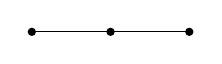
\begin{tikzpicture}
      \node [circ] {};
      \node [circ] at (2, 0) {};
      \node [circ] at (1, 0) {};
      \draw (0, 0) -- (2, 0);
    \end{tikzpicture}
  \end{center}
  We can degenerately describe this as first barycentrically subdividing the boundary (which does nothing in this case), and then add the barycenter.

  In the case of a $2$-simplex:
  \begin{center}
    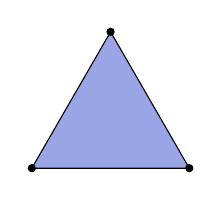
\begin{tikzpicture}
      \draw [fill=mblue, fill opacity=0.5] (0, 0) -- (2, 0) -- (1, 1.732) -- cycle;
      \node [circ] at (0, 0) {};
      \node [circ] at (2, 0) {};
      \node [circ] at (1, 1.732) {};
    \end{tikzpicture}
  \end{center}
  we first barycentrically subdivide the boundary:
  \begin{center}
    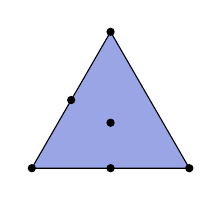
\begin{tikzpicture}
      \draw [fill=mblue, fill opacity=0.5] (0, 0) -- (2, 0) -- (1, 1.732) -- cycle;
      \node [circ] at (0, 0) {};
      \node [circ] at (2, 0) {};
      \node [circ] at (1, 1.732) {};
      \node [circ] at (1, 0) {};
      \node [circ] at (0.5, 0.866) {};
      \node [circ] at (1, 0.5773) {};
    \end{tikzpicture}
  \end{center}
  Then add the barycenter $b_x$, and for each standard simplex in the boundary, we ``cone it off'' towards $b_x$:
  \begin{center}
    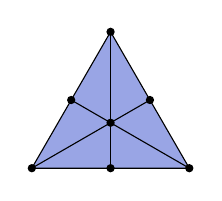
\begin{tikzpicture}
      \draw [fill=mblue, fill opacity=0.5] (0, 0) -- (2, 0) -- (1, 1.732) -- cycle;
      \node [circ] at (0, 0) {};
      \node [circ] at (2, 0) {};
      \node [circ] at (1, 1.732) {};
      \node [circ] at (1, 0) {};
      \node [circ] at (0.5, 0.866) {};
      \node [circ] at (1.5, 0.866) {};
      \node [circ] at (1, 0.5773) {};
      \draw (0, 0) -- (1, 0.5773) -- (2, 0);
      \draw (1, 0) -- (1, 1.732);
      \draw (0.5, 0.866) -- (1, 0.5773) -- (1.5, 0.866);
    \end{tikzpicture}
  \end{center}
  More formally, in the standard $n$-simplex $\Delta^n \subseteq \R^{n + 1}$, we let $B_n$ be its barycenter. For each singular $i$-simplex $\sigma: \Delta^i \to \Delta^n$, we define
  \[
    \mathrm{Cone}^{\Delta^n}_i (\sigma): \Delta^{i + 1} \to \Delta^n
  \]
  by
  \[
    (t_0, t_1, \cdots, t_{i + 1}) \mapsto t_0 b_n + (1 - t_0) \cdot \sigma\left(\frac{(t_1, \cdots, t_{i + 1})}{1 - t_0}\right).
  \]
  We can then extend linearly to get a map $\mathrm{Cone}_i^{\Delta^n}: C_i(\Delta^n) \to C_{i + 1}(\Delta^n)$.

  Since this increases the dimension, we might think this is a chain map. Then for $i > 0$, we have
  \begin{align*}
    d \mathrm{Cone}_i^{\Delta^n}(\sigma) &= \sum_{j = 0}^{i + 1} \mathrm{Cone}_i^{\Delta^n}(\sigma) \circ \delta_j \\
    &= \sigma + \sum_{j = 1}^{i + 1} (-1)^j \mathrm{Cone}_{i - 1}^{\Delta^n} (\sigma \circ \delta_{j - 1})\\
    &= \sigma - \mathrm{Cone}_{i - 1}^{\Delta^n} (d \sigma).
  \end{align*}
  For $i = 0$, we get
  \[
    d \mathrm{Cone}_i^{\Delta^n}(\sigma) = \sigma - \varepsilon(\sigma) \cdot b_n,
  \]
  In total, we have
  \[
    d \mathrm{Cone}_i^{\Delta^n} + \mathrm{Cone}_{i - 1}^{\Delta^n} d = \mathrm{id} - c_{\Cdot},
  \]
  where $c_i = 0$ for $i > 0$, and $c_0(\sigma) = \varepsilon(\sigma) b_n$ is a map $C_\Cdot(\Delta^n) \to C_\Cdot(\Delta^n)$.

  We now want to construct a barycentric subdivision map $\rho_n^X: C_n(X) \to C_n(X)$, and insist that it is natural that if $f: X \to Y$ is a map, then $f_\# \circ \rho_n^X = \rho_n^Y \circ f_\#$, ie. the diagram
  \[
    \begin{tikzcd}
      C_n(X) \ar[r, "\rho_n^X"] \ar[d, "f_\#"] & C_n(X) \ar[d, "f_\#"]\\
      C_n(Y) \ar[r, "\rho_n^Y"] & C_n(Y)
    \end{tikzcd}.
  \]
  So if $\sigma: \Delta^n \to X$, we let $\iota_n: \Delta^n \to \Delta^n \in C_n(\Delta^n)$ be the identity map. Then we must have
  \[
    \rho_n^X (\sigma) = \rho_n^X (\sigma_\# \iota_n) = \sigma_\# \rho_n^{\Delta^n}(\iota_n).
  \]
  So if know how to do barycentric subdivision for $\iota_n$ itself, then by naturality, we have defined it for all spaces! Naturality makes life easier for us, not harder!

  So we define $\rho_n^X$ recursively on $n$, for all spaces $X$ at once, by
  \begin{enumerate}
    \item $\rho_0^X = \id_{C_0}(X)$
    \item For $n > 0$, we define the barycentric subdivision of $\iota_n$ by
      \[
        \rho_n^{\Delta^n}(\iota_n) = \mathrm{Cone}_{n - 1}^{\Delta^n} (\rho_{n - 1}^{\Delta^n} (\d \iota_n)),
      \]
      and then extend by naturality.
  \end{enumerate}
\end{defi}

\begin{lemma}
  $\rho_\Cdot^X$ is a natural chain map.
\end{lemma}

\begin{lemma}
  $\rho_\Cdot^X$ is chain homotopic to the identity.
\end{lemma}

\begin{proof}
  No one cares.
\end{proof}

\begin{lemma}
  The diameter of each subdivided simplex in $(\rho_n^{\Delta^n})^k(\iota_n)$ is bounded by $\left(\frac{n}{n + 1}\right)^k \diam(\Delta^n)$.
\end{lemma}

\begin{proof}
  Basic geometry.
\end{proof}

\begin{prop}
  If $c \in C_n^\mathcal{U}(X)$, then $p^X(c) \in C_n^{\mathcal{U}}(X)$.

  Moreover, if $c \in C_n(X)$, then there is some $k$ such that $(\rho_n^{X})^k(c) \in C_n^{\mathcal{U}}(X)$.
\end{prop}

\begin{proof}
  The first part is clear. For the second part, note that every chain is a finite sum of simplices. So we only have to check it for single simplices. We let $\sigma$ be a simplex, and let
  \[
    \mathcal{V} = \{\sigma^{-1} \mathring{U}_\alpha\}
  \]
  be an open cover of $\Delta^n$. By the Lebesgue number lemma, there is some $\varepsilon > 0$ such that any set of diameter $< \varepsilon$ is contained in some $\sigma^{-1} \mathring{U}_\alpha$. So we can choose $k > 0$ such taht $(\rho_n^{\Delta^n}) (\iota_n)$ is a sum of simplices which each has diameter $< \varepsilon$. So each lies in some $\sigma^{-1}\mathring{U}_\alpha$. So
  \[
    (\rho_n^{\Delta^n})^k (\iota_n) = C_n^{\mathcal{V}} (\Delta^n).
  \]
  So applying $\sigma$ tells us
  \[
    (\rho_n^{\Delta^n})^k (\sigma) \in C_n^\mathcal{U}(X).
  \]
\end{proof}

Finally, we get to the theorem.
\begin{thm}[Small simplices theorem]\index{small simplices theorem}
  The natural map $U: H_*^\mathcal{U}(X) \to H_*(X)$ is an isomorphism.
\end{thm}

\begin{proof}
  Let $[c] \in H_n(X)$. By the proposition, there is some $k > 0$ such that $(\rho_n^X)^k (c) \in C_n^{\mathcal{U}}(x)$. We know that $\rho_n^X$ is chain homotopic to the identity. Thus so is $(\rho_n^X)^k$. So $[(\rho_n^X)^k (c)] = [c]$. So the map $H_n^\mathcal{U}(X) \to H_n(X)$ is surjective.

  To show that it is injective, we suppose $U([c]) = 0$. Then we can find some $z \in H_{n + 1}(X)$ such that $dz = c$. We can then similarly subdivide $z$ enough such that it lies in $C^\mathcal{U}_{n + 1}(X)$. So this shows that $[c] = 0 \in H_n^{\mathcal{U}}(X)$.
\end{proof}

\section{Cell complexes}
\begin{defi}[Cell complex]\index{cell complex}
  A \emph{cell complex} is a space obtained as follows:
  \begin{enumerate}
    \item $X^0$ is a discrete space. The set of points in $X^0$ are called $I_0$.
    \item If $X^{n - 1}$ has been constructed, then we may choose a family of maps $\{\varphi_\alpha: S^{n - 1} \to X^{n - 1}\}_{\alpha \in I_n}$, and set
      \[
        X^n = \left(X^{n - 1} \amalg \left(\coprod_{\alpha \in I_n} D_\alpha^n\right) \right)/\{x \in \partial D_\alpha^n \sim \varphi_\alpha(x) \in X^{n - 1}\}.
      \]
      We call $X^n$ the \term{$n$-skeleton} of $X$ We call the image of $D_\alpha^n \setminus \partial D_\alpha^n$ in $X^n$ the \term{open cell} $e_\alpha$.
    \item Finally, we define
      \[
        X = \bigcup_{n \geq 0} X^n
      \]
      with the \term{weak topology}, namely that $A \subseteq X$ is open if $A \cap X^n$ is open in $X^n$ for all $n$.
  \end{enumerate}
\end{defi}

\begin{defi}[Finite-dimensional cell complex]\index{finite-dimensional cell complex}\index{cell complex!finite-dimensional}
  If $X = X^n$ for some $n$, we say $X$ is \emph{finite-dimensional}.
\end{defi}

\begin{defi}[Finite cell complex]\index{finite cell complex}\index{cell complex!finite}
  If $X$ is finite-dimensional and $I_n$ are all finite, then we say $X$ is \emph{finite}.
\end{defi}

We write $\Phi_\alpha: D_\alpha^n \to X^n$ for the obvious map. This is called the \term{characteristic map} for the cell $e_\alpha$.
\begin{defi}[Subcomplex]\index{subcomplex}\index{cell complex!subcomplex}
  A subcomplex $A$ of $X$ is a simplex obtained by using a subset $I_n' \subseteq I_n$.
\end{defi}
Note that we cannot simply throw away some cells to get a subcomplex, as the higher cells might want to map into the cells you have thrown away, and you need to remove them as well.

We have the following fact:
\begin{lemma}
  If $A \subseteq X$ is a subcomplex, then the pair $(X, A)$ is \emph{good}.
\end{lemma}

\begin{proof}
  See Hatcher 0.16.
\end{proof}

\begin{cor}
  If $A \subseteq X$ is a subcomplex, then
  \[
    \begin{tikzcd}
      H_n(X, A) \ar[r, "\sim"] & \tilde{H}_n(X/A)
    \end{tikzcd}
  \]
  is an isomorphism.
\end{cor}

\begin{lemma}
  Let $X$ be a cell complex. Then
  \begin{enumerate}
    \item
      \[
        H_i(X^n, X^{n - 1}) =
        \begin{cases}
          0 & i \not= n\\
          \bigoplus_{i \in I_n} \Z & i = n
        \end{cases}.
      \]
    \item $H_i(X^n) = 0$ for all $i > n$.
    \item $H_i(X^n) \to H_i(X)$ is an isomorphism for $i < n$.
  \end{enumerate}
\end{lemma}

\begin{proof}\leavevmode
  \begin{enumerate}
    \item As $(X^n, X^{n - 1})$ is good, we have an isomorphism
      \[
        \begin{tikzcd}
          H_i(X^n, X^{n - 1}) \ar[r, "\sim"] & \tilde{H}_i(X^n/X^{n - 1})
        \end{tikzcd}.
      \]
      But we have
      \[
        X^n/X^{n - 1} \cong \bigvee_{\alpha \in I_n} S_\alpha^n,
      \]
      the space obtained from $Y = \coprod_{\alpha \in I_n}S_\alpha^n$ by collapsing down the subspace $Z = \{x_\alpha: \alpha \in I_n\}$, where each $x_\alpha$ is the south pole of the sphere. We then note that $(Z, Y)$ is good, and so we have a long exact sequence
      \[
        \begin{tikzcd}
          H_i(Z) \ar[r] & H_i(Y) \ar[r] & \tilde{H}_i(Y/Z) \ar[r] & H_{i - 1}(Z) \ar[r] & H_{i - 1}(Y)
        \end{tikzcd}
      \]
      By checking the different possible cases, we obtain the desired result.
    \item This follows by induction on $n$. We have a long exact sequence
      \[
        \begin{tikzcd}
          H_i(X^{n - 1}) \ar[r] & H_i(X^n) \ar[r] & H_i(X^n, X^{n - 1})
        \end{tikzcd}
      \]
      We know the first term vanishes, and the third term vanishes for $i > n$. So it follows that $H_i(X^n)$ vanishes.
    \item To avoid doing too much point-set topology, we suppose $X$ is finite-dimensional, so $X = X^m$ for some $m$. Then we have a long exact sequence
      \[
        \begin{tikzcd}
          H_{i + 1} (X^{n + 1}, X^n) \ar[r] & H_i(X^n) \ar[r] & H_i(X^{n + 1}) \ar[r] & H_i(X^{n + 1}, X^n)
        \end{tikzcd}
      \]
      Now if $i < n$, we know the first and last groups vanish. So we have $H_i(X^n) \cong H_i(X^{n + 1})$. By continuing, we know that
      \[
        H_i(X^n) \cong H_i(X^{n + 1}) \cong H_i(X^{n + 2}) \cong \cdots \cong H_i(X^m) = H_i(X).
      \]
      To prove this for the general case, we need to use the fact that any map from a compact space to a cell complex hits only finitely many cells, and then the result would follow from this special case.
  \end{enumerate}
\end{proof}

For a cell complex $X$, let
\[
  C_n^{\mathrm{cell}}(X) = H_n(X^n, X^{n - 1}) \cong \bigoplus_{\alpha \in I_n} \Z.
\]
We define $d_n^{\mathrm{cell}}: C_n^{\mathrm{cell}}(X) \to C_{n - 1}^{\mathrm{cell}}(X)$ by the composition
\[
  \begin{tikzcd}
    H_n(X^n, X^{n - 1}) \ar[r, "\partial"] & H_n(X^{n - 1}) \ar[r, "q"] & H_{n - 1}(X^{n - 1}, X^{n - 2})
  \end{tikzcd}.
\]
We consider
\[
  \begin{tikzcd}[row sep=large, column sep=-0.5em]
    &&& 0\\
    0 \ar[dr] && H_n(X^{n + 1}) \ar[ur]\\
    &H_n(X^n) \ar[ur] \ar[dr, "q_n"]\\
    H_{n + 1}(X^{n + 1}, X^n) \ar[ur, "\partial"] \ar[rr, "d_{n + 1}^{\mathrm{cell}}"] & & H_n(X^n, X^{n - 1}) \ar[rr, "d_n^{\mathrm{cell}}"] \ar[rd, "\partial"] && H_{n - 1}(X^{n - 1}, X^{n - 2})\\
    & & & H_{n - 1}(X^{n - 1}) \ar[rd] \ar[ru, "q_{n - 1}"]\\
    & & 0 \ar[ur] & & H_{n - 1}(X^n)
  \end{tikzcd}
\]
Referring to the above diagram, we see that
\[
  d_n^{\mathrm{cell}} \circ d_{n + 1}^{\mathrm{cell}} = q_{n - 1} \circ \partial \circ q_n \circ \partial = 0,
\]
since the middle $\partial \circ q_n$ is part of an exact sequence. So $(C_{\Cdot}^{\mathrm{cell}}(X), d_{\Cdot}^{\mathrm{cell}})$ is a chain complex, and the corresponding homology groups are known as the \term{cellular homology} of $X$.

\begin{thm}
  \[
    H_n^{\mathrm{cell}}(X) \cong H_n(X).
  \]
\end{thm}

\begin{proof}
  We have
  \begin{align*}
    H_n(X) &\cong H_n(X^{n + 1}) \\
    &= H_n(X^n)/\im(\partial: H_{n + 1}(X^{n + 1}, X^n) \to H_n(X^n))\\
    \intertext{Since $q_n$ is injective, we have}
    &= q_n(H_n(X^n)) / \im(d_{n + 1}^{\mathrm{cell}}: H_{n + 1}(X^{n + 1}, X^n) \to H_n(X^n, X^{n - 1}))\\
    \intertext{By exactness, the image of $q_n$ is the kernel of $\partial$. So we have}
    &= \ker(\partial: H_n(X^n, X^{n - 1}) \to H_{n - 1}(X^{n - 1})) / \im(d_{n + 1}^{\mathrm{cell}})\\
    &= \ker(d_n^{\mathrm{cell}}) / \im(d_{n + 1}^{\mathrm{cell}})\\
    &= H_n^{\mathrm{cell}}(X).
  \end{align*}
\end{proof}

\begin{prop}
  If $X$ is a finite cell complex, then $H_n(X)$ is a finitely-generated abelian group for all $n$, generated by at most $|I_n|$ elements. In particular, if there are no $n$-cells, then $H_n(X)$ vanishes.

  If $X$ has a cell-structure with cells in even-dimensional cells only, then $H_*(X)$ are all free.
\end{prop}

We can similarly define cellular cohomology.
\begin{defi}[Cellular cohomology]\index{cellular cohomology}
  We define \emph{cellular cohomology} by
  \[
    C_{\mathrm{cell}}^n(X) = H^n(X^, X^{n - 1})
  \]
  and let $d_{\mathrm{cell}}^n$ be the composition
  \[
    \begin{tikzcd}
      H^n(X^n, X^{n - 1}) \ar[r, "q^*"] & H^n(X^n) \ar[r, "\partial"] & H^{n + 1}(X^{n + 1}, X^n).
    \end{tikzcd}
  \]
  This defines a cochain complex $C_{\mathrm{cell}}^\Cdot(X)$ with cohomology $H^*_{\mathrm{cell}}(X)$, and we have
  \[
    H_{\mathrm{cell}}^*(X) \cong H^*(X).
  \]
  One can directly check that
  \[
    C_{\mathrm{cell}}^\Cdot(X) \cong \Hom (C_\Cdot^{\mathrm{cell}}(X), \Z).
  \]
\end{defi}

To use cellular cohomology to calculate, we need to understand what the map
\[
  d_n^{\mathrm{cell}} : C_n^\Cdot(X) = \bigoplus_{\alpha \in I_n} \Z\{e_\alpha\} \to C_{n + 1}^{\mathrm{cell}} = \bigoplus_{\beta \in I_{n - 1}}\Z\{e_\beta\}
\]
is. In particular, we want to find the coefficients $d_{\alpha\beta}$ such that
\[
  d_n^{\mathrm{cell}}(e_\alpha) = \sum d_{\alpha\beta} e_\beta.
\]
It turn out this is pretty easy
\begin{lemma}
  The coefficients $d_{\alpha\beta}$ are given by the degree of
  \[
    \begin{tikzcd}
      S_\alpha^{n - 1} = \partial D_\alpha^n \ar[r, "\varphi_\alpha"] & X^{n - 1} \ar[r] & X^{n - 1}/X^{n - 2} = \bigwedge_{\gamma \in I_{n - 1}} S_\gamma^{n - 1} \ar[r] & S_\beta^{n - 1}
    \end{tikzcd},
  \]
  where the final map is obtained by collapsing the other spheres in the wedge.

  In the case of cohomology, the maps are given by the transposes of these.
\end{lemma}
This is easier in practice that in sounds. In practice, the map is given by ``the obvious one''.

\begin{proof}
  Consider the diagram
  \[
    \begin{tikzcd}
      H_n(D_\alpha^n, \partial D_\alpha^n) \ar[d, "(\Phi_\alpha)_*"] \ar[r, "\partial", "\sim"'] & H_{n - 1}(\partial D_\alpha^n)\ar[d, "(\varphi_\alpha)_*"] \ar[r, dashed] & \tilde{H}_{n - 1}(S^{n - 1}, \beta) \\
      H_n(X^n, X^{n - 1}) \ar[r, "\partial"] \ar[rd, "d_n^\mathrm{cell}"] & H_{n - 1}(X^{n - 1}) \ar[d, "q"] & \tilde{H}_{n - 1}\left(\bigwedge S_\gamma^{n - 1}\right)\ar[u, "\text{collapse}"]\\
      & H_{n - 1}(X^{n - 1}, X^{n - 2}) \ar[r, "\text{excision}", "\sim"'] & \tilde{H}_{n - 1}(X^{n - 1}/X^{n - 2})" \ar[u, equals]
    \end{tikzcd}
  \]
  By the long exact sequence, the top horizontal map is an isomorphism.

  Now let's try to trace through the diagram. We can find
  \[
    \begin{tikzcd}
      1 \ar[d, maps to] \ar[r, "\text{isomorphism}"] & 1 \ar[r, maps to, "\text{map in lemma}"]& d_{\alpha\beta}\\
      e_\alpha \ar[rd, maps to]\\
      & \sum d_{\alpha\gamma}e_\gamma \ar[r, maps to] & \sum d_{\alpha\gamma} e_\gamma \ar[uu, maps to]
    \end{tikzcd}
  \]
\end{proof}

\begin{eg}
  Let $K$ be the Klein bottle.
  \begin{center}
    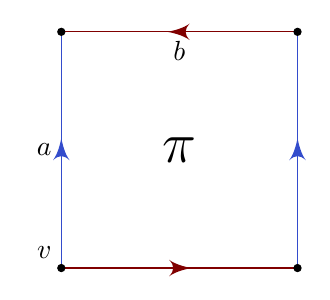
\begin{tikzpicture}
      \draw [->-=0.55, mred] (0, 0) -- (3, 0);
      \draw [->-=0.55, mred] (3, 3) -- (0, 3);
      \draw [->-=0.55, mblue] (3, 0) -- (3, 3);
      \draw [->-=0.55, mblue] (0, 0) -- (0, 3);

      \node [circ] at (0, 0) {};
      \node [circ] at (3, 0) {};
      \node [circ] at (0, 3) {};
      \node [circ] at (3, 3) {};
      \node [anchor = south east] {$v$};

      \node [left] at (0, 1.5) {$a$};
      \node [below] at (1.5, 3) {$b$};
      \node at (1.5, 1.5) {\huge $\pi$};
    \end{tikzpicture}
  \end{center}
  We give it a cell complex structure by
  \begin{itemize}
    \item $K^0 = \{v\}$. Note that all four vertices in the diagram are identified.
      \begin{center}
        \begin{tikzpicture}
          \node [circ] at (0, 0) {};
          \node [above] at (0, 0) {$v$};
        \end{tikzpicture}
      \end{center}
    \item $K^1 = \{a, b\}$.
      \begin{center}
        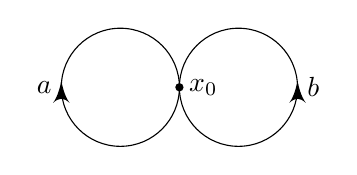
\begin{tikzpicture}[scale=0.75]
          \draw (-1, 0) circle [radius=1];
          \draw (1, 0) circle [radius=1];
          \node [circ] {};
          \node [left] at (-2, 0) {$a$};
          \node [right] at (2, 0) {$b$};
          \draw [->] (2, 0.1) -- (2, 0.11);
          \draw [->] (-2, 0.1) -- (-2, 0.11);
          \node [right] {$x_0$};
        \end{tikzpicture}
      \end{center}
    \item $K^2$ is the unique $2$-cell $\pi$ we see in the picture, where $\varphi_\pi: S^1 \to K^1$ given by $a b a^{-1}b$.
  \end{itemize}
  The cellular chain compmlex is given by
  \[
    \begin{tikzcd}[row sep=small]
      0 \ar[r] & C_2^{\mathrm{cell}}(K) \ar[d, equals] \ar[r, "d_2^{\mathrm{cell}}"] & C_1^{\mathrm{cell}}(K) \ar[d, equals] \ar[r, "d_1^{\mathrm{cell}}"] & C_0^{\mathrm{cell}}(K) \ar[d, equals]\\
      & \Z\pi & \Z a \oplus \Z b & \Z_v
    \end{tikzcd}
  \]
  We can now compute the maps $d_i^{\mathrm{cell}}$. The $d_1$ map is easy. We have
  \[
    d_1(a) = d_1(b) = v - v = 0.
  \]
  In the $d_2$ map, we can figure it out by using local degrees. If we think hard enough, we realize that if we collapse the $b$ loop, then the attaching map from $S^1$ ot $a$ is nullhomotopic, while the map to $b$ has degree $2$. So we have
  \[
    d_2(\pi) = 0a + 2b.
  \]
  So we have
  \begin{align*}
    H_0(K) &= \Z\\
    H_1(K) &= \frac{\Z \oplus \Z}{\bra2b\ket} = \Z \oplus \Z/2\Z\\
    H_2(K) &= 0
  \end{align*}
  We can similarly compute the cohomology. By dualizing, we have
  \[
    \begin{tikzcd}[row sep=small]
      C_{\mathrm{cell}}^2(K)(K) \ar[d, equals] & C_{\mathrm{cell}}^1(K) \ar[d, equals] \ar[l, "(0\; 2)"] & C_{\mathrm{cell}}^0(K) \ar[d, equals] \ar[l, "(0)"] \\
      \Z & \Z \oplus \Z & \Z
    \end{tikzcd}
  \]
  So we have
  \begin{align*}
    H_0(K) &= \Z\\
    H_1(K) &= \Z\\
    H_2(K) &= \Z/2\Z
  \end{align*}
  Note that the second cohomology is \emph{not} the dual of the second homology!

  However, if we forget where each factor is, and just add all the homology groups together, we get $\Z \oplus \Z \oplus \Z/2\Z$. Also, if we forget all the torsion components $\Z/2\Z$, then they are the same!

  This is a general phenomenon. For a cell complex, if we know what all the homology groups are, we can find the cohomologies by keeping the $\Z$'s unchanged and moving the torsion components up. The general statement will be given by the \emph{univeresal coefficient theorem}.
\end{eg}

\begin{eg}
  Consider $\RP^n = S^n/(x \sim -x)$. We notice that for any point in $\RP^n$, if it is not in the equator, then it is represented by a unique element in the norther hemisphere. Otherwise, it is represented by two points. So we have $\RP^n \cong D^n/(x \sim -x\text{ for }x \in \partial D^n)$. This is a nice description, since if we throw out the interior of the disk, then we are left with an $S^{n - 1}$ with antipodal points identified, ie. an $\RP^{n - 1}$! So we can immediately see that
  \[
    \RP^n = \RP^{n - 1} \cup_f D^n,
  \]
  for $f: S^{n - 1} \to \RP^{n - 1}$ given by
  \[
    f(x) = [x].
  \]
  So $\RP^n$ has a cell structure with one cell in every degree up to $n$. What are the boundary maps?

  We write $e_i$ for the $i$-th degree cell. We know that $e_i$ is attached along the map $f$ described above. More concretely, we have
  \[
    \begin{tikzcd}
      f: S_s^{i - 1}\ar[r, "\varphi_i"] & \RP^{i - 1} \ar[r] &\RP^{i - 1}/\RP^{i - 2} = S_t^{i - 1}
    \end{tikzcd}.
  \]
  The open upper hemisphere and lower hemisphere of $S^{i - 1}_s$ are mapped homeomorphically to $S_t^{i - 1} \setminus \{*\}$. Furthermore,
  \[
    f|_{\mathrm{upper}} = f|_{\mathrm{lower}} \circ a,
  \]
  where $a$ is the antipodal map. But we know that $\deg(a) = (-1)^i$. So we have a zero map if $i$ is odd, and a $2$ map if $i$ is even. Then we have
  \[
    \begin{tikzcd}
      \cdots \ar[r, "2"] & \Z e_3 \ar[r, "0"] & \Z e_2 \ar[r, "2"] & \Z e_1 \ar[r, "0"] & \Z e_0
    \end{tikzcd}.
  \]
  What happens on the left end depends on whether $n$ is even or odd. So we have
  \[
    H_i(\RP^n) =
    \begin{cases}
      \Z & i = 0\\
      \Z/2\Z & i\text{ odd}, i < n\\
      0 & i\text{ even}, 0 < i < n\\
      \Z & i = n\text{ is odd}\\
      0 & \text{otherwise}
    \end{cases}.
  \]
  We can immediately work out the cohomology too. We will just write out the answer:
  \[
    H^i(\RP^n) =
    \begin{cases}
      \Z & i = 0\\
      0 & i\text{ odd}, i < n\\
      \Z/2\Z & i\text{ even}, 0 < i \leq n\\
      \Z & i = n\text{ is odd}\\
      0 & \text{otherwise}
    \end{cases}.
  \]
\end{eg}

\section{(Co)homology with coefficients}
Recall that when we defined (co)homology, we constructed these free $\Z$-modules from our spaces. However, we did not actually use the fact that it was $\Z$, we might as well replace it with any abelian group $A$.

\begin{defi}[(Co)homology with coefficients]\index{homology!with coefficients}\index{cohomology!with coefficients}
  Let $A$ be an abelian group, and $X$ be a topological space. We let
  \[
    C_{\Cdot}(X, A) = C_\Cdot(X) \otimes A
  \]
  with differentials $d \otimes \id_A$. We let
  \[
    H_n(X; A) = H_n(C_{\Cdot}(X, A), d \otimes \id_A).
  \]
  We can also define
  \[
    H_n^{\mathrm{cell}}(X, A) = H_n(C_{\Cdot}^{\mathrm{cell}}(X) \otimes A),
  \]
  and the same proof shows that $H_n^{\mathrm{cell}}(X; A) = H_n(X; A)$.

  Similarly, we let
  \[
    C^{\Cdot}(X; A) = \Hom(C_{\Cdot}(X), A),
  \]
  with the usual (dual) differential. We again set
  \[
    H^n(X; A) = H^n(C^\Cdot(X; A)).
  \]
  We similarly define cellular cohomology.
\end{defi}
We will usually take $A = \Z, \Z/n\Z$ or $\Q$.

\begin{eg}
  In the case of $C_{\Cdot}^{\mathrm{cell}}(\RP^n)$, the differentials are all $0$ or $2$. So in $C_\Cdot^{\mathrm{cell}}(\RP^n, \Z/2)$, all the differentials are $0$. So we have
  \[
    H_i(\RP^n, \Z/2) =
    \begin{cases}
      \Z/2 & 0 \leq i \leq n\\
      0 & i > n
    \end{cases}
  \]
  Similarly, the cohomology groups are the same.

  On the other hand, if we take the coefficients to be $\Q$, then multiplication by $2$ is now an isomorphism. Then we get
  \[
    C_{\Cdot}^\mathrm{cell}(\RP^n, \Q)
    \begin{cases}
      \Q & n \text{ odd}\\
      0 & n\text{ even}
    \end{cases}
  \]
  for $n$ not too large.
\end{eg}

\subsection{Euler characteristic}
There are many ways to define the Euler characteristic, and they are all equivalent. So to define it, we pick a definition that makes it obvious it is a number.
\begin{defi}[Euler characteristic]\index{Euler characteristic}
  Let $X$ be a cell complex. We let
  \[
    \chi(X) = \sum_n (-1)^n \text{number of $n$-cells of $X$} \in \Z.
  \]
\end{defi}
From this definition, it is not clear that this is a property of $X$ itself, rather than something about its cell decomposition.

We similarly define
\[
  \chi_{\Z}(X) = \sum_n (-1)^n \rank H_n(X; \Z).
\]
For any field $\F$, we define
\[
  \chi_{\F}(X) = \sum_n (-1)^n \dim_\F H_n(X; \F).
\]
\begin{thm}
  We have
  \[
    \chi = \chi_\Z = \chi_\F.
  \]
\end{thm}

\begin{proof}
  First note that the number of $n$ cells of $X$ is the rank of $C_n^{\mathrm{cell}}(X)$, which we will just write as $C_n$. Let
  \begin{align*}
    Z_n &= \ker (d_n: C_n \to C_{n - 1})\\
    B_n &= \im (d_{n + 1}: C_{n + 1} \to C_n).
  \end{align*}
  We are now going to write down two short exact sequences. By definition of homology, we have
  \[
    \begin{tikzcd}
      0 \ar[r] & B_n \ar[r] & Z_n \ar[r] & H_n(X; \Z) \ar[r] & 0
    \end{tikzcd}.
  \]
  Also, the definition of $Z_n$ and $B_n$ give us
  \[
    \begin{tikzcd}
      0 \ar[r] & Z_n \ar[r] C_n \ar[r] & B_{n - 1} \ar[r] & 0
    \end{tikzcd}.
  \]
  We will now use the first isomorphism theorem to know that the rank of the middle term is the sum of ranks of the outer terms. So we have
  \[
    \chi_\Z(X) = \sum (-1)^n \rank H_n(X) = \sum(-1)^n (\rank Z_n - \rank B_n).
  \]
  We also have
  \[
    \rank B_n = \rank C_{n + 1} - \rank Z_{n + 1}.
  \]
  So we have
  \begin{align*}
    \chi_\Z(X) &= \sum_n (-1)^n (\rank Z_n - \rank C_{n + 1} + \rank Z_{n + 1}) \\
    &= \sum_n (-1)^{n + 1} \rank C_{n + 1} \chi(X).
  \end{align*}
  For $\chi_\F$, we use the fact that
  \[
    \rank C_n = \dim_{\F} C_n \otimes \F.
  \]
\end{proof}
\section{Cup product}
So far, homology and cohomology are somewhat similar. We computed them, saw they are not the same, but they seem to contain the same information nevertheless. However, cohomology is 10 times better, because we can define a ring structure on them, and rings are better than groups.

Just like the case of homology and cohomology, we will be able to write down the definition easily, but will struggle to compute it.

\begin{defi}[Cup product]\index{cup product}\index{$\smile$}
  Let $R$ be a commutative ring, and $\phi \in C^k(X, R)$, $\psi \in C^\ell(X, R)$. Then $\phi \smile \psi \in C^{k + \ell}(X; R)$ is given by
  \[
    (\phi \smile \psi)(\sigma: \Delta^{k + \ell} \to X) = \phi(\sigma|_{[v_1, \ldots, v_k]}) \cdot \psi(\sigma|_{[v_k, \ldots, v_{k + \ell}]}).
  \]
  Here the multiplication is multiplication in $R$, and $v_0, \cdots, v_\ell$ are the vertices of $\Delta^{k + \ell} \subseteq \R^{k + \ell + 1}$, and the restriction is given by
  \[
    \sigma|_{[x_0, \ldots, x_i]} (t_0, \ldots, t_i) = \sigma\left(\sum t_j x_j\right).
  \]
  This is a bilinear map.
\end{defi}

\begin{notation}
  We write
  \[
    H^*(X; R) = \bigoplus_{n \geq 0} H^n(X, R).
  \]
\end{notation}
This is the definition. We can try to establish some of its basic properties. We want to know how this interacts with the differential $d$ with the cochains. The obvious answer $d(\phi \smile \psi) = (\d \phi) \smile (\d \psi)$ doesn't work, because the degrees are wrong. What we have is:

\begin{lemma}
  If $\phi \in C^k(X; R)$ and $\psi \in C^\ell(X, R)$, then
  \[
    d (\phi \smile \psi) = (d \phi)\smile \psi + (-1)^k \phi\smile(d \psi).
  \]
\end{lemma}

\begin{proof}
  Let $\sigma: \Delta^{k + \ell + 1} \to X$ be a simplex. Then we have
  \begin{align*}
    ((\d \phi)\smile \psi)(\sigma) &= (\d \phi)(\sigma|_{[v_0, \ldots, v_{k + 1}]}) \cdot \psi(\sigma|_{[v_{k + 1}, \ldots, v_{k + \ell + 1}]})\\
    &= \phi\left(\sum_{i = 0}^{n + 1} (-1)^i \sigma|_{[v_0, \ldots, \hat{v}_i, \ldots, v_{k + 1}]}\right) \cdot \psi(\sigma|_{[v_{k + 1}, \ldots, v_{k + \ell + 1}]})\\
    (\phi \smile (\d \psi))(\sigma) &= \phi(\sigma|_{[v_0, \ldots, v_k]}) \cdot (\d \psi)(\sigma|_{v_k,\ldots, v_{k + \ell + 1}]})\\
    &=\phi(\sigma|_{[v_0, \ldots, v_k]}) \cdot \psi\left(\sum_{i = k}^{k + \ell + 1} (-1)^{i - k} \sigma|_{[v_k, \ldots, \hat{v}_i, \ldots, v_{k + \ell + 1}]}\right)\\
    &=(-1)^k \phi(\sigma|_{[v_0, \ldots, v_k]}) \cdot \psi\left(\sum_{i = k}^{k + \ell + 1} (-1)^{i} \sigma|_{[v_k, \ldots, \hat{v}_i, \ldots, v_{k + \ell + 1}]}\right).
  \end{align*}
  We notice that the last term of the first expression, and the first term of the second expression are exactly the same, except the signs differ by $-1$. Then the remaining terms overlap in exactly 1 vertex, so the expression is equal to
  \[
    (\phi \smile \psi)(\d \sigma) = (\d (\phi \smile \psi))(\sigma)
  \]
  as required.
\end{proof}
This is the most interesting thing about these things, because it tells us this gives a well-defined map on cohomology.

\begin{cor}
  The cup product induces a well-defined map
  \[
    \begin{tikzcd}[row sep = 0ex
        ,/tikz/column 1/.append style={anchor=base east}
        ,/tikz/column 2/.append style={anchor=base west}
      ]
      \smile: H^k(X; R) \times H^k(X; R) \ar[r] & H^{k + \ell}(X; R)\\
      ([\phi], [\psi] ) \ar[r, maps to] & \lbrack\phi \cup \psi\rbrack
    \end{tikzcd}
  \]
\end{cor}

\begin{proof}
  To see this is defined at all, as $\d \phi = 0 = \d \psi$, we have
  \[
    \d (\phi \smile \psi) = (\d \phi) \smile \psi \pm \phi \smile (\d \psi) = 0.
  \]
  So $\phi \smile \psi$ is a cocycle, and represents the cohomology class. To see this is well-defined

  If $\phi' = \phi + \d\tau$, then
  \[
    \phi' \smile \psi = \phi \smile \psi + d \tau \smile \psi = \phi \smile \psi + d(\tau \smile \psi) \pm \tau \smile (\d \psi).
  \]
  Using the fact that $\d \psi = 0$, we know that $\phi' \smile \psi$ and $\phi \smile \psi$ differ by a boundary, so $[\phi' \smile \psi] = [\phi \smile \psi]$. The case where we change $\psi$ is similar.
\end{proof}

Note that the operation $\smile$ is associative on cochains, so associative on $H^*$ too.

Also, there is a map $1: C_0(X) \to R$ sending $\sigma \mapsto 1$ for all $\sigma$. Then we have
\[
  [1] \smile [\phi] = [\phi].
\]
So we have
\begin{prop}
  $(H^*(X; R), \smile, [1])$ is a unital ring.
\end{prop}
Note that this is not commutative!

Moreover, we have
\begin{prop}
  If $f: X \to Y$ is a cup product, and $x, y \in H^*(Y; R)$, then
  \[
    f^*(a \smile b) = f^*(a) \smile f^*(b).
  \]
  So $f^*$ is a homomorphism of unital rings.
\end{prop}

\begin{defi}[Cross product]\index{cross product}
  If we let $\pi_X: X \times Y \to X$, $\pi_Y: X \times Y\to Y$ be the projection maps, then we have a \emph{cross product}
  \[
    \begin{tikzcd}[row sep = 0ex
        ,/tikz/column 1/.append style={anchor=base east}
        ,/tikz/column 2/.append style={anchor=base west}
      ]
      \times: H^k(X; R) \otimes_R H^\ell(Y; R) \ar[r] & H^{k + \ell}(X \times Y; R)\\
      a \otimes b \ar[r, maps to] & (\pi_X^* a) \smile (\pi_Y^* b)
    \end{tikzcd}.
  \]
\end{defi}
Note that the diagonal map $\Delta: X \to X \times X$ given by $\Delta(x) = (x, x)$ satisfies.
\[
  \Delta^*(a \times b) = a \smile b
\]
for all $a, b \in H^*(X; R)$. So these two products determine each other.

\begin{prop}
  Let $R$ be a commutative ring. If $\alpha \in H^k(X, R)$ and $\beta \in H^\ell(X, R)$, then we have
  \[
    \alpha \smile \beta = (-1)^{k\ell}\beta \smile \alpha
  \]
\end{prop}
We say $R$ is \term{graded commutative}.

Note that this is only true for the cohomology classes. It is not true in general for the cochains. So we would expect that this is rather annoying to prove.

\begin{proof}
  Let $\rho_n: C_n(X) \to C_n(x)$ be given by
  \[
    \sigma \mapsto (-1)^{n(n + 1)/2} \sigma|_{[v_n, v_{n - 1}, \ldots, v_0]}
  \]
  The $\sigma|_{[v_n, v_{n - 1}, \ldots, v_0]}$ tells us that we reverse the order of the vertices, and the factor of $(-1)^{n(n + 1)/2}$ is the sign of the permutation that reverses $0, \cdots, n$. For convenience, we write
  \[
    \varepsilon_n = (-1)^{n (n + 1)/2}.
  \]
  \begin{claim}
    We claim that $\rho_{\Cdot}$ is a chain map, and is chain homotopic to the identity.
  \end{claim}
  Suppose the claim holds. We let $\phi \in C^k(X, R)$ represent $\alpha$ and $\psi \in C^\ell(X, R)$ represent $\beta$. Then we have
  \begin{align*}
    (\rho^* \phi \smile \rho^* \psi)(\sigma) &= (\rho^* \phi)(\sigma|_{[v_0, \ldots, v_k]} (\rho^* \psi)(\sigma|_{[v_k, \ldots, v_{k + \ell}]})\\
    &= \phi(\varepsilon_k \cdot \sigma|_{[v_k, \ldots, v_0]}) \psi(\varepsilon_\ell \sigma|_{[v_{k + \ell}, \ldots, v_k]}).
  \end{align*}
  Similarly, we can compute
  \begin{align*}
    \rho^*(\psi \smile \phi)(\sigma) &= (\psi \smile \phi)(\varepsilon_{k + \ell} \sigma|_{[v_{k + \ell}, \ldots, v_0]}\\
    &= \varepsilon_{k + \ell} \psi(\sigma|_{[v_{k + \ell}, \ldots, v_k}]) \phi(\sigma|_{[v_k, \ldots, v_0]})\\
    &= \varepsilon_{k + \ell}\varepsilon_k \varepsilon_\ell (\rho^* \phi) \smile (\rho^* \psi)(\sigma).
  \end{align*}
  By checking it directly, we can see that $\varepsilon_{n + \ell}\varepsilon_k \varepsilon_\ell = (-1)^{k\ell}$. So we have
  \begin{align*}
    \alpha \smile \beta &= [\phi \smile \psi] \\
    &= [\rho^* \phi \smile \rho^* \psi] \\
    &= (-1)^{k\ell}[\rho^*(\psi \smile \phi)] \\
    &= (-1)^{k\ell}[\psi \smile \phi] \\
    &= (-1)^{kl} \beta \smile \alpha.
  \end{align*}
  Now it remains to prove the claim. We have
  \begin{align*}
    \d \rho(\sigma) &= \varepsilon_n \sum_{i = 0}^n (-1)^j \sigma|_{[v_n, \ldots, \hat{v}_{n - i}, \ldots, v_0]}\\
    \rho(\d \sigma) &= \rho(\sum_{i = 0}^n (-1)^i \sigma|_{[v_0, \ldots, \hat{v}_i, \ldots., v_n]}\\
    &= \varepsilon_{n - 1} \sum_{j = 0}^n (-1)^j \sigma|_{[v_n, \ldots, \hat{v}_j, v_0]}.
  \end{align*}
  We now notice that $\varepsilon_{n - 1}(-1)^{n - i} = \varepsilon_n (-1)^i$. So this is a chain map!

  We now define a chain map. We let
  \[
    P_n = \sum_i (-1)^i \varepsilon_{n - i} [v_0, \cdots, v_i, w_n, \cdots, w_i] \in C_{n + 1}([0, 1] \times \Delta^n),
  \]
  where $v_0, \cdots, v_n$ are the vertices of $\{0\} \times \Delta^n$ and $w_0, \cdots, w_n$ are the vertices of $\{1\} \times \Delta^n$.

  We let $\pi: [0, 1] \times \Delta^n \to \Delta^n$ be the projection, and let $F_n^X: C_n(X) \to C_{n + 1}(X)$ be given by
  \[
    \sigma \mapsto (\sigma \circ \pi)_\#(P_n).
  \]
  We calculate
  \begin{align*}
    \d F_n^X(\sigma) &= (\sigma \circ \pi)_\#(\d P_n) \\
    &= (\sigma \circ \pi_\#)\left(\sum_i \left(\sum_{j \leq i}(-1)^j (-1)^i \varepsilon_{n - i}[v_0, \cdots, \hat{v}_j, \cdots, v_i, w_0, \cdots, w_i]\right)\right.\\
    &\quad +\left.\left(\sum_{j \geq i} (-1)^{n + i + 1 - j}(-1)^i \varepsilon_{n - i}[v_0, \cdots, v_i, w_n, \cdots, \hat{w}_j, \cdots, v_i]\right)\right).
  \end{align*}
  The terms with $j = i$ give
  \begin{align*}
    &(\sigma \circ \pi)_\#\left(\sum_i \varepsilon_{n - i}[v_0, \cdots, v_{i - 1}, w_n, \cdots, w_i]\right. \\
    &\quad+ \left.\sum_i (-1)^{n + 1}(-1)^i \varepsilon_{n - i}[v_0, \cdots, v_i, w_n,\cdots, w_{i + 1}]\right)\\
    ={}& (\sigma \circ \pi)_\#(\varepsilon_n[w_n,\cdots, w_0] - [v_0, \cdots, v_n])\\
    ={}& \rho(\sigma) - \sigma
  \end{align*}
  The terms with $j \not= i$ are precisely $-F_{n - 1}^\times (\d \sigma)$ as required. It is easy to see that the terms are indeed the right terms, and we just have to check that the signs are right. I'm not doing that.
\end{proof}
There is also a \emph{relative cup} product
\[
  \smile: H^k(X, A; R) \otimes H^k(X, R) \to H^{k + \ell}(X, A; R)
\]
given by the same formula. Indeed, to see this is properly defined, note that if $\phi \in C^k(X, A; R)$, then $\phi$ is a map
\[
  \phi:C_k(X, A) = \frac{C-k(X)}{C_k(A)} \to R.
\]
In other words, it is a map $C_K(X) \to R$ that vanishes on $C_k(A)$. Then if $\sigma \in C_{n + \ell}(A)$ and $\psi \in C^\ell(X; R)$, then
\[
  (\phi \smile \psi)(\sigma) = \phi(\sigma|_{[v_0, \ldots, v_k]}) \cdot \psi(\sigma|_{[v_k, \ldots, v_{k + \ell}]}.
\]
We now notice that $[v_0, \cdots, v_k] \in C_k(A)$. So $\phi$ kills it, and this vanishes. So this is a term in $H^{k + \ell}(X, A; R)$.

You might find it weird that the two factors of the cup product are in different things, but note that a relative cohomology class is in particular a cohomology class. So this restricts to a map
\[
  \smile: H^k(X, A; R) \otimes H^k(X, A, R) \to H^{k + \ell}(X, A; R)
\]
but the result we gave is more general.

\begin{eg}
  Suppose $X$ is a space such that the cohomology classes are given by
  \begin{center}
    \begin{tabular}{cccccccc}
      $k$ & 0 & 1 & 2 & 3 & 4 & 5 & 6\\
      $H^k(X, \Z)$ & $\Z$ & 0 & 0 & $\Z = \bra x\ket$ & 0 & 0 & $\Z = \bra y\ket$
    \end{tabular}
  \end{center}
  What can $x \smile x$ be? By the graded commutativity property, we have
  \[
    x\smile x = - x \smile x.
  \]
  So we know $2(x \smile x) = 0 \in H^6(X, \Z) \cong \Z$. So we must have $x \smile x = 0$.
\end{eg}

\subsection{\texorpdfstring{K\"unneth}{Kunneth} theorem}
We are going to prove a weaker version of the actual K\"unneth's theorem, since the full one requires some homological algebra which we do not wish to go into.

\begin{thm}[K\"unneth's theorem]\index{K\"unneth's theorem}
  Let $R$ be a commutative ring, and suppose that $H^n(Y, R)$ is a free $R$-module for each $n$. Then the cross product map
  \[
    \begin{tikzcd}
      \bigoplus_{k + \ell = n}H^k(X; R) \otimes H^\ell(Y; R) \ar[r, "\times"] & H^n(X \times Y, R)
    \end{tikzcd}
  \]
  is an isomorphism for every $n$, for every finite cell complex $X$.

  It follows from the five lemma that the same holds if we have a relative complex $(Y, A)$ instead of just $Y$.
\end{thm}
This is in fact true much more generally, but will require more tools to use.

When would we be able to apply this? We get to choose our favorite $R$. So if we pick $R$ to be a field, then the cohomology groups are always free!

For convenience, we will write $H^*(X, R) \otimes H^*(Y, R)$ for the graded $R$-module which in grade $n$ is given by
\[
  \bigoplus_{k + \ell = n} H^k(X, R) \otimes H^\ell (Y, R).
\]
Then K\"unneth says the map given by
\[
  \begin{tikzcd}
    H^*(X, R) \otimes H^*(Y, R) \ar[r, "\times"] & H^*(X \times Y; R)
  \end{tikzcd}
\]
is an isomorphism of graded rings.

\begin{proof}
  Let
  \[
    F^n(-) = \bigoplus_{k + \ell = n} H^k(-, R) \otimes H^\ell(Y, R).
  \]
  We similarly define
  \[
    G^n(-) = H^n(-\times Y, R).
  \]
  We observe that for each $X$, the cross product gives a map $\eta: F^n(X) \to G^n(X)$, and, crucially, we know $\eta_*: F^n(*) \to G^n(*)$ is an isomorphism, since $F^n(*) \cong G^n(*) \cong H^n(Y, R)$.

  The strategy is to show that $F^n(-)$ and $G^n(-)$ have the same formal structure as cohomology and agree on a point, so must agree on all finite cell complexes, since we proved the cohomology of cell complexes using just the formal properties.

  It is clear that both $F^n$ and $G^n$ are homotopy invariant, because they are built out of homotopy invariant things.

  We now want to define the cohomology of pairs. This is easy. We define
  \begin{align*}
    F^n(X, A) &= \bigoplus_{i + j = n} H^i(X, A, R) \otimes H^i(Y, R)\\
    G^n(X, A) &= H^n(X \times Y, A \times Y).
  \end{align*}
  Again, the relative cup product gives us a relative cross product, which gives us a map $F^n(X, A) \to G^n(X, A)$. Then $G^n$ has a long exact sequence associated to $(X, A)$ of the form
  \[
    \begin{tikzcd}
      \cdots \ar[r] & H^n(A \times Y, R) \ar[r, "\partial"] & H^n(X \times Y, A \times Y, R) \ar[r] & H^n(X \times Y, R) \ar[r] & H^n(A \times Y, R) \ar[r] & \cdots
    \end{tikzcd}
  \]
  So $G$ has a long exact sequence. We would like to say $F$ has a long exact sequence as well, and this is where our hypothesis comes in.

  If $H^*(Y, R)$ is a free $R$-module, then we can take the long exact sequence of $(X, A)$
  \[
    \begin{tikzcd}
      \cdots \ar[r] & H^n(A, R) \ar[r, "\partial"] & H^n(X , A , R) \ar[r] & H^n(X , R) \ar[r] & H^n(A , R) \ar[r] & \cdots
    \end{tikzcd},
  \]
  and then tensor with $H^j(Y, R)$. This preserves exactness, since $H^j(Y, R) \cong R^k$ for some $k$, so tensoring with $H^j(Y, R)$ just takes $k$ copies of this long exact sequence. By adding the different long exact sequences for different $j$ (with appropriate translations), we get a long exact sequence for $F$.

  We now want to prove K\"unneth by induction on the number of cells and the dimension at the same time.

  Suppose $X = X' \cup_f D^n$ for some $f:S^{n - 1} \to X'$. We get long exact sequences
  \[
    \begin{tikzcd}
      F^{n - 1}(X') \ar[r] \ar[d, "\times", "\sim"'] & F^n(X, X') \ar[r] \ar[d, "\times"] & F^n(X) \ar[r] \ar[d, "\times"] & F^n(X') \ar[r] \ar[d, "\times", "\sim"'] & F^{n + 1}(X, X') \ar[d, "\times"]\\
      G^{n - 1}(X') \ar[r] & G^n(X, X') \ar[r] & G^n(X) \ar[r] & G^n(X') \ar[r] & G^{n + 1}(X, X')
    \end{tikzcd}
  \]
  Note that we need to manually check that the boundary maps $\partial$ commute with the cross product, since this is not induced by maps of spaces.

  Assuming we have done that, by the five lemma, it suffices to show that the maps on the relative cohomology $\times: F^n(X, X') \to G^n(X, X')$ is an isomorphism.

  We now notice that $F^n(-)$ and $G^n(-)$ have excision. Since $(X, X')$ is a good pair, we have a commutative square
  \[
    \begin{tikzcd}
      F^*(D^n, \partial D^n) \ar[d, "\times"] & F^*(X, X') \ar[l, "\sim"] \ar[d, "\times"] \\
      G^*(D^n, \partial D^n) & G^*(X, X') \ar[l, "\sim"]
    \end{tikzcd}
  \]
  So we now only need the left-hand map to be an isomorphism. We look at the long exact sequence for $(D^n, \partial D^n)$!
  \[
    \begin{tikzcd}
      F^{n - 1}(\partial D^n) \ar[r] \ar[d, "\times", "\sim"'] & F^n(D^n, \partial D^n) \ar[r] \ar[d, "\times", "\sim"'] & F^n(D^n) \ar[r] \ar[d, "\times"] & F^n(\partial D^n) \ar[r] \ar[d, "\times", "\sim"'] & F^{n + 1}(D^n, \partial D^n) \ar[d, "\times", "\times"']\\
      G^{n - 1}(\partial D^n) \ar[r] & G^n(D^n, \partial D^n) \ar[r] & G^n(D^n) \ar[r] & G^n(\partial D^n) \ar[r] & G^{n + 1}(D^n, \partial D^n)
    \end{tikzcd}
  \]
  But now we know the vertical maps for $D^n$ and $\partial D^n$ are isomorphisms --- the ones for $D^n$ are because they are contractible, and we have seen the result of $*$ already; whereas the result for $\partial D^n$ follows by induction.

  So we are done.
\end{proof}

\begin{eg}
  Consider $H^*(S^1, \Z)$. We know it is $\Z$ in $* = 0, 1$, and $0$ elsewhere. Let's call the generator of $H^0(S^1, \Z)$ ``$1$'', and the generator of $H^1(S^1, \Z)$ as $x$. Then we know that $x \smile x = 0$ since there isn't anything in degree $2$. So we know
  \[
    H^*(S^1, \Z) = \Z[x]/(x^2).
  \]
  Then K\"unneth's theorem tells us that
  \[
    H^*(T^n, \Z) \cong H^*(S^1; \Z)^{\otimes n},
  \]
  where $T^n = (S^1)^n$ is the $n$-torus, and this is an isomorphism of rings. So this is
  \[
    H^*(T^n, \Z) \cong \Z[x_1, \cdots, x_n]/(x_i^2, x_i x_j + x_j x_i),
  \]
  using the fact that $x_i, x_j$ have degree $1$ so anti-commute. Note that this has an interesting cup product! This is known as the \emph{exterior algebra in $n$ generators}.
\end{eg}

\begin{eg}
  Let $f: S^ \to T^n$ be a map for $n > 1$. We claim that this induces the zeroth map on the $n$th cohomology.

  We look at the induced map on cohomology:
  \[
    \begin{tikzcd}
      f^*: H^n(T^n; \Z) \ar[r] & H^n(S^n, \Z)
    \end{tikzcd}
  \]
  Looking at the presentation above, we know that $H^n(T^n, \Z)$ is generated by $x_1 \smile \cdots \smile x_n$, and $f^*$ sends it to $(f^* x_1) \smile \cdots \smile (f^* x_n)$. But $f^*(x_i) \in H^1(S^n, \Z) = 0$ for all $n > 1$. So $f^* (x_1 \cdots x_n) = 0$.
\end{eg}

We are now going to prove another useful result.
\begin{thm}[Universal coefficients theorem for (co)homology]\index{universal coefficient theorem for (co)homology}
  Let $R$ be a PID and $M$ an $R$-module. Then there is a natural map
  \[
    H_*(X, R)\otimes M \to H_*(X, M).
  \]
  If $H_*X, R)$ is a free module for each $n$, then this is an isomorphism. Similarly, there is a natural map
  \[
    H^*(X, M) \to \Hom_R(H_*(X, R), M),,
  \]
  which is an isomorphism again if $H^*(X, R)$ is free.
\end{thm}

\begin{proof}
  Let $C_n$ be $C_n(X, R)$ and $Z_n \subseteq C_n$ be the cycles and $B_n \subseteq Z_n$ the boundaries. Then there is a short exact sequence
  \[
    \begin{tikzcd}
      0 \ar[r] & Z_n \ar[r] & C_n \ar[r] & B_{n - 1} \ar[r] & 0
    \end{tikzcd},
  \]
  and $B_n \leq C_{n - 1}$ is a submodule of a free $R$-module, and is free, since $R$ is a PID. So by picking a basis, we can find a basis $s: B_{n - 1} \to C_n$ such that $g \circ s = \id_{B_{n - 1}}$. This induces an isomorphism
  \[
    \begin{tikzcd}
      i \oplus s: Z_n \oplus B_{n - 1} \ar[r, "\sim"] & C_n.
    \end{tikzcd}
  \]
  Now tensoring with $M$, we obtain
  \[
    \begin{tikzcd}
      0 \ar[r] & Z_n \otimes M \ar[r] & C_n \otimes M \ar[r] & B_{n - 1} \otimes M \ar[r] & 0
    \end{tikzcd},
  \]
  which is exact because we have
  \[
    C_n \otimes M \cong (Z_n \oplus B_{n - 1}) \otimes M \cong Z_n \otimes M \oplus B_{n - 1} \otimes M.
  \]
  So we obtain a short exact sequence of chain complexes
  \[
    \begin{tikzcd}
      0 \ar[r] & (Z_{\Cdot} \otimes M, 0) \ar[r] & (C_{\Cdot} \otimes M, d \otimes \id) \ar[r] & (B_{n - 1} \otimes M) \ar[r] & 0
    \end{tikzcd}.
  \]
  We now get a long exact sequence of homology
  \[
    \begin{tikzcd}
      \cdots \ar[r] & B_n \otimes M \ar[r] & Z_n \otimes M \ar[r] & H_n(X, M) \ar[r] & B_{n - 1} \otimes M \ar[r] & \cdots
    \end{tikzcd}
  \]
  However, if we look at what happens in the definition of the boundary map, we see that the map $B_n \times M \to Z_n \otimes M$ is the inclusion. We'll leave this for a while, and look at another short exact sequence.

  By definition of homology, we have a long exact sequence
  \[
    \begin{tikzcd}
      0 \ar[r] & B_n \ar[r] & Z_n \ar[r] & H_n(X, R) \ar[r] & 0
    \end{tikzcd}.
  \]
  As $H_n(X, R)$ is free, we have a splitting $t: H_n(X, R) \to Z_n$, so as above, tensoring with $M$ preserves exactness, so we have
  \[
    \begin{tikzcd}
      0 \ar[r] & B_n\otimes M \ar[r] & Z_n\otimes M \ar[r] & H_n(X, R)\otimes M \ar[r] & 0
    \end{tikzcd}.
  \]
  Hence we know that $B_n \otimes M \to Z_n \otimes M$ is injective. So our previous long exact sequence breaks up to
  \[
    \begin{tikzcd}
      0 \ar[r] & B_n \otimes M \ar[r] & Z_n \otimes M \ar[r] & H_n(X, M) \ar[r] & 0.
    \end{tikzcd}
  \]
  Since we have two short exact sequence with first two terms equal, the last terms have to be equal as well.

  The cohomology version is similar.
\end{proof}

\section{Vector bundles}
Intuitively, a vector bundle over a space $X$ is a continuous assignment of a vector space to each point in $X$.
\begin{defi}[Vector bundle]\index{vector bundle}
  Let $X$ be a space. A (real) \emph{vector bundle} of dimension $d$ over $X$ is a map $\pi:E \to X$, with a (real) vector space structure on each \term{fiber} $E_x = \pi^{-1}(\{x\})$, subject to the local triviality condition: for each $x \in X$, there is a neighbourhood $U$ of $x$ and a homeomorphism $\varphi:E|_U = \pi^{-1}(U) \to U \times \R^d$ such that the following diagram commutes
  \[
    \begin{tikzcd}[column sep=0em]
      E|_U \ar[rr, "\varphi"] \ar[rd, "\pi"] & & U \times \R^d \ar[dl, "\pi_1"]\\
      & U
    \end{tikzcd},
  \]
  and for each $y \in U$, the restriction $\varphi|_{E_y}: E_y \to \{y\} \times \R^d$ is a \emph{linear} isomorphism for each $y \in U$. This maps is known as a \term{local trivialization}.
\end{defi}
We have an analogous definition for complex vector bundles.

\begin{defi}[Section]\index{section}
  A \emph{section} of a vector bundle $\pi: E \to X$ is a map $s: X \to E$ such that $\pi \circ s = \id$. In other words, $s(x) \in E_x$ for each $x$.
\end{defi}

\begin{defi}[Zero section]\index{zero section}\index{section!zero}
  The \emph{zero section} of a vector bundle is $s_0: X \to E$ given by $s_0(x) = 0 \in E_x$.
\end{defi}

Note that the composition
\[
  \begin{tikzcd}
    E \ar[r, "\pi"] & X \ar[r, "s_0"] & E
  \end{tikzcd}
\]
is homotopic to the identity map on $\id_E$, since each $E_x$ is contractible.

So $E$ is always homotopy equivalent to $X$.

\begin{defi}[Pullback of vector bundles]\index{pullback!vector bundle}\index{vector bundle!pullback}
  Let $\pi: E \to X$ be a vector bundle, and $f: Y \to X$ a map. We define the \emph{pullback}
  \[
    f^* E = \{(y, e) \in Y \times E: f(y) = \pi(e)\}.
  \]
  This has a map $f^*\pi: f^*E \to Y$ given by projecting to the first coordinate. The vector space structure on each fiber is given by the identification $(f^*E)_y = E_{f(y)}$. It is a little exercise in topology to show that the local trivializations of $\pi: E \to X$ induce local trivializations of $f^*\pi: f^* E \to Y$.
\end{defi}

Everything we can do on vector spaces can be done on vector bundles, by doing it on each fiber.
\begin{defi}[Whitney sum of vector bundles]\index{vector bundle!Whitney sum}\index{Whitney sum of vector bundles}
  Let $\pi: E \to F$ and $\rho: F \to X$ be vector bundles. The \emph{Whitney sum} is given by
  \[
    E \oplus F = \{(e, f)\in E \times F: \pi(e) = \rho(f)\}.
  \]
  This has a natural map $\pi \oplus \rho: E \oplus F \to X$ given by $(\pi \oplus \rho)(e, f) = \pi(e) = \rho(f)$. This is again a vector bundle, with $(E \oplus F)_x = E_x \oplus F_x$ and again local trivializations of $E$ and $F$ induce one for $E \oplus F$.
\end{defi}

Tensor products can be defined similarly.

\begin{defi}[Vector subbundle]\index{vector sub-bundle}\index{vector bundle!subbundle}
  Let $\pi: E \to X$ be a vector bundle, and $F \subseteq E$ a subspace such that for each $x \in X$ there is a local trivialization $(U, \varphi)$
  \[
    \begin{tikzcd}[column sep=0em]
      E|_U \ar[rr, "\varphi"] \ar[rd, "\pi"] & & U \times \R^d \ar[dl, "\pi_1"]\\
      & U
    \end{tikzcd},
  \]
  such that $\varphi$ takes $F|_U$ to $U \times \R^k$, where $\R^k \subseteq \R^d$. Then we say $FF$ is a \emph{vector sub-bundle}.
\end{defi}

\begin{defi}[Quotient bundle]\index{quotient bundle}\index{vector bundle!quotient}
  Let $F$ be a sub-bundle of $E$. Then $E/F$, given by the fiberwise quotient, is a vector bundle and is given by the \emph{quotient bundle}.
\end{defi}

\begin{eg}[Grassmannian manifold]\index{Grassmannian manifold}\index{$\Gr_k(\R^n)$}
  We let
  \[
    X = \Gr_k(\R^n) = \{k\text{-dimensional linear subgroups of $\R^n$}\}.
  \]
  To topologize this space, we pick a fixed $V \in \Gr_k(\R^n)$. Then we obtain a surjection
  \begin{align*}
    \GL_n(\R) &\to \Gr_k(\R^n)\\
    M &\mapsto M(V).
  \end{align*}
  So we can given $\Gr_k(\R^n)$ the quotient (final) topology. For example,
  \[
    \Gr_1(\R^{n + 1}) = \RP^n.
  \]
  Now to construct a vector bundle, we need to assign a vector space to each point in $X$. But a point in $\Gr_k(\R^n)$ \emph{is} a vector space, so we have an obvious definition
  \[
    E = \{(V, v) \in \Gr_k(\R^n) \times \R^n: v \in V\}.
  \]
  This has the evident projection $\pi: E \to X$ given by the first projection. We then have
  \[
    E_V = V.
  \]
  To see that this is a vector bundle, we have to check local triviality. We fix a $V \in \Gr_k(\R^n)$, and let
  \[
    U = \{W \in\Gr_k(\R^n): W \cap V^\perp = \{0\}\}.
  \]
  We now construct a map $\varphi: E|_U \to U \times V \cong U \times \R^k$ by mapping $(W, w)$ to $(W, \pr_V(w))$, where $\pr_V: \R^n \to V$ is the orthogonal projection.

  Now if $w \in U$, then $\pr_V(w) \not= 0$ since $W \cap V^\perp = \{0\}$. So $\varphi$ is a homeomorphism.

  We call this bundle $\gamma_{k, n}^\R \to \Gr_k(\R^n)$.\index{$\gamma_{k, n}^\R$}.
\end{eg}

In the same way, we can get a canonical complex vector bundle $\gamma_{k, n}^\C \to \Gr_k(\C^n)$.

\begin{eg}
  Let $M$ be a smooth $d$-dimensional manifold, then it naturally has a $d$-dimensional \term{tangent bundle} $\pi: TM \to M$ with $(TM)|_x = T_x M$.

  If $M \subseteq N$ is a smooth submanifold, with $i$ the inclusion map, then $TM$ is a subbundle of $i^* TN$. Note that we cannot say $TM$ is a smooth subbundle of $TN$, since they have different base space, and thus cannot be compared without pulling back..
  The \term{normal bundle} of $M$ in $N$ is
  \[
    \mathcal{V}_{M \subseteq N} = \frac{TM}{i^*TN}.
  \]
\end{eg}

Here is a theorem we have to take on faith, because proving it will require some differential geometry.
\begin{thm}[Tubular neighbourhood theorem]\index{tubular neighbourhood theorem}
  Let $M \subseteq N$ be a smooth submanifold. Then there is an open neighbourhood $U$ of $M$ and a homeomorphism $\mathcal{V}_{M \subseteq N} \to U$, and moreover, this homeomorphism is the identity on $M$ (where we view $M$ as a submanifold of $\mathcal{V}_{M \subseteq N}$ by the image of the zero section).
\end{thm}
This tells us that locally, the neighbourhood of $M$ in $N$ looks like $\mathcal{V}_{M \subseteq N}$.

We will need some results from point set topology:
\begin{defi}[Partition of unity]\index{partition of unity}
  Let $X$ be a compact Hausdorff space, and $\{U_\alpha\}_{\alpha \in I}$ be an open cover. A \emph{partition of unity subordinate to $\{U_\alpha\}$} is a collection of functions $\lambda_\alpha: X \to [0, \infty)$ such that
  \begin{enumerate}
    \item $\supp(\lambda_\alpha) = \overline{\{x \in X: \lambda_\alpha(x) > 0\}} \subseteq U_\alpha$.
    \item Each $x \in X$ lies in finitely many of these $\supp (\lambda_\alpha)$.
    \item For each $x$, we have
      \[
        \sum_{\alpha \in I}\lambda_\alpha(x) = 1.
      \]
  \end{enumerate}
\end{defi}

\begin{prop}
  Partitions of unity exist for any open cover.
\end{prop}

You might have seen this in differential geometry, but this is easier, since we do not require the partitions of unity to be smooth.

\begin{lemma}
  Let $\pi: E \to X$ be a vector bundle over a compact Hausdorff space. Then there is a continuous family of inner products on $E$. In other words, there is a map $E \otimes E \to \R$ which restricts to an inner product on $E$.
\end{lemma}
\begin{proof}
  We notice that every trivial bundle has an inner product, and since every bundle is locally trivial, we can patch these up using partitions of unity.

  Let $\{U_\alpha\}_{\alpha \in I}$ be an open cover of $X$ with local trivializations
  \[
    \varphi_\alpha: E|_{U_\alpha} \to U_\alpha \times \R^d.
  \]
  The inner product on $\R^d$ then gives us an inner product on $E|_{U_\alpha}$, say $\bra \ph, \ph\ket_\alpha$. We let $\lambda_\alpha$ be a partition of unity associated to $\{U_\alpha\}$. Then for $u\otimes v \in E \otimes E$, we define
  \[
    \bra u, v\ket = \sum_{\alpha \in I} \lambda_\alpha(\pi(u)) \bra u, v\ket_\alpha.
  \]
  Now if $\pi(u) = \pi(v)$ is not in $U_\alpha$, then we don't know what we mean by $\bra u, v\ket_\alpha$, but it doesn't matter, because $\lambda_\alpha(\pi(u)) = 0$. Also, since the partition of unity is locally finite, we know this is a finite sum.

  It is then straightforward to see that this is indeed an inner product, since a positive linear combination of inner products is an inner product.
\end{proof}

\begin{lemma}
  Let $\pi: E \to X$ be a vector bundle over a compact Hausdorff space. Then there is some $p: F \to X$ such that $E \oplus F \cong X \times \R^n$. In particular, $E$ embeds as a subbundle of a trivial bundle.
\end{lemma}

How are going to going to do this? We are just going to prove that $E$ is a subbundle of a trivial bundle $X \times \R^N$ for some big $N$. Then we just let
\[
  F = E^\perp
\]
using the inner product on $X \times \R^N$.

\begin{proof}
  Let $\{U_\alpha\}$ be a trivializing cover of $X$. Since $X$ is compact, we may wlog the cover is finite. Call them $U_1, \cdots, U_n$. We let
  \[
    \varphi_i: E|_{U_i} \to U_i \times \R^d.
  \]
  We note that on each patch, $E|_{U_i}$ embeds into a trivial bundle, because it \emph{is} a trivial bundle. So we can add all of these together. The trick is to use a partition of unity, again.

  We define $f_i$ to be the composition
  \[
    \begin{tikzcd}
      E|_{U_i} \ar[r, "\varphi_i"] & U_i \times \R^d \ar[r, "\pi_2"] & \R^d
    \end{tikzcd}.
  \]
  So we can define
  \begin{align*}
    f: E &\to X \times (\R^d)^n\\
    v&\mapsto (\pi(v), \lambda_1(\pi(v)) f_1(v), \lambda_2(\pi(v)) f_2(v), \cdots, \lambda_n(\pi(v)) f_n(v).
  \end{align*}
  We see that this is injective. If $v, w$ belong to different fibers, then the first coordinate distinguishes them. If they are in the same fiber, then there is some $U_i$ with $\lambda_i(\pi(u)) \not= 0$. Then looking at the $i$th coordinate gives us distinguishes them. This then exhibits $E$ as a subbundle of $X \times \R^n$, and its (fiberwise) orthogonal complement is the desired $F$.
\end{proof}

\begin{cor}
  Let $\pi: E\to X$ be a vector bundle over a compact Hausdorff $X$. We choose an embedding $E \subseteq X \times \R^N$, and then we get a map $f_\pi: X \to \Gr_d (\R^n)$ sending $x$ to $E_x \subseteq \R^N$. Moreover, if we pull back the tautological bundle along $f_\pi$, then we have
  \[
    f_{\pi}^* \gamma_{k, N}^\R \cong E.
  \]
  In fact, it is true that vector bundles on $X$ biject with homotopy classes of maps to the Grassmannian. This will be shown in the third example sheet. % talk something more about this!
\end{cor}

\subsection{Thom isomorphism}
Let $\pi: E \to X$ be a vector bundle of dimension $d$. We let $E^\# = E \setminus s_0(X)$. Then we can consider
\[
  H^i(E_x, E_x^\#; R)
\]
We know $E_x$ is a $d$-dimensional. So we can choose an isomorphism $E_x \to \R^d$. So after making this choice, we know that
\[
  H^i(E_x, E_x^\#; R) \cong H^i(\R^d, \R^d \setminus \{0\}; R) =
  \begin{cases}
    R & i = d\\
    0 & \text{otherwise}
  \end{cases}
\]
However, there is no canonical generator of $H^d(E_x, E_x^\#; R)$ as an $R$-module, as we had to pick an isomorphism $E_x \cong \R^d$. A \term{local $R$-orientation} of $E$ at $x \in X$ is a choice of $R$-module generator $\varepsilon_x \in H^d(D_x, E_x^\#; R)$. An \term{$R$-orientation} is a choice of local $R$-orientation $\{\varepsilon_x\}_{x \in X}$ which are compatible in the following way: if $U\subseteq X$ is open on which $E$ is trivial, then under the homeomorphisms (and in fact linear isomorphisms):
\[
  \begin{tikzcd}
    E_x \ar[rd, hook] \ar[rrrd, bend left, "h_x"'] \\
    & E|_U \ar[r, "\varphi_\alpha", "\cong"']& U \times \R^d \ar[r, "\pi_2"] & \R^d\\
    E_y \ar[ru, hook] \ar[rrru, bend right, "h_y"]
  \end{tikzcd}
\]
the map
\[
  h_y^* \circ (h_x^{-1})^*: H^d(E_x, E_x^\#, R) \to H^d(E_y, E_y^\#, R)
\]
sends $\varepsilon_x$ to $\varepsilon_y$. Note that this definition does not depend on the choice of $\varphi_U$, because we used it twice, and they cancel out.

It seems pretty horrific to construct an orientation. However, the following lemmas help:
\begin{lemma}
  Every vector bundle is $\F_2$-orientable.
\end{lemma}

\begin{proof}
  There is only one possible choice of generator.
\end{proof}

\begin{lemma}
  If $\{U_\alpha\}_{\alpha \in I}$ is a family of covers such that for each $\alpha, \beta \in I$, the homeomorphism
  \[
    \begin{tikzcd}
      (U_\alpha \cap U_\beta) \times \R^d & E|_{U_\alpha \cap U_\beta} \ar[l, "\cong", "\varphi_\alpha"'] \ar[r, "\cong", "\varphi_\beta"'] & (U_\alpha \cap U_\beta) \times \R^d
    \end{tikzcd}
  \]
  gives an orientation preserving map from $(U_\alpha \cap U_\beta) \times \R^d$ to itself, ie. has a positive determinant on each fiber, then $E$ is orientable for any $R$.
\end{lemma}
Note that we don't have to check the determinant at each point on $U_\alpha \cap U_\beta$. By continuity, we only have to check it for one point.

\begin{proof}
  Choose a generator $u \in H^d(\R^d, \R^d \setminus \{0\}; R)$. Then for $x \in U_\alpha$, we define $\varepsilon_x$ by pulling back $u$ along
  \[
    \begin{tikzcd}
      E_x \ar[r, hook] & E|_{U_\alpha} \ar[r, "\varphi_\alpha"] & U_\alpha \times \R^d \ar[r, "\pi_2"] & \R^d
    \end{tikzcd}.\tag{$\dagger_\alpha$}
  \]
  If $x \in U_\beta$ as well, then the analogous linear isomorphism $\dagger_\alpha$ differs from $\dagger_\beta$ by post-composition with a linear map $L: \R^d \to \R^d$ of \emph{positive} determinant. But $L, \id$ lies in $\GL_d^+(\R)$, a connected group. So $L$ is homotopic to $\id$, so $(\dagger_\alpha)$ is homotopic to $(\dagger_\beta)$. So they induce the same maps on cohomology classes.
\end{proof}
Now if we don't know that the maps have positive determinant, then $(\dagger_\alpha)$ and $(\dagger_\beta)$ might differ by a sign. So in any ring $R$ where $2 = 0$, we know every vector bundle is $R$-orientable.

\begin{thm}[Thom isomorphism theorem]
  Let $\pi: E \to X$ be a $d$-dimensional vector bundle, and $\{\varepsilon_x\}_{x \in X}$ be an $R$-orientation of $E$. Then
  \begin{enumerate}
    \item $H^i(E, E^\#; R) = 0$ for $i < d$.
    \item There is a unique class $u_E \in H^d(E, E^\#; R)$ which restricts to $\varepsilon_x$ on each fiber. This is known as the \term{Thom class}.
    \item The map $\Phi$ given by the composition
      \[
        \begin{tikzcd}
          H^i(X, R) \ar[r, "\pi^*"] & H^i(E, R) \ar[r, "-\smile u_E"] & H^{i + d}(E, E^\#, R)
        \end{tikzcd}
      \]
      is an isomorphism. This tells us exactly how we can compute the cohomology of $(E, E^\#)$.
  \end{enumerate}
\end{thm}
Note that (i) follows from (iii), since $H^i(X, R) = 0$ for $i < 0$.

Before we go on and prove this, we talk about why it is useful.

We can use it to define the \emph{Euler class}.
\begin{defi}[Euler class]
  Let $\pi: E \to X$ be a vector bundle. We define the \term{Euler class} $e(E) \in H^d(X, R)$ by the image of $u_E$ under the composition
  \[
    \begin{tikzcd}
      H^d(E, E^\#; R) \ar[r] & H^d(E, R) \ar[r, "s_0^*"] & H^d(x, R)
    \end{tikzcd}.
  \]
\end{defi}
This is an example of a \term{characteristic class}, which is a cohomology class related to an oriented vector bundle that behaves nicely under pullback. More precisely, given a vector bundle $\pi: E \to X$ and a map $f: Y \to X$, we can form a pullback
\[
  \begin{tikzcd}
    f^*E \ar[r, "\hat{f}"] \ar[d, "f^*\pi"] & E \ar[d, "\pi"]\\
    Y \ar[r, "f"] & X
  \end{tikzcd}.
\]
Since we have a fiberwise isomorphism $(f^*E)_y \cong E_{f(y)}$, an $R$-orientation for $E$ induces one for $f^* E$, and we know $f^*(u_E) = u_{f^* E}$ by uniqueness of the Thom class. So we know
\[
  e(f^*(E)) = f^* e(E) \in H^d(Y; R).
\]
Why is this useful? This gives us an obstruction to the vector bundle having a non-zero section.
\begin{thm}
  If there is a section $s: X \to E$ which is nowhere zero, then $e(E) = 0 \in H^d(X; R)$.
\end{thm}

\begin{proof}
  We look at the long exact sequence for the pair $(E, E^\#)$. We then have a diagram:
  \[
    \begin{tikzcd}
      H^d(E, E^\#, R) \ar[r] & H^d(E, R) \ar[r] \ar[d, "s_0^*"] & H^d(E^\#, R) \ar[dl, "s^*"]\\
      & H^d(X, R)
    \end{tikzcd}
  \]
  Since $s$ and $s_0$ are homotopic, the diagram commutes. Also, the top row is exact. So $u_E \in H^d(E, E^\#, R)$ gets sent to $0 \in H^d(E^\#, R)$, and thus $s^*$ sends it to $0 \in H^d(X, R)$. But the image in $H^d(X, R)$ is exactly the Euler class.
\end{proof}

Now cohomology is not only a bunch of groups, but also a ring. So we can ask what happens when we cup $u_E$ with itself.
\begin{thm}
  We have
  \[
    u_E \smile u_E = \tau^*(e(E)) \smile u_E \in H^*(E, E^\#, R).
  \]
\end{thm}
Note that by the Thom isomorphism theorem, we know $u_E \smile u_E$ must be $u_E$ cup something in $H^d(X, R)$, and this theorem tells us that thing is $e(E)$.

\begin{proof}
  The have maps of relative cup products
  \[
    \begin{tikzcd}
      H^d(E, E^\#, R) \otimes H^d(E, E^\#, R) \ar[r, "\smile"] \ar[d, "q^*"] & H^{2d}(E, E^\#, R)\\
      H^d(E, R) \otimes H^d(E, E^\#, R) \ar[ur, "\smile"]
    \end{tikzcd}
  \]
  We claim that the Thom class $u_E \otimes u_E \in H^d(E, E^\#, R) \otimes H^d(E, E^\#, R)$ is sent to $\pi^*(e(E)) \otimes u_E \in H^d(E, R) \otimes H^d(E, E^\#, R)$.

  In other words, we need
  \[
    \eta^* u_E = \pi^*(e(E)),
  \]
  and this is true because $\pi^*$ is homotopy inverse to $s_0^*$ and $e(E) = s_0^* q^* u_E$.
\end{proof}
So $e(E)$ is precisely the information necessary to recover the cohomology \emph{ring} $H^*(E, E^\#, R)$ from $H^*(X, R)$.

\begin{lemma}
  If $\pi: E \to X$ is a $d$-dimensional $R$-module vector bundle with $d$ odd, then $2e(E) = 0 \in H^d(X, R)$.
\end{lemma}

\begin{proof}
  Consider the map $\alpha: E \to E$ given by negation on each fiber. This then gives an isomorphism
  \[
    \begin{tikzcd}
      a^*: H^d(E, E^\#, R) \ar[r, "\cong"] & H^d(E, E^\#, R).
    \end{tikzcd}
  \]
  This acts by negation on the Thom class, ie.
  \[
    a^*(u_E) = - u_E,
  \]
  as on the fiber $E_x$, we know $a$ is given by an odd number of reflections, each of which acts on $H^d(E_x, E_x^\E, R)$ by $-1$. So we change $\varepsilon_x$ by a sign. Then the result follows from the fact that $u_E$ is the unique thing that restricts to $\varepsilon_x$ for each $x$.

  But we know
  \[
    a \circ s_0 = s_0.
  \]
  So we have
  \[
    s_0^*(a^*(u_E)) = s_0^*(u_E).
  \]
  So we have
  \[
    2 e(E) = 2 s_0^*(u_E) = 0.
  \]
\end{proof}
This is a disappointing result, because if we already know that $H^d(X; R)$ has no $2$-torsion, then $e(E) = 0$.

\begin{proof}[Proof of Thom isomorphism theorem]
  We will drop the ``$R$'' in all our diagrams for readability.

  We first consider the case where the bundle is trivial, so $E = X \times \R^d$. Then we note that
  \[
    H^*(\R^d, \R^d \setminus \{0\}) =
    \begin{cases}
      R & * = d\\
      0 & * \not= d
    \end{cases}.
  \]
  In particular, the modules are free, and (a relative version of) K\"unneth's theorem tells us the map
  \[
    \begin{tikzcd}
      \times: H^*(X) \otimes H^*(\R^d, \R^d \setminus \{0\}) \ar[r, "\cong"] & H^* (X \times \R^d, X \times (\R^d\setminus \{0\}))
    \end{tikzcd}
  \]
  is an isomorphism. Then the claims of the Thom isomorphism theorem follow immediately.
  \begin{enumerate}
    \item For $i < d$, all the summands corresponding to $H^i(X \times \R^d, X \times (\R^d \setminus\{0\}))$ vanish since the $H^*(\R^d, \R^d \setminus\{0\})$ term vanishes.

    \item The only non-vanishing summand for $H^d(X \times \R^d, X \times (\R^d \setminus\{0\})$ is
      \[
        H^0(X) \otimes H^d(\R^d, \R^d \setminus \{0\}).
      \]
      Then the Thom class must be $1 \otimes u$, where $u$ is the object corresponding to $\varepsilon_x \in H^d(\E_x, E_x^\#) = H^d(\R^d, \R^d \setminus\{0\})$, and this is unique. % explain more
    \item We notice that $\Phi$ is just given by
      \[
        \Phi(x) = \pi^*(x) \smile u_E = x \times u_E,
      \]
      which is an isomorphism by K\"unneth.
  \end{enumerate}
% \[
% \begin{tikzcd}
% \varphi_\alpha: E|_{U_\alpha} \ar[r, "\cong"] & U_\alpha \times \R^d
% \end{tikzcd}.
% \]
% Then by the K\"unneth's theorem (and the $5$-lemma), we know
% Now we know
% So we immediately see that
% \[
% H^*(E|_{U_\alpha}, E^\#|_{U_\alpha}) = 0
% \]
% for $i < \alpha$. So the first part of the Thom isomorphism theorem holds.
%
% Next, to find the Thom class, we take $U|_{E_\alpha}$ to correspond, under this isomorphism, to $1 \otimes u$, where $1$ is boring class in $H^0(U_\alpha)$, and $u$ is the thing that corresponds to $\varepsilon_x \in H^d(E_x, E_x^\E)$ under the isomorphism
% \[
% \begin{tikzcd}
% H^d(\R^d, \R^d \setminus 0) \ar[r, "(\varphi_\alpha)^*"] & H^d(E_x, E_x^\#)
% \end{tikzcd},
% \]
% and this does not depend on which $x$ we choose by the local compatibility condition.
%
% Finally, for the last part, for any $x \in U_\alpha$, we can just define
% by definition of the cross product. Then K\"unneth's theorem says $\Phi(-)$ is an isomorphism.

  \separator

  We now patch the result up for a general bundle. Suppose $\pi: E \to X$ is a bundle. Then it has a an open cover of trivializations, and moreover if we assume our $X$ is compact, there are finitely many of them. So it suffices to show that if $U, V \subseteq X$ are open sets such that the Thom isomorphism the holds for $E$ restricted to $U, V, U \cap V$, then it also holds on $U \cup V$.

  The relative Mayer-Vietoris sequence gives us
  \[
    \begin{tikzcd}
      H^{d - 1}(E|_{U \cap V}, E^\#|_{U \cap V}) \ar[r, "\partial^{MV}"] & H^d(E|_{U\cup V}, E^\#|_{U\cup V}) \ar[out=0, in=180, looseness=2, overlay, d]\\
      & H^d(E|_U, E^\#|_U) \oplus H^d(E|_V, E^\#|_V) % \ar[r] & H^d(E|_{U \cap V}, E^\#|_{U \cap V}).
    \end{tikzcd}
  \]
  We first construct the Thom class. We have
  \[
    u_{E|_V} \in H^d(E|_V, E^\#),\quad u_{E|_U} \in H^d(E|_U, E^\#).
  \]
  We claim that $(u_{E|_U}, u_{E|_V}) \in H^d(E|_U, E^\#|_U) \oplus H^d(E|_V, E^\#|_V)$ gets sent to $0$ by $i_U^* - i_V^*$. Indeed, both the restriction of $u_{E|_U}$ and $u_{E|_V}$ to $U \cap V$ are Thom classes, so they are equal by uniqueness, so the difference vanishes.

  Then by exactness, there must be some $u_{E|_{U\cup V}} \in H^d(E|_{U \cup V}, E^\#|_{U \cup V})$ that restricts to $u_{E|_U}$ and $u_{E|_V}$ in $U$ and $V$ respectively. Then this must be a Thom class, since the property of being a Thom class is checked on each fiber. Moreover, we get uniqueness because $H^{d - 1}(E|_{U \cap V}, E^\#|_{U \cap V}) = 0$, so $u_{E|_U}$ and $u_{E|_V}$ must be the restriction of a unique thing.

% We then immediately see that $H^i(E|_{U \cap V}, E^\#|_{U \cup V}, R) = 0$ for all $i < d$.

  The remaining parts in the Thom isomorphism theorem come from a routine application of the five lemma.
\end{proof}

\subsection{Gysin sequence}
Suppose we have a $d$-dimensional vector bundle $\pi: E \to X$ that is $R$-oriented. We want to talk about the unit sphere in every fiber of $E$. But to do so, we need to have a notion of length, and to do that, we want an inner product. But luckily, we do have one, and we know that any two norms on a finite-dimensional vector space are equivalent. So we might as well arbitrarily choose one.

\begin{defi}[Sphere bundle]\index{sphere bundle}
  Let $\pi: E \to X$ be a vector bundle, and let $\bra \ph, \ph\ket : E \otimes E \to \R$ be an inner product, and let
  \[
    S(E) = \{v \in E; \bra v, v\ket = 1\} \subseteq E.
  \]
  This is the \emph{sphere bundle} associated to $E$.
\end{defi}

Since the unit sphere is homotopy equivalent to $\R^d \setminus \{0\}$, we know the inclusion
\[
  \begin{tikzcd}
    S(E) \ar[r, hook] & E^\#
  \end{tikzcd}
\]
is a homotopy equivalence, with inverse given by normalization.

The long exact sequence for the pair $(E, E^\#)$ gives (as before, we do not write the $R$):
\[
  \begin{tikzcd}
    H^{i + d}(E, E^\#) \ar[r] & H^{i + d}(E) \ar[d, "s_0^*", xshift=2] \ar[r] & H^{i + d} (E^\#) \ar[r] \ar[d, "j^*"] & H^{i + d + 1}(E, E^\#)\\
    H^i(X) \ar[u, "\Phi"] \ar[r, "\ph \smile e(E)"] & H^{i + d}(X) \ar[u, xshift=-2, "\pi^*"] \ar[r, "p"] & H^{i + d}(S(E)) \ar[r, "p_!"] & H^{i + 1}(X)\ar[u, "\Phi"]
  \end{tikzcd}
\]
where $p: S(E) \to E$ is the projection, and $p_!$ is whatever makes the diagram commutes. The bottom sequence is the \term{Gysin sequence}, and it is exact because the top row is exact. This is in fact a long exact sequence of $H^*(X, R)$-modules.

%Note that for a pair $(X, A)$, we have a long exact sequence
%\[
% \begin{tikzcd}
% \cdots \ar[r] & H^*(X) \ar[r, "i^*"] & H^i(A) \ar[r, "\partial"] & H^{i + 1}(X, A) \ar[r, "q^*"] & H^*(X) \ar[r] & \cdots
% \end{tikzcd}
%\]
%We claim that this is a long exact sequence of $H^*(X)$-modules, ie. the maps commute with cup products. Here $H^*(A)$ is a $H^*(X)$-module via the restriction $i^*: H^*(X) \to H^*(A)$.
%
%We look at
%\[
% \begin{tikzcd}
% C^{n + 1}(X, A) \ar[r] & C^{n + 1}(X) \ar[r] & \vphantom{.}\\
% C^n(X, A) \ar[u] \ar[r, "q"] & C^n(X) \ar[r, "i"] & C^n(A)
% \end{tikzcd}
%\]
%We let $\varphi \in C^d(X)$ and $\psi \in C^h(A)$ be a cycle. We want to compute
%\[
% \partial (i^*[\varphi] \smile [\psi]).
%\]
%We let $\psi = i^*(\alpha)$ for some $\alpha$. Then we have
%\[
% \begin{tikzcd}
% & \varphi \smile \alpha \ar[d, "d", maps to] \ar[r, maps to] & \varphi \smile \psi\\
% \pm \varphi \smile \partial([\psi]) \ar[r, maps to, "q^*"] & \pm \varphi \smile \d \alpha
% \end{tikzcd}
%\]
%and $\pm \varphi \smile \partial([\psi]) = 6(i^*[\varphi] \smile [\psi])$. The important thing is that the Gysin sequence is a LES of $H^*(X, R)$-modules.

\begin{eg}
  Let $L = \gamma_{1, n + 1}^\C \to \CP^n = \Gr_1(\C^{n + 1})$ be the tautological $1$ complex dimensional vector bundle on $\Gr_1(\C^{n +1})$. This is $\Z$-oriented as any complex vector bundle is, because if we consider the inclusion
  \[
    \GL_1(\C) \hookrightarrow \GL_2(\R)
  \]
  obtained by pretending $\C$ is $\R^2$, we know $\GL_1(\C)$ is connected, so lands in the component of the identity, so has positive determinant. The sphere bundle consists of
  \[
    S(L) = \{(V, v) \in \CP^n \times \C^{n + 1}: v \in V, |v| = 1\} \cong \{v \in \C^{n + 1}: |v| = 1\} \cong S^{2n + 1},
  \]
  where the middle isomorphism is given by
  \[
    \begin{tikzcd}[row sep=tiny]
      (V, v) \ar[r, maps to] & v\\
      (\bra v\ket, v) & v \ar[l, maps to]
    \end{tikzcd}
  \]
  The Gysin sequence is
  \[
    \begin{tikzcd}
       H^{i + 1}(S^{2n + 1}) \ar[r, "p_!"] & H^i(\CP^n) \ar[r, "\smile e(L)"] & H^{i + 2}(\CP^n) \ar[r, "p^*"] & H^{i + 2}(S^{2n + 1})
    \end{tikzcd}
  \]
  Now if $i \leq 2n - 2$, then both outer terms are $0$. So the map in the zero are isomorphisms. Thus we get isomorphisms
  \[
    \begin{tikzcd}[row sep=tiny]
      H^0(\CP^n) \ar[d, equals] \ar[r, "\smile e(L)"] & H^2(\CP^n) \ar[d, equals] \ar[r, "\smile e(L)"] & H^4(\CP^n) \ar[d, equals] \ar[r] & \cdots\\
      \Z \cdot 1 & \Z \cdot e(L) & \Z \cdot e(L)^2
    \end{tikzcd}
  \]
  Similarly, we know that the terms in the odd degree vanish.

  Checking what happens at the end points carefully, the conclusion is that
  \[
    H^*(\CP^n) = \Z[e(L)] / (e(L)^{n + 1})
  \]
  as a ring.
\end{eg}

\begin{eg}
  We do the real case of the above computation. We have
  \[
    K = \gamma_{1, n + 1}^\R \to \RP^n \Gr_1(\R^{n + 1}).
  \]
  The previous trick doesn't work, and indeed this isn't $\Z$-orientable. However, it is $\Z$-oriented as every vector bundle is, and by exactly the same argument, we know
  \[
    S(L) \cong S^n.
  \]
  So by the same argument as above, we will find that
  \[
    H^*(\RP^n, \F_2) \cong \F_2[e(L)]/(e(L)^{n + 1}).
  \]
  Note that this is different from the one we had before, because here $\deg e(L) = 1$, while the complex case had degree $2$.
\end{eg}

\section{Poincare duality}
We are going to prove Poincare duality. It tells us that for a compact oriented manifold $M$ of dimension $n$, then we have
\[
  H_d(M) \cong H^{n - d}(M).
\]
To prove this, we will want to induct over covers of $M$. However, given a compact manifold, the open covers are in general not compact. We get compactness only when we join all of them up. So we need to come up with a version of Poincare duality that works for non-compact manifolds, which is less pretty and requires the notion of compactly supported cohomology.
\subsection{Compactly supported cohomology}

\begin{defi}[Support of cochain]\index{support!cochain}
  Let $\varphi \in C^n(X)$ be a cochain. We say $\varphi$ has \term{support} in $S \subseteq X$ if whenever $\sigma: \Delta^n \hookrightarrow X \setminus S \subseteq X$, then $\varphi(\sigma) = 0$. In this case, $\d \varphi$ also has support in $S$.
\end{defi}

\begin{defi}[Compactly-supported cochain]\index{compactly-supported cochain}
  Let $C_c^\Cdot(x) \subseteq C^\Cdot(x)$ be the sub-chain complex consisting of these $\varphi$ which has support in \emph{some} compact $K \subseteq X$.
\end{defi}
Note that this makes sense --- we have seen that if $\varphi$ has support in $K$, then $\d \varphi$ has support in $K$. To see it is indeed a sub-chain complex, we need to show that $C_c^\Cdot(X)$ is a subgroup! Fortunately, if $\varphi$ has support on $K$, and $\psi$ has support in $L$, then $\varphi + \psi$ has support in $K \cup L$, which is compact.

\begin{defi}[Compactly-supported cohomology]\index{compactly-supported cohomology}
  The \emph{compactly supported cohomology} of $X$ is
  \[
    H^*_c(X) = H^*(C_c^\Cdot(X)).
  \]
\end{defi}

Note that we can write
\[
  C_c^{\Cdot}(X) = \bigcup_{K\text{ compact}} C^\Cdot(X, X \setminus K) \subseteq C^\Cdot(X).
\]
We would like to say that the compactly supported cohomology is ``built out of'' those relative cohomology, but we cannot just take the union, because the relative cohomology is not a subgroup of $H^*(X)$. To do that, we need something more fancy.

\begin{defi}[Directed set]\index{directed set}
  A \emph{directed set} is a partial order $(I, \leq)$ such that for all $i, j \in I$, there is some $k \in I$ such that $i \leq k$ and $j \leq k$.
\end{defi}

\begin{eg}
  Any total order is a directed system.
\end{eg}

\begin{eg}
  $\N$ with divisibility $\mid$ as the partial order is a directed system.
\end{eg}

\begin{defi}[Direct limit]\index{direct system}\index{direct limit}
  Let $I$ be a directed set. An \emph{direct system} of abelian groups indexed by $I$ is a collection of abelian groups $G_i$ for each $i \in I$ and homomorphisms
  \[
    \rho_{ij}: G_i \to G_j
  \]
  for all $i, j \in I$ such that $i \leq j$, such that
  \[
    \rho_{ii} = \id_{G_i}
  \]
  and
  \[
    \rho_{ik} \circ \rho_{jk} \circ \rho_{ij}
  \]
  whenever $i \leq j \leq k$.

  We define the \emph{direct limit} on the system $(G_i, \rho_{ij})$ to be
  \[
    \varinjlim_{i \in I} G_i = \left(\bigoplus_{i \in I} G_i\right)/\bra x - \rho_{ij}(x): x \in G_i\ket.
  \]
  The underlying set of it is
  \[
    \left(\coprod_{i \in I}G_i\right)/\{x \sim \rho_{ij}(x): x \in G_i\}.
  \]
\end{defi}
In terms of the second description, the group operation is given as follows: given $x \in G_i$ and $y \in G_j$, we find some $k$ such that $i, j \leq k$. Then we can view $x, y$ as elements as $G_k$ and do the operation there. It is an exercise to show that these two descriptions are indeed the same.

Now observe that if $J \subseteq I$ is a sub-directed set such that for all $a \in I$, there is some $b \in J$ such that $a \leq b$. Then we have
\[
  \varinjlim_{i \in J} G_i \cong \varinjlim_{i \in I} G_i.
\]
So our claim is now
\begin{thm}
  For any space $X$, we let
  \[
    \mathcal{K}(X) = \{K \subseteq X: K\text{ is compact}\}.
  \]
  This is a directed set under inclusion, and the map
  \[
    K \mapsto H^n(X, X \setminus K)
  \]
  gives a direct system of abelian groups indexed by $K(X)$, where the maps $\rho$ are given by restriction.

  Then we have
  \[
    H^*_c(X) \cong \varinjlim_{K(X)} H^n(X, X \setminus K).
  \]
\end{thm}

\begin{proof}
  We have
  \[
    C_c^n(X) \cong \varinjlim_{K(\alpha)} C^n(X, X \setminus K),
  \]
  where we have a map
  \[
     \varinjlim_{K(\alpha)} C^n(X, X \setminus K)\to C_c^n(X)
  \]
  given in each component of the direct limit by inclusion, and it is easy to see that this is well-defined and bijective.

  It is then a general fact that $H^*$ commutes with inverse limits.
\end{proof}

\begin{lemma}
  We have
  \[
    H_c^i(\R^d; R) \cong
    \begin{cases}
      \R & i = d\\
      0 & \text{otherwise}
    \end{cases}.
  \]
\end{lemma}

\begin{proof}
  Let $\mathcal{B} \in \mathcal{K}(\R^d)$ be the balls, namely
  \[
    \mathcal{B} = \{n D^d, n = 0,1, 2, \cdots\}.
  \]
  Then since every compact set is contained in one of them, we have
  \[
    H^n_c(X) \cong \varinjlim_{K \in \mathcal{K}(\R^d)} H^n(\R^d, \R^d \setminus K, R) \cong \varinjlim_{nD^d \in \mathcal{B}} H^n(\R^d,\R^d \setminus nD^d, R)
  \]
  We can compute that directly. Since $\R^d$ is contractible, the connecting map
  \[
    H^i(\R^d, \R^d \setminus nD^d, R) \to H^{i - 1}(\R^d \setminus nD^d, R)
  \]
  is an isomorphism (at least for big $i$. Check it manually for $i = 1$). Moreover, the following diagram commutes:
  \[
    \begin{tikzcd}
      H^i(\R^d, \R^d \setminus nD^n, R) \ar[d, "\partial"] \ar[r, "\rho_{n, n + 1}"] & H^i(\R^d, \R^d \setminus (n + 1)D^d, R) \ar[d, "\partial"]\\
      H^{i - 1}(\R^d \setminus nD^d, R) \ar[r] & H^{i - 1}(\R^d\setminus (n + 1)D^d, R)
    \end{tikzcd}
  \]
  But all maps here are isomorphisms because the horizontal maps are homotopy equivalences. So we know
  \[
    H^i(\R^d, \R^d \setminus \{0\}, R) \to \varinjlim H^i(\R6d, \R^d\setminus nD^d, R) = 0,
  \]
  and we know by the above diagram that
  \[
    H^i(\R^d, \R^d \setminus \{0\}, R) =
    \begin{cases}
      \R & i = d\\
      0 & \text{otherwise}
    \end{cases}.
  \]
\end{proof}
In general, this is how we always compute compactly-supported cohomology.

Note that compactly-supported cohomology is \emph{not} homotopy-invariant! It knows about the dimension of $\R^d$, since the notion of compactness is not homotopy invariant. Even worse, in general, a map $f: X \to Y$ does not induce a map $f^*: H^*_c(Y) \to H^*_c(X)$. Indeed, the usual map does not work because the preimage of a compact set of a compact set is not necessarily compact.
\begin{defi}[Proper map]\index{proper map}
  A map $f: X \to Y$ of spaces is \emph{proper} if the preimage of a compact space is compact.
\end{defi}
Now if $f$ is proper, then it does induce a map $H_c^* (\ph)$ by the usual construction.

From now on, we will assume all spaces are Hausdorff, so that all compact subsets are closed. This isn't too bad a restriction since we are ultimately interested in manifolds, which are by definition compact.

Let $i: U \to X$ be the inclusion of an open subspace. We let $K \subseteq U$ be compact. Then by excision, we have an isomorphism
\[
  H^*(U, U \setminus K) \cong H^*(x, X \setminus K),
\]
since the thing we cut out, namely $X \setminus U$, is already closed, and $U \setminus k$ is open, since $K$ is closed.

So a compactly supported cohomology class on $U$ gives one on $X$. So we get a map
\[
  i_*: H_c^*(U) \to H_c^*(X).
\]
We call this ``extension by zero''. Indeed, this is how the cohommology class works --- if you have a cohomology class $\phi$ on $U$ supported on $K \subseteq U$, then given any simplex in $X$, if it lies inside $U$, we know how to evaluate it. If it lies outside $K$, then we just send it to zero. Then by barycentric subdivision, we can assume every simplex is either inside $U$ or outside $K$, so we are done.

\begin{eg}
  If $i: U \to \R^d$ is an open ball, then the map
  \[
    i_*: H_c^* \to H_c^*(\R^d)
  \]
  is an isomorphism. So each cohomology class is equivalent to something with a support as small as we like.
\end{eg}

Since it is annoying to write $H^n(X, X \setminus K)$ all the time, we write
\[
  H^n(X\mid K; R) = H^n(X, X \setminus K, R).
\]
By excision, this depends only on a neighbourhood of $K$ in $X$. In the case where $K$ is a point, this is local cohomology at a point. So it makes sense to call this \term{local cohomology} \emph{near $K \subseteq X$}.

Our end goal is to produce a Mayer-Vietoris for compactly-supported cohomology. But before we do that, we first do it for local cohomology.

\begin{prop}
  Let $K, L \subseteq X$ be compact. Then there is a long exact sequence
  \[
    \begin{tikzcd}[column sep=small]
      H^n(X \mid K \cap L) \ar[r] & H^n(X \mid K) \oplus H^n(X \mid L) \ar[r] & H^n(X \mid K \cup L) \ar[out=0, in=180, overlay, lld, "\partial"]\\
      H^{n + 1}(X \mid K \cap L) \ar[r] & H^{n + 1}(X \mid K) \oplus H^{n + 1}(X \mid L) \ar[r] & \cdots
    \end{tikzcd},
  \]
  where the unlabelled maps are those induced by inclusion.
\end{prop}
We are going to prove this by relating it to a Mayer-Vietoris sequence of some sort.

\begin{proof}
  We cover $X \setminus K \cap L$ by $\mathcal{U} = \{X \setminus K, X \setminus L\}$. We then draw a huge diagram (here $^*$ denotes the dual, ie. $X^* = \Hom(X, \Z)$, and $C^\Cdot(X \mid K) = C^\Cdot(X, X \setminus K)$):
  \[
    \begin{tikzcd}[column sep=small]
      & 0 \ar[d] & 0 \ar[d] & 0 \ar[d]\\
      0 \ar[r] & \left(\frac{C_\Cdot(X)}{C_\Cdot^\mathcal{U}(X \setminus K \cap L)}\right)^* \ar[r] \ar[d] & C^\Cdot(X \mid K) \oplus C^\Cdot(X \mid L) \ar[r] \ar[d] & C^\Cdot(X \mid K \cup L) \ar[r] \ar[d] & 0\\
      0 \ar[r] & C^\Cdot(X) \ar[r, "{(\id, -\id)}"] \ar[d] & C^\Cdot(X) \oplus C^\Cdot(X) \ar[d] \ar[r, "\id + \id"] & C^\Cdot(X) \ar[r] \ar[d] & 0\\
      0 \ar[r] & C^\Cdot_{\mathcal{U}}(X\setminus K \cap L) \ar[r, "{(j_1^*, -j_2^*})"] \ar[d] & C^\Cdot(X \setminus K) \oplus C^\Cdot(X \setminus L) \ar[r, "i_1^* + i_2^*"] \ar[d] & C^\Cdot(X \setminus K \cup L) \ar[r] \ar[d]& 0\\
      & 0 & 0 & 0
    \end{tikzcd}
  \]
  This is a diagram. Certainly.

  The bottom two rows and all columns are exact. By a diagram chase (the \term{nine lemma}), we know the top row is exact. Taking the long exact sequence almost gives what we want, except the first term is a funny thing.

  We now analyze that object. We look at the left vertical column:
  \[
    \begin{tikzcd}[column sep=small]
      0 \ar[r] & \Hom(\frac{C_\Cdot(x)}{C_\Cdot^\mathcal{U}(X \setminus (K \cap L))}, \Z) \ar[r] & C^\Cdot(X) \ar[r] & \Hom(C_\Cdot^\mathcal{U}(X, X \setminus K \cup L), \Z) \ar[r]& 0
    \end{tikzcd}
  \]
  By the small simplices theorem, the right hand object gives the same homology as $C_\Cdot(X \setminus K \cap L, \Z)$. So we can produce
  \[
    \begin{tikzcd}[column sep=small]
      0 \ar[r] & \Hom(\frac{C_\Cdot(x)}{C_\Cdot^\mathcal{U}(X \setminus (K \cap L))}, \Z) \ar[r] & C^\Cdot(X) \ar[r] & \Hom(C_\Cdot^\mathcal{U}(X, X \setminus K \cup L, \Z) \ar[r] & 0\\
      0 \ar[r] & C^\Cdot(X , X \setminus K \cap L) \ar[r] \ar[u] & C^\Cdot(X) \ar[u, equals] \ar[r] & \Hom(C_{\Cdot}(X, X \setminus K \cup L, \Z) \ar[r] \ar[u] & 0
    \end{tikzcd}
  \]
   Now the two right vertical arrows induce isomorphisms when we pass on to homology. So by taking the long exact sequence, the five lemma tells us the left hand map is an isomorphism on homology. So we know
   \[
     H_*\left(\Hom\left(\frac{C_\Cdot(x)}{C_\Cdot^\mathcal{U}(X \setminus (K \cap L))}, \Z\right)\right) \cong H^*(X \mid K \cap L).
   \]
   So the long exact of the top row gives what we want.
\end{proof}

\begin{cor}
  Let $X$ be a manifold, and $X = A \cup B$, where $A, B$ re open sets. Then there is a long exact sequence
  \[
    \begin{tikzcd}
      H^n_c(A \cap B) \ar[r] & H^n_c(A) \oplus H^n_c(B) \ar[r] & H_c^n(X)\ar[out=0, in=180, looseness=2, overlay, lld, "\partial"]\\
      H_c^{n+1}(A \cap B) \ar[r] & H_c^{n+1}(A) \oplus H_c^{n+1}(B) \ar[r] & \cdots
    \end{tikzcd}
  \]
\end{cor}
Note that the arrows go in funny directions, which is different from both homology and cohomology versions!

\begin{proof}
  Let $K \subseteq A$ and $L \subseteq B$ be compact sets. Then by excision, we have isomorphisms
  \begin{align*}
    H^n(X \mid K) &\cong H^n(A \mid K)\\
    H^n(X \mid L) &\cong H^n(B \mid L)\\
    H^n(X \mid K \cap L) &\cong H^n(A \cap B \mid K\cap L).
  \end{align*}
  So the long exact sequence from the proposition gives us
  \[
    \begin{tikzcd}[column sep=small]
      H^n(A \cap B\mid K \cap L) \ar[r] & H^n(A \mid K) \oplus H^n(B \mid L) \ar[r] & H^n(X \mid K \cup L) \ar[lld, out=0, in=180, overlay, "\partial"]\\
      H^{n + 1}(A \cap B \mid K \cap L) \ar[r] & H^{n + 1}(A \mid K) \oplus H^{n + 1}(B \mid L) \ar[r] & \cdots
    \end{tikzcd}
  \]
  The next step is to take the direct limit over $K \in K(A)$ and $L \in K(B)$. We need to make sure that these do indeed give the right comapctly supported cohomology. The terms $H^n(A \mid K) \oplus H^n (B \mid L)$ are exactly right, and the one for $H^n(A \cap B \mid K \cap L)$ also works because every compact set in $A \cap B$ is a compact set in $A$ intersect a compact set in $B$ (take those to be both the original compact set).

  So we get a long exact sequence
  \[
    \begin{tikzcd}[column sep=small]
      H^n_c(A \cap B) \ar[r] & H^n_c(A) \oplus H^n_c(B) \ar[r] & \displaystyle\varinjlim_{\substack{K \in K(A)\\ K \in K(B)}} H^n(X \mid K \cup L) \ar[r, "\partial"] & H^{n + 1}_c(A \cap B)
    \end{tikzcd}
  \]
  To show that that funny direct limit is really what we want, we have to show that every compact set $C \in X$ lies inside some $K \cup L$, wehre $K \subseteq A$ and $L \subseteq B$ are compact.

  Indeed, as $X$ is a manifold, and $C$ is compact, we can find a finite set of closed balls in $X$, each in $A$ or in $B$, such that their interiors cover $C$. So done. (In general, this will work for any locally compact space)
\end{proof}

This is all we have got to say about compactly supported cohomology. We now start to talk about manifolds.

\subsection{Cohomology of manifolds}
For a $d$-manifold $M$ and $x \in M$, we know that
\[
  H_i(M\mid x; R) \cong
  \begin{cases}
    R & i = d\\
    0 & i \not= d
  \end{cases}.
\]
We want to define a \emph{local orientation} of a manifold to be a generator of this group.
\begin{defi}[Local orientation of manifold]\index{local orientation!manifold}
  Fr a $d$-manifold $M$, a local $R$-orientation of $M$ at $x$ is an $R$-module generator $\mu_x = H_\alpha(M\mid x, R)$.
\end{defi}

\begin{defi}[$R$-orientation]\index{$R$-orientation!manifold}
  An \emph{$R$-orientation} of $M$ is a collection $\{\mu_x\}_{x \in M}$ of local $R$-orientations such that if
  \[
    \varphi: \R^d \to U \subseteq M
  \]
  is a chart of $M$, and $p, q \in D^d \subseteq \R^d$, then the composition
  \[
    \begin{tikzcd}
      H_d(M \mid \varphi(p)) \ar[r, "\sim"] & H_d(U \mid \varphi(p)) & H_d(\R^d \mid p) \ar[l, "\varphi_*", "\sim"'] \ar[d, "\sim"] \\
      H_d(M \mid \varphi(q)) \ar[r, "\sim"] & H_d(U \mid \varphi(q)) & H_d(\R^d \mid q) \ar[l, "\varphi_*", "\sim"']
    \end{tikzcd}
  \]
  sends $\mu_x$ to $\mu_y$, where the vertical isomorphism is induced by a translation of $\R^d$.
\end{defi}

\begin{defi}[Orientation-preserving homeomorphism]\index{orientation preserving homeomorphism}\index{homeomorphism!orientation preserving}
  For a homomorphism $f: U \to V$ with $U, V \in \R^d$ open, we say $f$ is orientation-preserving if for each $x \in U$, the composition
  \[
    \begin{tikzcd}
      H_d(\R^d \mid 0, R) \ar[r, "\text{translation}"] & H_d(\R^d \mid x, R) \ar[r, "\text{excision}"] & H_d(U \mid x, R) \ar[d, "f_*"]\\
      H_d(\R^d \mid 0, R) \ar[r, "\text{translation}"] & H_d(\R^d \mid y, R) \ar[r, "\text{excision}"] & H_d(V \mid f(x), R)
    \end{tikzcd}
  \]
  is the identity $H_d(\R^d \mid 0, R) \to H_d(\R^d \mid 0, R)$.
\end{defi}

\begin{lemma}\leavevmode
  \begin{enumerate}
    \item If $R = \F_2$, then every manifold is $R$-orientable.
    \item If $\{\varphi_\alpha: \R^d \to U_\alpha \subseteq M\}$ is an open cover of $M$ by Euclidean space such that each homeomorphism
      \[
        \begin{tikzcd}
          \R^d \supseteq \varphi_\alpha^{-1}(U_\alpha \cap U_\beta) & U_\alpha \cap U_\beta \ar[l, "\varphi_\alpha^{-1}"] \ar[r, "\varphi_\beta^{-1}"] & \varphi_\beta^{-1}(U_\alpha \cap U_\beta) \subseteq \R^d
        \end{tikzcd}
      \]
      is orientation-preserving, then $M$ is $R$-orientable.
  \end{enumerate}
\end{lemma}

\begin{proof}\leavevmode
  \begin{enumerate}
    \item $\F_2$ has a unique $\F_2$-module generator.
    \item For $x \in U_\alpha$, we define $\mu_x$ to be the image of the standard orientation of $\R^d$ via
      \[
        \begin{tikzcd}
          H_d(M \mid x, R) & H_\alpha(U_d|_x, R) \ar[l, "\cong"] & H_d(\R^d \mid \varphi_\alpha^{-1}(x), R) \ar[l, "(\varphi_\alpha)_*"] & \R_d(\R^d \mid 0, \R) \ar[l, "\text{translation}"]
        \end{tikzcd}
      \]
      If this is well-defined, then it is obvious that this is compatible. However, we have to check it is well-defined, because to define this, we need to pick a chart.

      If $x \in U_\beta$, we need to look at the corresponding $\mu_x'$ defined using $U_\beta$ instead. But they have to agree by definition of orientation-preserving.
  \end{enumerate}
\end{proof}

\begin{thm}
  Let $M$ be an $R$-oriented manifold and $A \subseteq M$ be compact. Then
  \begin{enumerate}
    \item There is a unique class $\mu_A \in H_d(M \mid A, R)$ which restricts to $\mu_x \in H_d(M \mid x, R)$ for all $x \in A$.
    \item $H_i(M\mid A, R) = 0$ for $i > d$.
  \end{enumerate}
\end{thm}

\begin{proof}
  Call a compact set $A$ ``good'' if it satisfies the conclusion of the theorem.

  \begin{claim}
    We first show that if $K, L$ and $K \cap L$ is good, then $K \cup L$ is good.
  \end{claim}
  This is analogous to the proof of the Thom isomorphism theorem, and we will omit this.

  Now our strategy is to prove the following in order:
  \begin{enumerate}
    \item If $A \subseteq \R^d$ is convex, then $A$ is good.
    \item If $A \subseteq \R^d$, then $A$ is good.
    \item If $A \subseteq M$, then $A$ is good.
  \end{enumerate}

  \begin{claim}
    If $A \subseteq \R^d$ is convex, then $A$ is good.
  \end{claim}
  Let $x \in A$. Then we have an inclusion
  \[
    \R^d \setminus A \hookrightarrow \R^d \setminus \{x\}.
  \]
  This is in fact a homotopy equivalence by scaling away from $x$. Thus the map
  \[
    H_i(\R^d \mid A) \to H_i(\R^d \mid x)
  \]
  is an isomorphism by the five lemma for all $i$. Then in degree $d$, there is some $\mu_A$ corresponding to $\mu_x$. This $\mu_A$ is then has the required property by definition of orientability. The second part of the theorem also follows by what we know about $H_i(\R^d \mid x)$.

  \begin{claim}
    If $A \subseteq \R^d$, then $A$ is good.
  \end{claim}
  For $A \subseteq \R^d$ compact, we can find a finite collection of closed balls $B_i$ such that
  \[
    A \subseteq \bigcup_{i = 1}^n \mathring{B}_i = B.
  \]
  Moreover, if $U \supseteq A$ for any open $U$, then we can in fact take $B_i \subseteq U$. By induction on the number of balls $n$, the previous claim tells us that $B$ is good.

  We now let
  \[
    \mathcal{G} = \{B \subseteq \R^d: A \subseteq \mathring{B}, B\text{compact and good}\}.
  \]
  We claim that this is a directed set under inverse inclusion. To see this, for $B, B' \in \mathcal{G}$, we need to find a $B'' \in \mathcal{G}$ such that $B'' \subseteq B, B'$ and $B''$ is good and compact. But the above argument tells us we can find one contained in $\mathring{B}' \cup \mathring{B}''$. So we are safe.

  Now consider the directed system of groups given by
  \[
    B \mapsto H_i(\R^d \mid B),
  \]
  and there is an induced map
  \[
    \varinjlim_{B \in \mathcal{G}} H_i(\R^d \mid B) \to H_i(\R^d \mid A),
  \]
  since each $H_i(\R^d \mid B)$ maps to $H_i(\R^d \mid A)$ by inclusion, and these maps are compatible. We claim that this is an isomorphism. We first show that this is rujective. Let $[c] \in H_i(\R^d \mid A)$. Then the boundary of $c \in C_i(\R^d)$ is a finite sum of simplices in $\R^d \setminus A$. So it is a sum of simplices in some compact $C \subseteq \R^d \setminus A$. But then $A \subseteq \R^d \setminus C$, and $\R^d \setminus C$ is an open neighbourhood of $A$. So we can find a good $B$ such that
  \[
    A \subseteq B \subseteq \R^d \setminus C.
  \]
  Then $c \in C_i(\R^d \mid B)$ is a cycle. So we know $[c] \in H_i(\R^d \mid B)$. So the map is surjective. Injectivity is obvious.

  An immediate consequence of this is that for $i > D$, we have $H_i(\R^d \mid A) = 0$. Also, if $i = d$, we know that $\mu_A$ is given uniquely by the collection $\{\mu_B\}_{B \in \mathcal{G}}$ (uniqueness follows from injectivity).

  \begin{claim}
    If $A \subseteq M$, then $A$ is good.
  \end{claim}
  This follows from the fact that any compact $A \subseteq M$ can be written as a finite union of compact $A_\alpha$ with $A_\alpha \subseteq U_\alpha \cong \R^d$. So $A_\alpha$ and their intersections are good. So done.
\end{proof}

\begin{cor}
  If $M$ is compact, then we get a unique class $[M] = \mu_M \in H_n(M, R)$ such that it restrcits to $\mu_x$ for each $x \in M$. Moreover, $H^i(M, R) = 0$ for $i > d$.

Further, for any $f: M \to X$, we get $f_*[M] \in H_d(X, R)$.
\end{cor}
This is not too surprising, actually. If we have a triangulation of the manifold, then this $[M]$ is just the sum of all the triangles. This gives us a tremendous supply of homology classes.

\begin{defi}[Fundamental class]\index{fundamental class}
  The \emph{fundamental class} of an $R$-oriented manifold is the unique class $[M]$ that restricts to $\mu_x$ for each $x \in m$.
\end{defi}
\end{document}
